%%%%%%%%%%%%%%%%%%%%%%%%%%%%%%%%%%%%%%%%%%%%%%%%%%%%%%%%%%%%%%%
%% OXFORD THESIS TEMPLATE

% Use this template to produce a standard thesis that meets the Oxford University requirements for DPhil submission
%
% Originally by Keith A. Gillow (gillow@maths.ox.ac.uk), 1997
% Modified by Sam Evans (sam@samuelevansresearch.org), 2007
% Modified by John McManigle (john@oxfordechoes.com), 2015
% Modified by Ulrik Lyngs (ulrik.lyngs@cs.ox.ac.uk), 2018, for use with R Markdown
%
% Ulrik Lyngs, 25 Nov 2018: Following John McManigle, broad permissions are granted to use, modify, and distribute this software
% as specified in the MIT License included in this distribution's LICENSE file.
%
% John tried to comment this file extensively, so read through it to see how to use the various options.  Remember
% that in LaTeX, any line starting with a % is NOT executed.  Several places below, you have a choice of which line to use
% out of multiple options (eg draft vs final, for PDF vs for binding, etc.)  When you pick one, add a % to the beginning of
% the lines you don't want.


%%%%% CHOOSE PAGE LAYOUT
% The most common choices should be below.  You can also do other things, like replacing "a4paper" with "letterpaper", etc.

% This one will format for two-sided binding (ie left and right pages have mirror margins; blank pages inserted where needed):
%\documentclass[a4paper,twoside]{templates/ociamthesis}
% This one will format for one-sided binding (ie left margin > right margin; no extra blank pages):
%\documentclass[a4paper]{ociamthesis}
% This one will format for PDF output (ie equal margins, no extra blank pages):
%\documentclass[a4paper,nobind]{templates/ociamthesis}
%UL 2 Dec 2018: pass this in from YAML
\documentclass[a4paper, nobind]{templates/ociamthesis}
\usepackage{mathptmx}

% UL 30 Nov 2018 pandoc puts lists in 'tightlist' command when no space between bullet points in Rmd file
\providecommand{\tightlist}{%
  \setlength{\itemsep}{0pt}\setlength{\parskip}{0pt}}
 
% UL 1 Dec 2018, fix to include code in shaded environments

%UL 2 Dec 2018 reduce whitespace around verbatim environments
\usepackage{etoolbox}
\makeatletter
\preto{\@verbatim}{\topsep=0pt \partopsep=0pt }
\makeatother

%UL 26 Mar 2019, enable strikethrough
\usepackage[normalem]{ulem}

%UL 15 Oct 2019, enable link highlighting to be turned off from YAML
\definecolor{darkblue}{rgb}{0, 0, 0.5}
\usepackage[pdfpagelabels,
    colorlinks=true,
    citecolor=darkblue,
    filecolor=darkblue,
    urlcolor=darkblue,
    hidelinks=]{hyperref}
\hypersetup{
    colorlinks=true,
    citecolor=darkblue,
    filecolor=darkblue,
    urlcolor=darkblue,
    linkcolor=black,
}

%%%%% SELECT YOUR DRAFT OPTIONS
% Three options going on here; use in any combination.  But remember to turn the first two off before
% generating a PDF to send to the printer!

% This adds a "DRAFT" footer to every normal page.  (The first page of each chapter is not a "normal" page.)

% This highlights (in blue) corrections marked with (for words) \mccorrect{blah} or (for whole
% paragraphs) \begin{mccorrection} . . . \end{mccorrection}.  This can be useful for sending a PDF of
% your corrected thesis to your examiners for review.  Turn it off, and the blue disappears.
\correctionstrue

%%%%% BIBLIOGRAPHY SETUP
% Note that your bibliography will require some tweaking depending on your department, preferred format, etc.
% The options included below are just very basic "sciencey" and "humanitiesey" options to get started.
% If you've not used LaTeX before, I recommend reading a little about biblatex/biber and getting started with it.
% If you're already a LaTeX pro and are used to natbib or something, modify as necessary.
% Either way, you'll have to choose and configure an appropriate bibliography format...

% The science-type option: numerical in-text citation with references in order of appearance.
% \usepackage[style=numeric-comp, sorting=none, backend=biber, doi=false, isbn=false]{biblatex}
% \newcommand*{\bibtitle}{References}

% The humanities-type option: author-year in-text citation with an alphabetical works cited.
% \usepackage[style=authoryear, sorting=nyt, backend=biber, maxcitenames=2, useprefix, doi=false, isbn=false]{biblatex}
% \newcommand*{\bibtitle}{Works Cited}

%UL 3 Dec 2018: set this from YAML in index.Rmd
\usepackage[style=authoryear, sorting=nyt, backend=biber, maxcitenames=1, mincitenames=1, maxbibnames=100, minbibnames=100, useprefix, doi=false, url=false, isbn=false, uniquename=false]{biblatex}
\newcommand*{\bibtitle}{\textbf{References}}

% Embed reference URL under the title inside bibliography
\newbibmacro{string+url}[1]{%
  \iffieldundef{url}{#1}{\href{\thefield{url}}{#1}}
}
\DeclareFieldFormat{title}{\usebibmacro{string+url}{\mkbibemph{#1}}}
\DeclareFieldFormat*{title}{\usebibmacro{string+url}{\mkbibquote{#1}}}

% Comma between author and year in citations
\renewcommand*{\nameyeardelim}{\addcomma\space}

% This makes the bibliography left-aligned (not 'justified') and slightly smaller font.
\renewcommand*{\bibfont}{\raggedright\small}

% Change this to the name of your .bib file (usually exported from a citation manager like Zotero or EndNote).
\addbibresource{references/compling.bib}
\addbibresource{references/cogsci.bib}
\addbibresource{references/psyling.bib}
\addbibresource{references/ling.bib}
\addbibresource{references/ml.bib}
\addbibresource{references/misc.bib}


% Uncomment this if you want equation numbers per section (2.3.12), instead of per chapter (2.18):
%\numberwithin{equation}{subsection}


%%%%% THESIS / TITLE PAGE INFORMATION
% Everybody needs to complete the following:
\title{Interpreting Neural Language Models\\
for Linguistic Complexity Assessment}
\author{Gabriele Sarti}
\universityname{Università degli Studi di Trieste}
\departmentname{Dipartimento di Matematica e Geoscienze}
\degreedef{Tesi di Laurea Magistrale}
\degreename{Corso di Laurea Magistrale in Data Science and Scientific Computing}
\degreeclass{LM-35}
\academicyear{Anno Accademico 2019 - 2020}
\degreedate{December 2020}
\advisorname{Prof.~Davide Crepaldi}
\coadvisorname{Dott. Felice Dell'Orletta}
\degreedate{December 2020}

%%%%% YOUR OWN PERSONAL MACROS
% This is a good place to dump your own LaTeX macros as they come up.

% To make text superscripts shortcuts
	\renewcommand{\th}{\textsuperscript{th}} % ex: I won 4\th place
	\newcommand{\nd}{\textsuperscript{nd}}
	\renewcommand{\st}{\textsuperscript{st}}
	\newcommand{\rd}{\textsuperscript{rd}}

%%%%% THE ACTUAL DOCUMENT STARTS HERE
\begin{document}

%%%%% CHOOSE YOUR LINE SPACING HERE
% This is the official option.  Use it for your submission copy and library copy:
\setlength{\textbaselineskip}{18pt plus2pt}
% This is closer spacing (about 1.5-spaced) that you might prefer for your personal copies:
%\setlength{\textbaselineskip}{18pt plus2pt minus1pt}

% You can set the spacing here for the roman-numbered pages (acknowledgements, table of contents, etc.)
\setlength{\frontmatterbaselineskip}{16pt plus1pt minus1pt}

% UL: You can set the line and paragraph spacing here for the separate abstract page to be handed in to Examination schools
\setlength{\abstractseparatelineskip}{13pt plus1pt minus1pt}
\setlength{\abstractseparateparskip}{0pt plus 1pt}

% UL: You can set the general paragraph spacing here - I've set it to 2pt (was 0) so
% it's less claustrophobic
\setlength{\parskip}{2pt plus 1pt}


% Leave this line alone; it gets things started for the real document.
\setlength{\baselineskip}{\textbaselineskip}


%%%%% CHOOSE YOUR SECTION NUMBERING DEPTH HERE
% You have two choices.  First, how far down are sections numbered?  (Below that, they're named but
% don't get numbers.)  Second, what level of section appears in the table of contents?  These don't have
% to match: you can have numbered sections that don't show up in the ToC, or unnumbered sections that
% do.  Throughout, 0 = chapter; 1 = section; 2 = subsection; 3 = subsubsection, 4 = paragraph...

% The level that gets a number:
\setcounter{secnumdepth}{3}
% The level that shows up in the ToC:
\setcounter{tocdepth}{3}


%%%%% ABSTRACT SEPARATE
% This is used to create the separate, one-page abstract that you are required to hand into the Exam
% Schools.  You can comment it out to generate a PDF for printing or whatnot.

% JEM: Pages are roman numbered from here, though page numbers are invisible until ToC.  This is in
% keeping with most typesetting conventions.
\begin{romanpages}

% Title page is created here
\maketitle

% Comment if you don't need a white page between title page and next pages
\null\newpage

% Default spacing for non-quote chapters and sections:
% 0 space before, 40pt space after title
% set at beginning of individual chapters where needed
\titlespacing*{\chapter}{0pt}{0pt}{35pt}

%%%%% DEDICATION -- If you'd like one, un-comment the following.

%%%%% ACKNOWLEDGEMENTS -- Nothing to do here except comment out if you don't want it.
\begin{acknowledgements}
 	The majority of the following work was carried out during the COVID-19 pandemic, an incredibly hard time for our global society as a whole. For this reason, I would like to begin by acknowledging my great privilege in being able to entirely devote my past year's efforts to complete this research work without having to worry about me and my family's health and sustenance.

\vspace{5mm}

This thesis would not have been possible without the support of many people, and especially without the help and guidance of my supervisors. Davide and Felice, I would like to thank you with all my heart for being incredibly supportive despite the adverse circumstances and always making me feel a valued part of your labs and your research activities.

\vspace{5mm}

I would also like to acknowledge the dedication of professors and fellow students at the master's degree in Data Science and Scientific Computing in creating an environment that is at the same time pleasantly familiar and incredibly stimulating. I could not have asked for a better company during those two years. A special mention to the friends of Cacaopoli for the amazing moments passed together, and to my AI Student Society colleagues for believing in my dream of creating an AI student community in Trieste, and for selflessly bringing it to life to the benefit of future cohorts of students in AI and Data Science.

\vspace{5mm}

On the research side, I would like to sincerely thank all the members of the ItaliaNLP Lab in Pisa, who welcomed me in their group for my internship in 2019, first introduced me to natural language processing research, and ultimately motivated me in pursuing a doctorate after the end of this master's degree. My thanks also go to Prof.~Elizabeth Schotter for her excellent introductory course to eye-tracking practices in cognitive science that immensely helped me to develop fundamental intuitions about gaze movements during reading, and to Dr.~Nora Hollenstein for her precious advice on using gaze metrics in NLP studies.

\vspace{5mm}

I cannot be more thankful for the support of my close friends, which made these difficult times bearable for me. A special thanks to Laura, Karen, Alice, and Mattia, with whom I felt close even when we were physically far, and to Vale, for being the best thing this pandemic has brought in my life.

\vspace{5mm}

In conclusion, I am truly grateful to my parents and my family for always conciliating hard work with kindness, supporting me at all times, and always making me strive for the best. I aspire to be like you one day.
\end{acknowledgements}

%%%%% ABSTRACT -- Nothing to do here except comment out if you don't want it.
\begin{abstract}
  Lo studio della complessità linguistica è un ambito profondamente multidisciplinare, che spazia dallo studio dell'elaborazione cognitiva in lettori umani alla classificazione della complessità strutturale caratterizzante espressioni in linguaggio naturale. In tempi recenti, l'utilizzo di metodi computazionali per il trattamento e l'analisi del linguaggio ha prodotto importanti sviluppi nella comprensione di molteplici fenomeni associati alla complessità linguistica. In linea con lo stato dell'arte del settore, questa tesi presenta uno studio model-driven di molteplici fenomeni associati alla complessità linguistica. In primo luogo, vengono esplorate empiricamente le relazioni che sussistono tra varie metriche estrinseche di complessità -- percezione di complessità linguistica, leggibilità, elaborazione cognitiva e prevedibilità -- evidenziando similitudini e differenze da una prospettiva linguisticamente e cognitivamente motivata. In seguito, viene studiato come l'informazione alla base delle diverse metriche di complessità possa essere acquisita da modelli del linguaggio basati su reti neurali, a vari livelli di astrazione e granularità, applicando tecniche di interpretabilità derivate dalla letteratura sull'elaborazione del linguaggio naturale. In conclusione, viene valutata la capacità di vari modelli computazionali di complessità nel prevedere difficoltà di elaborazione cognitiva associate a costrutti sintattici atipici, quali le \emph{garden-path sentences}. I risultati sperimentali di questo studio forniscono prove convergenti riguardo alle limitate capacità di astrazione e generalizzazione dei modelli di linguaggio neurali allo stato dell'arte per la previsione della complessità linguistica, e incoraggiano all'adozione di linee di ricerca che integrino informazione simbolica e interpretabile in questo settore. In un'ottica di riproducibilità, il codice utilizzato per gli esperimenti viene reso disponibile al seguente indirizzo: \url{https://github.com/gsarti/interpreting-complexity}
\end{abstract}

%%%%% MINI TABLES
% This lays the groundwork for per-chapter, mini tables of contents.  Comment the following line
% (and remove \minitoc from the chapter files) if you don't want this.  Un-comment either of the
% next two lines if you want a per-chapter list of figures or tables.

% This aligns the bottom of the text of each page.  It generally makes things look better.
\flushbottom

% This is where the whole-document ToC appears:
\renewcommand{\contentsname}{\textbf{Table of Contents}}
\renewcommand{\listfigurename}{\textbf{List of Figures}}
\renewcommand{\listtablename}{\textbf{List of Tables}}
\tableofcontents

\listoffigures
	\mtcaddchapter
  	% \mtcaddchapter is needed when adding a non-chapter (but chapter-like) entity to avoid confusing minitoc

% Uncomment to generate a list of tables:
\listoftables
  \mtcaddchapter
%%%%% LIST OF ABBREVIATIONS
% This example includes a list of abbreviations.  Look at text/abbreviations.tex to see how that file is
% formatted.  The template can handle any kind of list though, so this might be a good place for a
% glossary, etc.
\include{extra/abbreviations}

% The Roman pages, like the Roman Empire, must come to its inevitable close.
\end{romanpages}

% Setting linkcolor here so that Fig & Chap refs are colored when hidelinks=false
% but toc entries are always black
\hypersetup{
    linkcolor=darkblue,
}

%%%%% CHAPTERS
% Add or remove any chapters you'd like here, by file name (excluding '.tex'):
\flushbottom

% all your chapters and appendices will appear here
\titlespacing*{\chapter}{0pt}{0pt}{35pt}

\hypertarget{introduction}{%
\chapter*{\texorpdfstring{\textbf{Introduction}}{Introduction}}\label{introduction}}
\addcontentsline{toc}{chapter}{\textbf{Introduction}}

\markboth{Introduction}{}

\adjustmtc

The study of complexity in language production and comprehension is a multidisciplinary field encompassing approaches that range from the analysis of cognitive processing phenomena in human subjects to the classification of structural complexity in natural language utterances. Because of its inherently faceted nature, linguistic complexity still defies a univocal definition and depends heavily on the point of view adopted during experimental inquiries. In recent years, as a consequence of the astounding expansion in human technological capabilities, the scientific community witnessed a proliferation of studies leveraging computational methods to investigate different complexity perspectives and develop automatic systems for linguistic complexity assessment. The introduction of neural network models able to automatically learn hierarchical representations of language spurred new lines of research in the field of Natural Language Processing, with researchers aiming to reverse-engineer theoretical intuitions by interpreting results and learning mechanics of those models. Nowadays, deep computational models are routinely adopted to study and evaluate linguistic complexity in applicative settings such as readability assessment, simplification, and first/second language learning.

This thesis fits into this current line of research by pursuing a two-fold aim. On the one hand, it investigates the connection between multiple human-centric perspectives of linguistic complexity -- perception of complexity, readability, cognitive processing, and predictability -- highlighting similarities and differences between them from a linguistically and cognitively-motivated viewpoint. On the other hand, it studies how those perspectives are learned by deep learning models at various levels of granularity. This work's primary focus concerns the analysis of learned representations using multiple interpretability techniques derived from the natural language processing (NLP) literature and the study of abstraction and generalization capabilities of modern computational models of language. A model-driven approach is adopted throughout this study, following the intuition that learned representations can be leveraged as proxies of the informational content required to perform linguistic complexity assessment. The modeling of linguistic complexity is studied on multiple extensively-used corpora spanning three complexity-related tasks -- \emph{perceived complexity prediction, automatic readability assessment, and gaze metrics prediction} -- and further validated on ad-hoc psycholinguistic test suites. To further validate the impact of structural factors for complexity assessment, neural network-based annotation pipelines are notably employed alongside neural language models as black-box feature extraction systems.

Chapter \ref{chap:ling-comp} marks the beginning of this work by introducing the reader to the multiple facets of linguistic complexity. It starts with a broad categorization of complexity measurements into a spectrum taking into account both the perspective of analysis (intrinsic or extrinsic) and the processing modalities (online or offline). Relevant intrinsic perspectives related to linguistic complexity are then briefly presented, focusing on the extraction and use of morphosyntactic structures in complexity studies and the use of information-theoretic surprisal from language models as a structural measure of complexity. The three extrinsic complexity tasks representing this study's focus and their respective corpora are introduced in detail, focusing on their differences both from a conceptual and a data collection perspective. The chapter ends with an introduction to \emph{garden-path sentences}, peculiar syntactic constructs associated with cognitive processing difficulties, later employed in the experiments of Chapter \ref{chap:ex3}.

Chapter \ref{chap:models} motivates the choice of NLMs as the critical component in our experimental analysis: their ability to encode both semantic and structural properties of language makes them especially suitable in the context of linguistic complexity modeling. After a summary of the ascent of NLMs in the field of NLP, the two neural language models used in experimental sections are presented in detail. To conclude, three interpretability approaches are used to leverage learned representations to study complexity learning across tasks, and abstraction layers are presented.

Chapter \ref{chap:ex1} is the first experimental section, in which perceived complexity annotations and eye-tracking metrics collected at sentence level are linked to various linguistic phenomena extracted by a linguistic parser. The same analysis is also performed by controlling sentence length to limit the disproportionate influence of length-related features on complexity measures. The predictive performances of NLMs are then evaluated on perceived complexity and various eye-tracking metrics for both length-controlled and unconditional settings. The chapter ends with probing task experiments highlighting how complexity-related linguistic properties become implicitly encoded in model representations after complexity learning, suggesting interesting perspectives in priming models with syntactic information to improve their performances on complexity-related tasks.

Chapter \ref{chap:ex2} builds upon previous chapters' intuitions to compare the contextual embeddings generated from a single corpus by multiple models trained on the different complexity-related tasks. First, a set of assumptions is formulated to guide the empirical evaluation of how models encode complexity properties after fine-tuning. Similarity scores are then computed layer-wise across language models using two interpretability approaches to evaluate whether the information shared across different complexity perspectives is encoded by models with different fine-tuning objectives. Finally, learned representations are compared across model layers and fine-tuning tasks to highlight whether and how fine-tuning objectives influence the abstraction hierarchy learned by language models.

Chapter \ref{chap:ex3} concludes the experimental portion of this work by studying the connection between eye-tracking metrics and language modeling surprisal and investigating whether gaze metrics fine-tuning can enable language models to individuate cognitive processing triggers like garden-path sentences. A data-driven strategy is first adopted to establish a conversion coefficient between surprisal units and reading times. This coefficient is then used to evaluate whether a model that correctly highlights increased cognitive processing in specific constructions can also predict the magnitude of such phenomena. Autoregressive and masked language models are fine-tuned on eye-tracking measurements and then leveraged in a zero-shot setting to evaluate their ability in replicating garden-path effects in a controlled setting. Finally, models' performances are evaluated on a set of psycholinguistic benchmarks using surprisal and gaze recordings predictions to estimate the presence and magnitude of garden-path effects.

While studies on natural language complexity usually adopt a cross-lingual perspective, either by performing typological comparisons across language families or studying the impact of interlingual contacts on complexity changes, this work focuses solely on analyzing complexity annotations produced by native speakers of English. The English language was selected due to the broad availability of open-source corpora and resources, and no other languages were included in the study to keep it as self-contained as possible. Readers should be aware that English is widely considered morphologically and inflectionally poor despite its ubiquity in language studies, even compared to its Indo-European siblings. It should thus be avoided to generalize the results of this thesis work to other language families and typologies.\footnote{See \textcite{ruder-2020-beyond} for the importance of multilingual studies in NLP.} Moreover, this study focuses on the written language paradigm, but the importance of phonological phenomena in spoken language in evaluating language complexity is acknowledged \autocite{mcwhorter-2001-world}.

This thesis work should be regarded as a broad, high-level exploration of multiple linguistic complexity perspectives employing modern computational approaches. In this sense, both introductory and experimental chapters are not intended to be exhaustive in providing a complete overview of the discussed topics. Instead, they aim to provide the minimal context needed to interpret experimental results correctly. Introductory chapters include pointers to additional resources discussing linguistic complexity for curious readers, and future studies on these topics will likely encompass any other perspective that was not covered by the present work.

\begin{savequote}
Both simple and complex types of language of an indefinite number of
varieties may be found spoken at any desired level of cultural advance.
When it comes to linguistic form, Plato walks with the Macedonian
swineherd, Confucius with the head-hunting savage of Assam.
\qauthor{--- Edward \textcite{sapir-1921-language}, \emph{Language}}\end{savequote}



\titlespacing*{\chapter}{0pt}{80px}{35pt}

\hypertarget{chap:ling-comp}{%
\chapter{\texorpdfstring{\textbf{Linguistic Complexity}}{Linguistic Complexity}}\label{chap:ling-comp}}

\minitoc  

\chaptermark{Linguistic Complexity}

Defining linguistic complexity in a univocal way is challenging, despite the subjective intuition that every individual may have about what should be deemed complex in written or spoken language. Indeed, if the faculty of language allows us to produce a possibly infinite set of sentences from a finite vocabulary, there are infinitely many ways in which a sentence may appear difficult to a reader's eyes. An accurate definition is still debated in research fields like cognitive science, psycholinguistics, and computational linguistics. Nonetheless, it is indisputable that the concept of natural language complexity is closely related to difficulties in knowledge acquisition. This property stands both for human language learners and for computational models learning the distributional behavior of words in a corpus.

This introductory chapter begins with a categorization of linguistic complexity annotations following taxonomical definitions found in the literature. Various complexity metrics are then introduced alongside corpora and resources that were used throughout this study. Finally, the focus will be put on garden-path sentences, peculiar syntactically-ambiguous constructs studied in the experiments of Chapter \ref{chap:ex3}.

\hypertarget{subchap:categorizing}{%
\section{Categorizing Linguistic Complexity Measures}\label{subchap:categorizing}}

In modern literature about linguistic complexity, two positions, each trying to define the nature of linguistic complexity phenomena, can be identified. In \textcite{kusters-2008-complexity} words:

\begin{quote}
On the one hand, complexity is used as a theory-internal concept, or linguistic tool, that refers only indirectly, by way of the theory, to language reality. On the other hand, complexity is defined as an empirical phenomenon, not part of, but to be explained by a theory.
\end{quote}

\noindent
These definitions are coherent with the \textbf{absolute} and \textbf{relative complexity} terminology coined by \textcite{miestamo-2004-feasibility}, where relative complexity is seen as a factor characterizing the perceptual experience of specific language users. In contrast, absolute complexity is structurally-defined by language constructs and independent from user evaluation. While these two perspectives seem to identify two opposite viewpoints over linguistic complexity, the distinction between the two becomes blurred when we consider that linguistic theories underlying absolute complexity evaluation are developed by linguists, who still have a subjective perspective despite their competence \autocite{kusters-2003-linguistic}. Two definitions are now introduced to operationalize absolute and relative complexity in the context of complexity measurements:

\paragraph{Intrinsic Perspective} The intrinsic perspective on linguistic complexity is closely related to the notion of absolute complexity. From the intrinsic viewpoint, language productions are evaluated using their distributional and structural properties, without any complexity annotation derived by language users. The linguistic system is characterized by a set of elementary components (lexicon, morphology, syntax \emph{inter alia}) that interact hierarchically \autocite{cangelosi-turner-2002-emergere}, and their interactions can be measured in terms of complexity by fixing a set of rules and descriptions. The focus is on objectivity and automatic evaluation based on the intrinsic properties of language systems.

\vspace{-12pt}

\paragraph{Extrinsic Perspective} The extrinsic perspective connects to the concept of relative complexity and takes into account the individual perspective of users. Complexity judgments are collected during or after the processing of linguistic productions and are then evaluated in terms of cognitive effort required by language users for comprehension. The extrinsic viewpoint is partaken by cognitive processing theories in psycholinguistics such as the Dependency Locality Theory \autocites{gibson-1998-linguistic}{gibson-2000-dependency}, the Surprisal Theory \autocites{hale-2001-probabilistic}{hale-2016-information}{levy-2008-expectation}, and the more recent Lossy-context Surprisal Theory \autocite{futrell-2020-lossy}, aiming to disentangle the source of processing difficulties in sentence comprehension. The focus, in this case, is on the subjectivity of language users and their judgments.

\vspace{10pt}

Despite being different under many aspects, the two perspectives are highly interdependent: a user's perception of complexity will be strongly influenced by the distributional and structural properties of utterances, and some of those properties will be considered complex in relation to the type of judgments they typically elicit in language users. Provided that the strength of human influence in complexity measurements can vary widely depending on data collection procedures, the two perspectives can be seen as the two ends of a spectrum. A visual representation is provided by the horizontal axis of the complexity measures compass in Figure \ref{fig:compass}.

\begin{figure}
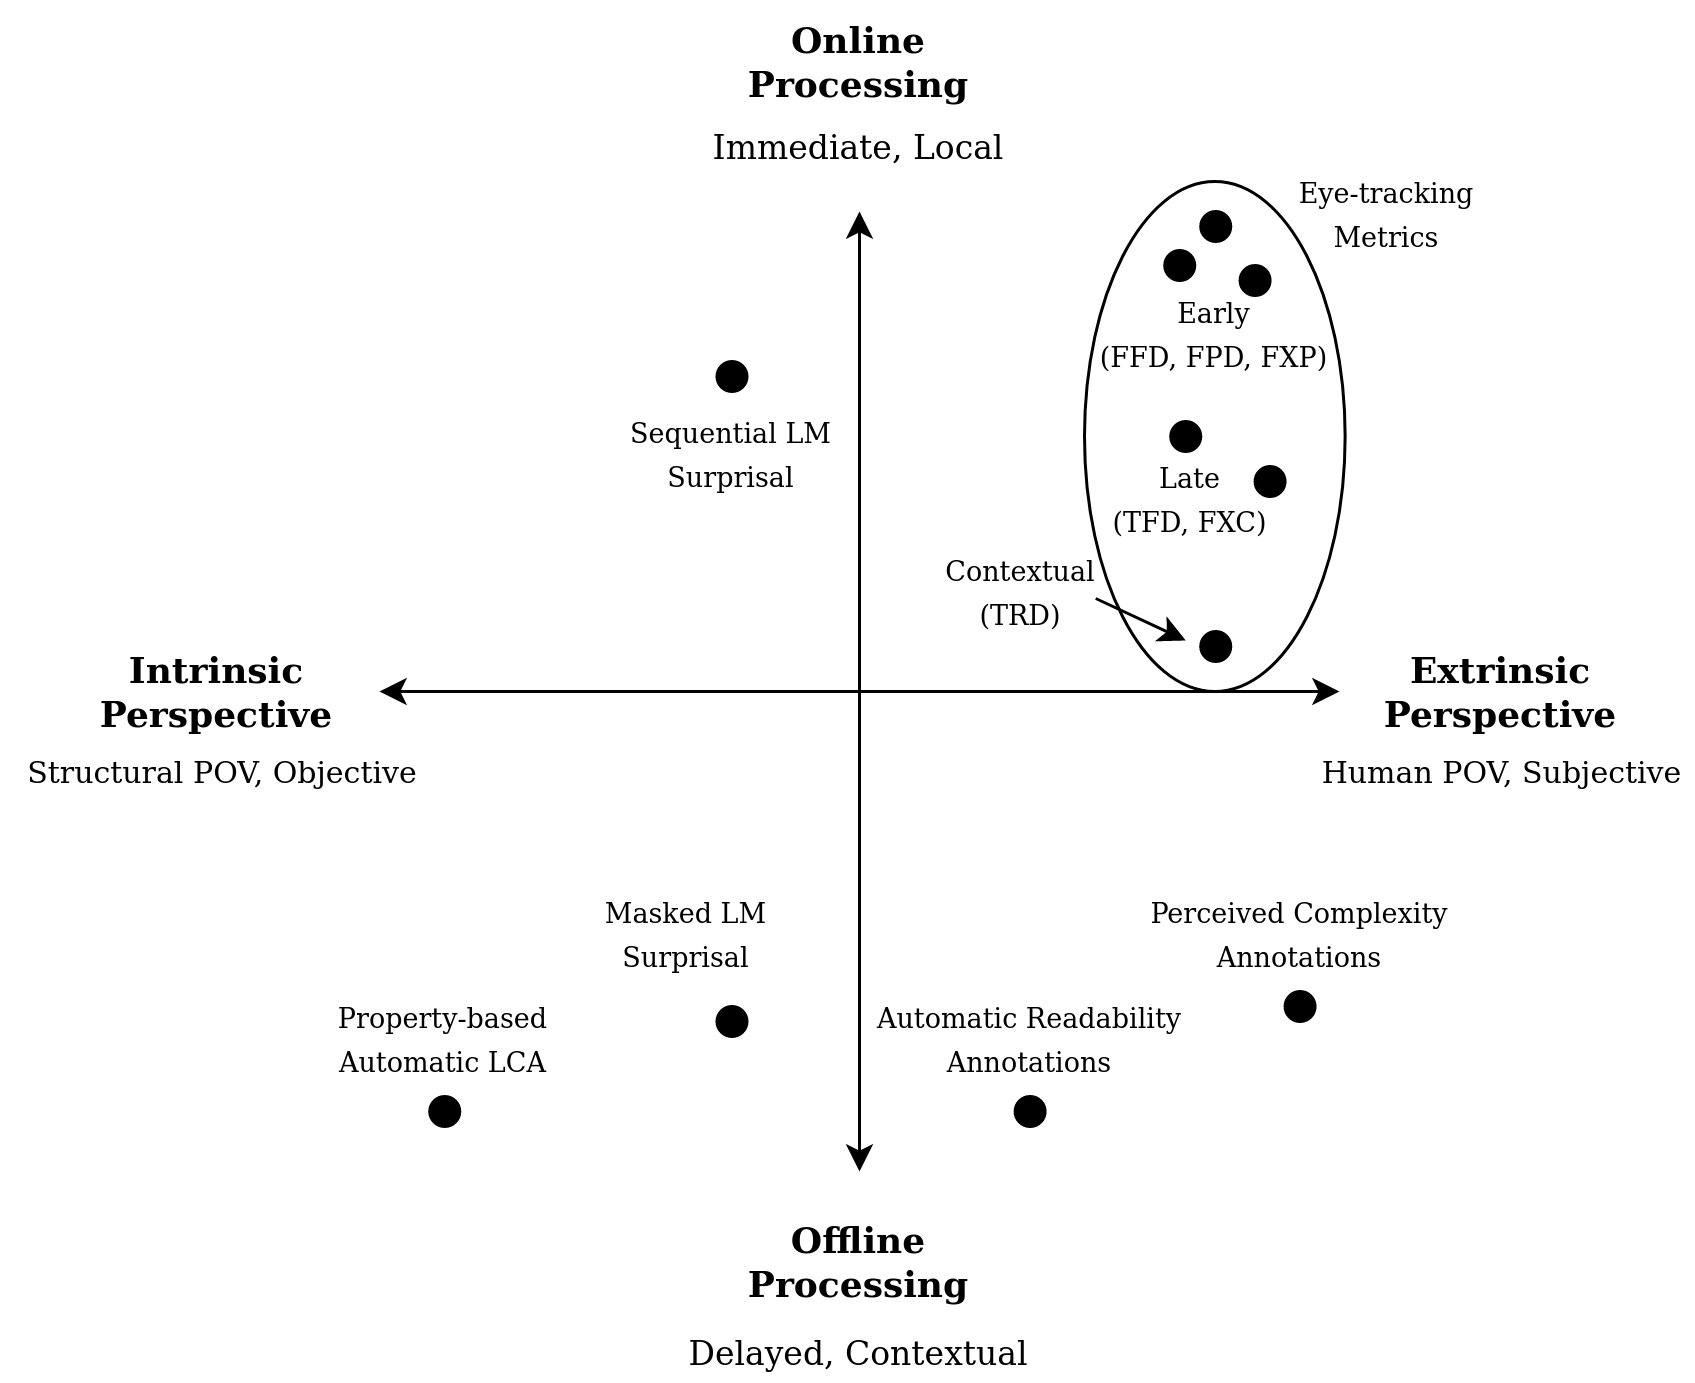
\includegraphics[width=1\linewidth]{figures/1_complexity_compass} \caption{Complexity measures' compass.}\label{fig:compass}
\end{figure}

An additional dimension for categorizing linguistic complexity metrics can be introduced by considering the time at which measures are obtained, relative to the incremental processing paradigm that characterizes natural reading in human subjects. In this context, \emph{processing} is defined as any act aimed at extracting information from linguistic forms and structures, either by employing reasoning (in humans) or through computation (in automatic systems). Again, we can identify the two ends of a spectrum concerning processing modalities, related to the concepts of \textbf{local} and \textbf{global complexity} found in linguistic literature \autocites{edmonds-1999-syntactic}{miestamo-2004-feasibility}{miestamo-2008-grammatical}:

\paragraph{Online processing} Online complexity judgments are collected while a language user, be it a human subject or a computational system, is sequentially processing a text. Online processing is widely explored in the cognitive science literature, where behavioral metrics such are fMRI data and gaze recordings are collected from subjects exposed to locally and temporally-immediate inputs and tasks that require fast processing \autocite{iverson-thelen-1999-hand}. The act of reading is predominantly performed by online cognition \autocite{meyer-rice-1992-prose}, making online measures especially suitable for complexity evaluation for natural reading.

\vspace{-12pt}

\paragraph{Offline processing} Offline complexity judgments are collected at a later time when the language user has a complete and contextual view of the text in its entirety. Again, offline complexity is related to the offline cognition paradigm \autocite{day-2004-religion} typically used in re-evaluations and future planning. In practice, offline evaluation accounts for contextual and cultural factors closely related to individual subjectivity and is poorly captured by immediate online metrics.

\vspace{10pt}

Figure \ref{fig:compass} situates various linguistic complexity metrics in terms of processing modalities and analyzed perspective by including the processing spectrum on the vertical axis. In the next sections, all these measures will be introduced and their use will be motivated in light of this categorization.

\hypertarget{subchap:intrinsic}{%
\section{Intrinsic Perspective}\label{subchap:intrinsic}}

Complexity studies where the intrinsic point of view is adopted rely on annotations describing linguistic phenomena and structures in sentences and aim to map those to complexity levels or ratings, often resorting to formulas parametrized through empirical observation. Given the scarcity of experienced human annotators and the cost of a manual annotation process, computational systems have been primarily employed to extract linguistic information from raw text in an automated yet precise way.

Another intrinsic viewpoint is based on the intuition that frequent constructs should be deemed as less complex than infrequent ones. In this case, terms' co-occurrences are extracted from large corpora, and complexity judgments are derived from their probabilistic likelihood of appearance in a given context. Given the infeasibility of tracking co-occurrences for long sequences in large, typologically-varied corpora, \textbf{computational language models} are usually employed to learn approximations of co-occurrence likelihoods for specific constructs.

While this thesis work only partially addresses the use of these approaches, they will be briefly introduced to provide additional context for understanding extrinsic perspectives and their experimental evaluation.

\hypertarget{subsubchap:structural}{%
\subsection{Structural Linguistic Complexity}\label{subsubchap:structural}}

Language systems can be seen as hierarchies of rules and processes governing various aspects of utterances production and use. For each of those levels, it is possible to identify characteristics leading to higher complexity from a structural standpoint \autocite{sinnemaki-2011-language}:

\begin{itemize}
\item
  A greater number of parts in a specific language level leads to a greater \textbf{syntagmatic complexity} (also known as \emph{constitutional complexity}). This mode is related to the \emph{lexical} and ``superficial'' properties of language, such as the length of words and sentences.
\item
  A greater variety of parts in a specific language level leads to a greater \textbf{paradigmatic complexity} (also known as \emph{taxonomic complexity}). This mode characterizes, in particular, the \emph{phonological} level, where the presence of an elaborated tonal system makes a language more complex \autocite{mcwhorter-2001-world}, the \emph{morphologic} level, where inflectional morphology is usually associated to a higher degree of complexity \autocites{mcwhorter-2001-world}{kusters-2003-linguistic} when compared to the regularity of derivational rules, and the \emph{semantic} level, where polysemic words are generally considered more complex than monosemic ones \autocite{voghera-2001-riflessioni}.
\item
  A greater variety of interrelation modalities and hierarchical structures leads to greater \textbf{organizational and hierarchical complexities}. Those complexity modes are mainly related to the \emph{syntactic level}, where recursive and nested constructs are deemed more complex and possibly determinant in distinguishing human language from animal communication \autocite{hauser-2002-faculty}.
\end{itemize}

Focusing on the syntactic level, we can find multiple factors accounting for greater complexity \autocite{berruto-2011-linguistica}:

\begin{itemize}
\item
  Subordinate clauses preceding the main clause, as in \emph{\underline{If you need help}, let me know"} as opposed to \emph{``Let me know \underline{if you need help}''}.
\item
  Presence of long-range syntactic dependencies between non-contiguous elements, as in \emph{``\underline{The dog} that the cat chased for days \underline{ran away}''} where the subject referent (\emph{dog}) and its verb (\emph{ran}) are far apart in the sentence.
\item
  A high degree of nesting between elements and substructures, as in \emph{``The mouse \textbf{that the cat} \underline{that the dog bit} \textbf{ate} was bought at the fair''} where two nested subordinate clauses introduced by the preposition \emph{that} are present.
\item
  Repeated applications of recursive principles to build utterances with different meanings through the compositionality principle, as in \emph{``I am a huge fan \underline{of fans} of fans of \ldots{} of recursion''}, where the number of recursions defines the final meaning of the sentence.
\end{itemize}

While all those properties are relevant when evaluating an utterance's complexity, only some can be easily extracted from corpora using automatic approaches. In the specific context of this work, the analysis of complexity-related features in Chapter \ref{chap:ex1} makes use of the Profiling--UD tool\footnote{Available at \url{http://linguistic-profiling.italianlp.it}} \autocite{brunato-etal-2020-profiling}, implementing a two-stage process: first, the linguistic annotation process is automatically performed by UDPipe \autocite{straka-etal-2016-udpipe}, a multilingual pipeline leveraging neural parsers and taggers included in the Universal Dependencies initiative \autocite{nivre-etal-2016-universal}. During this step, sentences are tokenized, lemmatized, POS-tagged (i.e., words are assigned lexical categories such as ``Noun'' and ``Verb'') and parsed (i.e., the hierarchical structure of syntactic dependencies is inferred). Then, a set of about 130 linguistic features representing underlying linguistic properties of sentences is extracted from various levels of annotation. Those features account for multiple morphological, syntactic, and ``superficial'' properties related to linguistic complexity. A relevant subset of those features is presented in detail in Appendix \ref{app:ling-feats}.

After deriving linguistic properties from sentences, either automatically as in this study or by manual annotations, two approaches are viable to determine their complexity while maintaining an intrinsic perspective (no human processing data involved):

\vspace{-12pt}

\paragraph{Formula-based Approach} This approach treats linguistic properties of input texts as components of a formula used to determine levels or readability grades. Traditional readability formulas consider multiple factors, such as word length, sentence length, and word frequency. Parameters in those formulas are carefully hand-tuned to match human intuition and correlate well with human-graded readability levels.\footnote{This motivates the previous claim about the interdependence of intrinsic and extrinsic approaches. See Section 2.1 of \textcite{martinc-2019-supervised} for an overview of the most popular metrics for English.}

\vspace{-12pt}

\paragraph{Learning-based Approach} This approach casts the complexity prediction problem in the supervised machine learning framework. More specifically, linguistic parsers are used to predict linguistic properties, and their accuracy on a set of gold-labeled instances is taken as an indicator of complexity. In the case of dependency parsers (i.e., models trained to extract the syntactic structure of a sentence), two evaluation metrics can be used: the \emph{Unlabeled and Labeled Attachment Scores} (UAS and LAS), where the UAS is the percentage of words assigned to the right dependency head and LAS also consider if the dependency relation was labeled correctly.

Both approaches are represented in Figure \ref{fig:compass} under the label ``Property-based Automatic LCA'' and are considered offline since the text is generally not processed incrementally but instead taken as a whole.

\hypertarget{subsubchap:lm-surprisal}{%
\subsection{Language Modeling Surprisal}\label{subsubchap:lm-surprisal}}

The information-theoretic concept of \textbf{surprisal}, also known as \emph{information content} of an event, can be seen as a quantification of the level of surprise caused by a specific outcome: an event that is certain yields no information, while the less probable an event is, the more surprising it gets. Formally, an event \(x\) with probability \(p(x)\) has a surprisal value equal to:

\begin{equation}
I(x) = - \log[p(x)]
\end{equation}

The idea that probabilistic expectations in the context of language reading are related to greater complexity in terms of cognitive processing was formalized by \emph{surprisal theory} \autocites{hale-2001-probabilistic}{hale-2016-information}. Surprisal theory defines processing difficulties \(D\) (which can be considered as proxies of complexity) as directly proportional to the surprisal produced in readers by a word \(w\) given its previous context \(c\) (i.e., preceding words in the sentence):

\begin{equation}
D(w_i|c) \propto -\log p(w_i|c) = -\log p(w_i|w_i-1, w_i-2,\dots, w_0)
\end{equation}

While processing difficulties imply human subjects' presence, \textbf{language models} (LM) can be used to estimate the conceptually similar information-theoretic surprisal without the need of human annotations by learning word occurrences and co-occurrences probabilities from large quantities of text. Concretely, a language model is a probabilistic classifier that learns to predict a probability distribution over words of a vocabulary \(V\) given a large number of contexts \(c\) in which those words occur \autocite{goodman-2001-bit}:

\begin{equation}
p(w_i|c) \quad \forall\ w_i\in V
\end{equation}

After the training procedure it is possible to estimate the probability \(p(s)\) of a sentence \(s\) having length \(m\) as the product of the conditional probabilities assigned to individual words by the language model, given its context:

\begin{equation}
p(s) = p(w_1, \dots, w_m) = \prod_{i=1}^m p(w_i \ |c)
\label{eq:sent-surprisal}
\end{equation}

We can consider the surprisal \(I(s) = -\log p(s)\) as an \emph{intrinsic measure} of linguistic complexity since it is a function of the co-occurrence relations derived by the training corpora. Thus, it describes how likely a construct can be observed in a structurally-sound manner, without relying on human processing data. However, automatic surprisal estimation using language models cannot be considered purely intrinsic since it is highly dependent on a multitude of factors that are arguably ``less objective'' than the linguistic categories of the previous section, such as the type and dimension of the considered context and the corpora employed by the LM to learn words' distributional behavior.

We can categorize modern language models in two broad categories: \textbf{sequential} models (also known as \emph{autoregressive} or \emph{causal} LMs) consider as context only preceding words, while \textbf{bidirectional} models (also known as \emph{masked} LMs) consider both preceding and following words when estimating occurrence probabilities, much like the well-established \emph{cloze test} \autocite{taylor-1953-cloze} in psycholinguistics. Equations \eqref{eq:sent-surprisal-cases} show how the sentence surprisal equation \eqref{eq:sent-surprisal} is adapted in both cases, using the product rule for logarithms:

\begin{equation}
\begin{split}
I_{\mathrm{sequential}}(s) & = - \sum_{i=1}^m \log p(w_i \ | w_1, w_2, \dots, w_{i-1})\\
I_{\mathrm{bidirectional}}(s) & = - \sum_{i=1}^m \log p(w_i \ | w_1, \dots, w_{i-1}, w_{i+1}, \dots, w_m)
\end{split}
\label{eq:sent-surprisal-cases}
\end{equation}

If the LM used to estimate surprisal was sequential, then surprisal estimation could be considered part of the \emph{online processing paradigm} despite the absence of a human subject.\footnote{This is an admittedly simplistic reduction, given the importance of parafoveal processing in reading \autocites{schotter-2012-parafoveal}{schotter-2018-reading}} In the bidirectional case, the estimation of surprisals from the whole context can be assimilated with offline processing practices.

The relation between co-occurrence frequencies estimated by a language model and perception of complexity is one of the aspects that make language models especially suitable for predicting extrinsic complexity metrics, as it will be discussed in Chapter \ref{chap:models}.

\hypertarget{subchap:extrinsic}{%
\section{Extrinsic Perspective}\label{subchap:extrinsic}}

Extrinsic complexity measures elicited from human-produced signals and annotations are the main focus of this thesis work. In this section, three different viewpoints on linguistic complexity assessment from a human perspective are introduced:

\begin{itemize}
\item
  The \textbf{readability} point-of-view, as intended in the context of the \emph{automatic readability assessment} (ARA) task, is concerned with collocating similar textual inputs into difficulty levels that are often predetermined by writers and given a clear semantic interpretation (e.g., easy, medium, hard).
\item
  The \textbf{perceptual} point-of-view, represented by the \emph{perceived complexity prediction} (PCP) task, is based on human annotations of complexity on a numeric scale, taking into account disparate textual inputs presented sequentially to obtain more generalizable complexity annotations. Unlike ARA, PCP annotations are produced by readers after sentence comprehension.
\item
  The \textbf{cognitive} point-of-view, employing cognitive signals collected by specialized machinery (e.g., electrodes, MRI scanners, eye-trackers) as proxies for the linguistic complexity experienced by users. In this work, the focus will be on the \emph{gaze metrics prediction} task, using gaze data collected from subjects during natural reading.
\end{itemize}

All three complexity-related tasks will be introduced alongside recent results in the literature. The corpora on which each task relies upon will also be presented in their respective sections.

\hypertarget{subsubchap:readability}{%
\subsection{Automatic Readability Assessment}\label{subsubchap:readability}}

While the term \emph{readability assessment} is often broadly employed to denote the task of predicting the general reading difficulty of a text, here it is used to describe the typical approach in ARA, relying on corpora categorized by the writer's perception of what is difficult for readers.

We can take as an example the OneStopEnglish (OSE) corpus \autocite{vajjala-lucic-2018-onestopenglish}, which will be used later to study the ARA relation with other complexity tasks in Chapter \ref{chap:ex2}. OSE contains 567 weekly articles from The Guardian newspaper rewritten by language teachers to suit three adult English learners' levels. Each text can be divided into passages spanning one or multiple sentences, each labeled with a readability level (``Elementary'', ``Intermediate'' or ``Advanced'') based on the original writers' judgment. An example of the same passage at different reading levels is provided in Table \ref{tab:ose-example}.

\begin{table}

\caption{\label{tab:ose-example}An OSE Corpus passage at different reading levels.}
\centering
\begin{tabular}[t]{l>{\raggedright\arraybackslash}p{29em}}
\toprule
\textbf{Reading Level} & \textbf{Example}\\
\midrule
Advanced (Adv) & Amsterdam still looks liberal to tourists, who were recently assured by the Labour Mayor that the city’s marijuana-selling coffee shops would stay open despite a new national law tackling drug tourism. But the Dutch capital may lose its reputation for tolerance over plans to dispatch nuisance neighbours
to scum villages made from shipping containers.\\
\addlinespace\hline\addlinespace
Intermediate (Int) & To tourists, Amsterdam still seems very liberal. Recently the city’s Mayor assured them that the city’s marijuana-selling coffee shops would stay open despite a new national law to prevent drug tourism. But the Dutch capitals plans to send nuisance neighbours to scum villages made from shipping containers may damage its reputation for tolerance.\\
\addlinespace\hline\addlinespace
Elementary (Ele) & To tourists, Amsterdam still seems very liberal. Recently the city’s Mayor told them that the coffee shops that sell marijuana would stay open, although there is a new national law to stop drug tourism. But the Dutch capital has a plan to send antisocial neighbours to scum villages made from shipping containers, and so maybe now people wont think it is a liberal city any more.\\
\bottomrule
\end{tabular}
\end{table}

From Table \ref{tab:ose-example} example, it is evident that the reading level of a specific text should be interpreted only in relation to its other versions, i.e., elementary passages are not necessarily straightforward in absolute terms, but rather \emph{less complicated than their intermediate and advanced counterparts}. This affirmation holds for the OSE corpus and other widely-used readability corpora such as the Newsela corpus \autocite{xu-etal-2015-problems}, which contains newspaper articles rewritten by experts to match eleven school grade reading levels. For this reason, and because of its writer-centric perspective relying only on readability judgments formulated by the same writers who composed the passages, readability assessment is fundamentally different from the other extrinsic approaches.\footnote{See \textcite{collins-2014-computational} for a thorough review of ARA approaches.} ARA can be framed as a machine learning task in which a computational model \(m\) is trained to predict the readability level \(y \in \mathcal{Y}\) over a set of labeled examples \(\mathcal{S} = (s_1, s_2, \dots, s_n)\) in two possible ways:

\begin{itemize}
\item
  A simple multiclass classification setting, where the model predicts the level of a single sentence \(s\). In this case, the model outputs a prediction \(m(s) = \hat y \in \mathcal{Y}\). We can then minimize the categorical cross-entropy \(H(y, \hat y)\) between gold and predicted labels during the training process and evaluate the model's performances with standard classification metrics such as precision and recall. This approach is similar to the ones used for other extrinsic metrics but does not account for readability levels' relative nature.
\item
  A multiple-choice scenario, where the model is provided with two semantically equivalent sentences \(s_1, s_2\) at different readability levels (\(s_1 \equiv s_2, y_1 \neq y_2\)) and needs to predict which of the sentences has the highest readability level. In this case, which is more coherent with the relative nature of readability judgments, the model is trained to minimize the binary cross-entropy between gold and predicted labels \(y, \hat y \in \mathcal{Y}_{bin} = \{0,1\}\) corresponding to the position of the more complex sentence in the pair.
\end{itemize}

Expert annotations' effectiveness in determining readers' comprehension was recently questioned, as automatic readability scoring did not show a significant correlation to comprehension scores of participants, at least for the OSE Corpus \autocite{vajjala-lucic-2019-understanding}. However, measuring if this observation holds for other corpora and extrinsic approaches is beyond this thesis's scope.

\hypertarget{subsubchap:pc}{%
\subsection{Perceived Complexity Prediction}\label{subsubchap:pc}}

While ARA measures linguistic complexity in a context-relative and writer-centric sense, the \emph{perceived complexity prediction} (PCP) approach focuses on eliciting absolute complexity judgments directly from target readers, aiming at evaluating difficulties in comprehension rather than production. This approach was pioneered by \textcite{brunato-etal-2018-sentence}, who collected crowdsourced complexity ratings from native speakers for Italian and English sentences and evaluated how different structural linguistic properties contribute to human complexity perception. The use of annotators recruited on a crowdsourcing platform was intended to better grasp the layman's perspective on linguistic complexity, as opposed to ARA expert writers. If collected properly, crowdsourced annotations were shown to be highly reliable for linguistics and computational linguistics research by the survey of \textcite{munro-etal-2010-crowdsourcing}.

\textcite{brunato-etal-2018-sentence} extracted 1200 sentences from both the newspaper sections of the Italian Universal Dependency Treebank (IUDT) \autocite{simi-etal-2014-less} and the Penn Treebank \autocite{mcdonald-etal-2013-universal}, such that those are equally distributed in term of length. To collect human complexity judgments, twenty native speakers were recruited for each language on a crowdsourcing platform. Annotators had to rate each sentence's difficulty on a Likert 7-point scale, with 1 meaning ``very simple'' and 7 ``very complex''. Sentences were randomly shuffled and presented in groups of five per web page, with annotators being given a minimum of ten seconds to complete each page to prevent skimming. The quality of annotations was measured using the Krippendorff alpha reliability, obtaining 26\% and 24\% for Italian and English. Table \ref{tab:pc-example} presents an example of English sentences labeled with multiple annotators' perceived complexity judgments.

\begin{table}

\caption{\label{tab:pc-example}Sample of sentences taken from the English portion of the Perceived Complexity (PC) Corpus with complexity scores from crowdsourced annotators.}
\centering
\begin{tabular}[t]{>{\raggedright\arraybackslash}p{25em}ccccc}
\toprule
\textbf{Sentence} & \textbf{A1} & \textbf{A2} & \textbf{A3} & \textbf{...} & \textbf{A20}\\
\midrule
In other European markets, share prices closed sharply higher in Frankfurt and Zurich and posted moderate rises in Stockholm, Amsterdam and Milan. & 4 & 6 & 7 & ... & 1\\
\addlinespace\hline\addlinespace
The pound strengthened to \$ 1.5795 from \$ 1.5765. & 2 & 1 & 2 & ... & 1\\
\addlinespace\hline\addlinespace
In Connecticut, however, most state judges are appointed by the governor and approved by the state legislature. & 1 & 3 & 3 & ... & 5\\
\addlinespace\hline\addlinespace
When the market stabilized, he added, the firm sold the bonds and quickly paid the loans back. & 2 & 3 & 3 & ... & 3\\
\addlinespace\hline\addlinespace
Paribas already holds about 18.7 \% of Navigation Mixte, and the acquisition of the additional 48 \% would cost it about 11 billion francs under its current bid. & 5 & 2 & 3 & ... & 6\\
\bottomrule
\end{tabular}
\end{table}

As can be expected, PC judgments show significant variability across participants since they cannot be easily framed in a relative setting. Since this work's focus is related to a general notion of complexity, PC judgments are averaged and filtered to obtain a score reflecting the mean perception of complexity of all participants in experimental chapters. The averaged score is later treated as the gold label in a regression task, with machine learning models trained to minimize the \emph{mean square error} between their predictions and gold average annotations. Another possibility, which is not explored in this thesis work, would be to consider only single participants' judgments to model their linguistic complexity perception.

\hypertarget{subsubchap:eye-tracking}{%
\subsection{Gaze Metrics Prediction}\label{subsubchap:eye-tracking}}

Gaze data collected from human subjects during reading can provide us with useful insights from an online extrinsic complexity perspective. Patterns found in both \emph{saccades}, i.e., eye movements from one location to another, and \emph{fixations}, where eyes are relatively stable while fixating a specific region, were shown to be reliably linked to a multitude of linguistic factors \autocite{demberg-keller-2008-data}. Because of this, a linking assumption between overt attention and mental processing can be reasonably established, and gaze metrics can be considered as proxies of cognitive effort, and thus of complexity, at various processing levels.\footnote{See \textcite{rayner-1998-eye} for a comprehensive survey on findings related to eye-tracking research.}

Gaze metrics are widely employed in cognitive processing research because of their multiple benefits: optical eye-tracking systems are non-invasive and relatively inexpensive compared to other approaches that directly measure brain activity, such as electroencephalography (EEG) and all magnetic resonance imaging (MRI) variants. Moreover, gaze data generally have high spatial and temporal precision, limited only by sampling rates, which are generally in the order of few milliseconds. This aspect is crucial for reading research since it allows us to directly associate gaze measures to specific \emph{areas of interest} (AOI, also called region), i.e., small portions of the visual input provided to participants.

\vspace{-12pt}

\paragraph{Gaze data for NLP} Eye-tracking data and other cognitive signals were effectively used in many NLP applications such as POS tagging \autocite{barrett-etal-2016-weakly}, sentiment analysis \autocite{mishra-etal-2017-learning}, native language identification \autocite{berzak-etal-2018-assessing}, and dependency parsing \autocite{strzyz-etal-2019-towards} \emph{inter alia}, often providing modest yet consistent improvements across models and tasks through the combination of gaze features and linguistic features or distributed representations.\footnote{See \textcite{hollenstein-etal-2020-towards} for an exhaustive overview of current approaches and best practices.} In the context of linguistic complexity assessment, eye-tracking data were applied to the ARA task for both monolingual and bilingual participants, obtaining meaningful results for sentence-level classification in easy and hard-to-read categories \autocites{vasishth-etal-2013-what}{ambati-etal-2016-assessing}. For example, \textcite{singh-etal-2016-quantifying} first use a set of linguistic features to learn a reading times model from a set of gaze-annotated sentences and then use models' predicted times over a second set of sentences to perform multiple-choice ARA. \textcite{gonzalez-garduno-sogaard-2018-learning} extend this approach in a multitask learning setting \autocites{caruana-1997-multitask}{ruder-2017-overview}, using eye-movement prediction tasks to produce models able to predict readability levels both from a native speaker and foreign language learner perspective.

\vspace{-12pt}

\paragraph{Collecting Eye-tracking Data} A typical procedure to collect gaze data for reading research, as described by \textcite{schotter-2020-eyetracking}, usually includes the following steps:

\begin{itemize}
\item
  Textual inputs are selected and split by experiment designers, first in areas of interest directly mapped to pixels (for natural reading, usually word boundaries), then over multiple rows, and finally in screens presented to participants. This step should take into account calibration errors to determine the correct level of tolerance for off-word fixations.
\item
  A participant is placed in a room with a display computer used to present visual inputs and a host computer used to record data from the eye-tracker setup. Optical eye-trackers use infrared light beams, which are reflected differently by different parts of the eye, to measure pupil and corneal reflection and track gaze movements at each timestep. The setup is calibrated and validated for each participant to ensure the quality of results.
\item
  Each participant follows the on-screen instructions to complete a reading task trial while remaining at a fixed distance from the screen. A \emph{fixation report} containing events (saccades, fixations, blinks) is produced for each individual on the host computer.
\item
  Finally, a data preprocessing step is taken for each trial to identify and remove artifacts and possibly decide to reject the trial. Some examples of standard practices are the merge of fixations below 80ms due to eye jittering, the exclusion of fixations caused by track loss after blinks, and vertical drift correction \autocite{carr-etal-2020-algorithms}. An \emph{AOI report} containing gaze metrics grouped at AOI level can be produced.
\end{itemize}

\paragraph{Eye-tracking Metrics} Metrics derived from the AOI report contain information about the processing phases in which subjects incur during sentence comprehension. \emph{Early gaze measures} capture information about lexical access and early processing of syntactic structures, while \emph{late measures} are more likely to reflect comprehension and both syntactic and semantic disambiguation \autocite{demberg-keller-2008-data}. The third kind of measures, referred to as \emph{contextual} following the categorization in \textcite{hollenstein-zhang-2019-entity}, capture information from surrounding content. Table \ref{tab:et-metrics} presents a subset of metrics, spanning the three categories, that will be used in the experimental section.\footnote{Appendix \ref{app:et-metrics} contains information about deriving metric values for all corpora.} These metrics represent a minimal group spanning various stages of the reading process and are leveraged to study differences between online and offline processing among extrinsic metrics. In the experimental part, gaze scores are often averaged across participants to reduce noise in measurements and obtain a single label for each metric that can later be used as a reference in a regression setting. The average fixation probability across participants for each AOI is a value comprised in the range \([0,1]\) and represents the proportion of subjects that accessed the region during their first gaze pass.

\begin{table}

\caption{\label{tab:et-metrics}Eye-tracking metrics used in this study.}
\centering
\begin{tabular}[t]{ll>{\raggedright\arraybackslash}p{17em}}
\toprule
\textbf{Type} & \textbf{Metric Name} & \textbf{Description}\\
\midrule
 & First Fixation Duration (FFD) & Duration of the first fixation over the region, including single fixations.\\
\cmidrule{2-3}
 & First Pass Duration (FPD) & Duration of the first pass over a region.\\
\cmidrule{2-3}
\multirow[t]{-3}{*}{\raggedright\arraybackslash Early} & Fixation Probability (FXP) & Boolean value reflecting if the region was fixated or skipped during the first pass.\\
\cmidrule{1-3}
 & Fixation Count (FXC) & Number of total fixations over a region.\\
\cmidrule{2-3}
\multirow[t]{-2}{*}{\raggedright\arraybackslash Late} & Total Fixation Duration (TFD) & Sum of all fixation durations over a region.\\
\cmidrule{1-3}
Contextual & Total Regression Duration (TRD) & Duration of regressive saccades performed after a region's first access and before going past it.\\
\bottomrule
\end{tabular}
\end{table}

\paragraph{Eye-tracking Corpora} The experimental part of this thesis work leverages four widely used eye-tracking resources: the Dundee corpus \autocite{kennedy-etal-2003-dundee}, the GECO corpus \autocite{cop-etal-2017-presenting}, the ZuCo corpus \autocite{hollenstein-2018-zuco}, and ZuCo 2.0 \autocite{hollenstein-etal-2020-zuco}. There are multiple reasons behind the choice of using multiple gaze-annotated corpora for this study. First, those corpora span different domains and provide us with a better intuition of what structures are perceived as complex in different settings and by different pools of subjects. Secondly, neural-network-based complexity models used in this work greatly benefit from a broader availability of annotated data to achieve higher performances in predicting eye-tracking metrics. Finally, while all corpora relied on different procedures and instrumentation, they are all derived from very similar experimental settings (i.e., natural reading on multiple lines), and can be easily merged after an individual normalization procedure \autocite{hollenstein-zhang-2019-entity}. Table \ref{tab:et-corpora} presents some descriptive statistics of the four corpora.

\begin{itemize}
\item
  The \textbf{Dundee Corpus} developed by \textcite{kennedy-etal-2003-dundee} contains gaze data for ten native English speakers tasked with reading twenty newspaper articles from \emph{The Independent}. The English section of the Dundee corpus includes 51,240 tokens in 2368 sentences. Texts were presented to subjects on a screen five lines at a time and recorded using a \emph{Dr.~Bois Oculometer Eyetracker} with 1 kHz monocular (right) sampling. Dundee corpus data are the oldest among selected corpora and have been extensively used in psycholinguistic research about naturalistic reading.
\item
  The \textbf{Ghent Eye-tracking Corpus} (GECO) by \textcite{cop-etal-2017-presenting} was created more recently to study eye movements of both monolingual and bilingual subjects during naturalistic reading of the novel \emph{The Mysterious Affair at Styles} by Agatha \textcite{christie-2003-mysterious}. In the context of this work, only the monolingual portion collected from 14 native English speakers is used, comprising 56,409 tokens in 5,387 sentences. Eye movements were recorded with an \emph{EyeLink 1000} system with 1 kHz binocular sampling (only right eye movements were considered), and the text was presented one paragraph at a time.
\item
  The \textbf{Zurich Cognitive Language Processing Corpus} (ZuCo) by \textcite{hollenstein-2018-zuco} is a dataset including both eye-tracking and EEG measurements collected simultaneously during both natural and task-oriented reading. The corpus contains 1100 English sentences from the Stanford Sentiment Treebank \autocite{socher-etal-2013-recursive} and the Wikipedia dump used in \textcite{culotta-etal-2006-integrating} with gaze data for 12 adult native speakers. Only the first two portions are used for the present work since they contain natural reading data, totalizing 700 sentences and 13,630 tokens. The text was presented on-screen one sentence at a time, and data were collected with an \emph{EyeLink 1000} as for GECO.
\item
  \textbf{ZuCo 2.0} is an extension of ZuCo, including 739 sentences extracted from the Wikipedia corpus by \textcite{culotta-etal-2006-integrating}. Only the 349 sentences for which natural reading data were collected are used, and the 100 duplicates shared with ZuCo to evaluate differences in setup and participants are removed. Data were collected from 18 native English speakers using an \emph{EyeLink 1000 Plus} with 500 kHz sampling.
\end{itemize}

\begin{table}

\caption{\label{tab:et-corpora}Descriptive statistics of eye-tracking corpora.}
\centering
\begin{tabular}[t]{lcc>{\centering\arraybackslash}p{8em}>{}c|c}
\toprule
\textbf{} & \textbf{Dundee} & \textbf{GECO} & \textbf{ZuCo} & \textbf{ZuCo 2.0} & \textbf{Total}\\
\midrule
domain(s) & news & literature & movie reviews, Wiki articles & Wiki articles & -\\
\# of sentences & 2368 & 5387 & 700 & 349 & 8804\\
mean sent. length & 21.64 & 10.47 & 19.47 & 19.51 & 17.77\\
\# of tokens & 51240 & 56409 & 13630 & 6810 & 128089\\
unique token types & 9928 & 6155 & 4650 & 2521 & 16320\\
mean token length & 4.88 & 4.6 & 5.05 & 5.01 & 4.89\\
mean fix. duration & 200 & 210 & 117 & 117 & 161\\
mean gaze duration & 280 & 234 & 139 & 134 & 197\\
\bottomrule
\end{tabular}
\end{table}

Tokens are obtained using whitespace tokenization, which is the same approach used to perform gaze annotations across all eye-tracking corpora. Mean sentence length is expressed in number of tokens, and the number of unique types is computed as the size of the vocabulary after removing punctuation from all tokens. Approximately 128,000 tokens annotated with gaze recordings from multiple participants were used in the experiments of Chapters \ref{chap:ex2} and \ref{chap:ex3}, while only GECO was used for the analysis of Chapter \ref{chap:ex1}. Similarly to the PCP task, scores were averaged across subjects to reduce noise and obtain general estimates: in particular, reading times that were missing due to skipping were considered as having the lowest duration across annotators, which is a practice commonly used in literature. Again, considering individual participants' scores is deemed attractive in a personalization perspective but far beyond this work's scope.

\hypertarget{subchap:garden-path}{%
\section{Garden-path Sentences}\label{subchap:garden-path}}

\begin{figure}
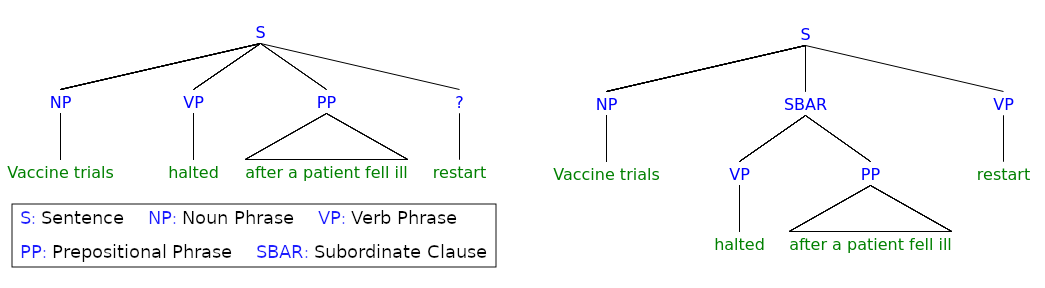
\includegraphics[width=1\linewidth]{figures/1_syntax_trees_gp} \caption{Syntax trees for the initial and complete parse of garden-path example (1).}\label{fig:syntax-trees}
\end{figure}

\textbf{Garden-path sentences}, named from the expression ``leading down the garden path'' implying deception, are grammatically correct sentences that create a momentarily ambiguous interpretation in readers. The initial interpretation is later falsified by words encountered during sequential reading, becoming a significant source of processing difficulties. For this reason, garden-path constructions are used to evaluate models of linguistic complexity in the experiments of Chapter \ref{chap:ex3}. Consider the following recent headline by the newspaper \emph{The Guardian}:\footnote{\url{https://twitter.com/drswissmiss/status/1304856856649756673}}

\begin{quote}
\begin{enumerate}
\def\labelenumi{(\arabic{enumi})}
\tightlist
\item
  Vaccine trials halted after patient fell ill \underline{restart}.
\end{enumerate}
\end{quote}

Readers exposed to (1) tend to initially prefer the interpretation in which halted acts as the main verb of the sentence in simple past, i.e., \emph{``Vaccine trials halted after patient fell ill.''} is interpreted as a well-formed and semantically meaningful sentence. When the verb \emph{restart} is reached, it suddenly becomes evident that the original parse would lead to an ungrammatical sentence, and a reanalysis requiring nontrivial cognitive processing is triggered. In conclusion, one understands that \emph{halted} is used as a passive participle, and \emph{Vaccine trials} are the subordinate clause's direct object, as shown in Figure \ref{fig:syntax-trees}. We can rephrase the sentence with minimal changes to make it unambiguous:

\begin{quote}
\begin{enumerate}
\def\labelenumi{(\arabic{enumi})}
\setcounter{enumi}{1}
\tightlist
\item
  Vaccine trials that were halted after patient fell ill restart.
\end{enumerate}
\end{quote}

The choice for the initial parse can be explained in terms of frequency of occurrence: subject-verb-object sentences are encountered much more frequently than ones containing reduced relatives in everyday settings, making the first parse more likely \autocite{fine-2013-rapid}. We refer to the verb causing the reanalysis as \emph{disambiguator}, and to the difference in cognitive processing between (1) and (2), measured using proxies such as gaze metrics, as \emph{garden-path effect} \autocite{bever-1970-cognitive}.

\textcite{schjindel-linzen-2020-single} present two families of cognitive processing theories trying to motivate the underlying difficulties in which humans incur with garden-path sentences:

\begin{itemize}
\item
  \emph{Two-stage accounts} assume that readers consider only one or a subset of possible parses for each sentence that it is reading \autocites{gibson-1991-computational}{jurafsky-1996-probabilistic}, and processing difficulties arise as a consequence of the reanalysis process need to reconstruct parses that were initially disregarded or not considered \autocite{frazier-1978-sausage}.
\item
  \emph{One-stage accounts} such as \textbf{surprisal theory} \autocites{hale-2001-probabilistic}{levy-2008-expectation} instead consider difficulties produced by garden paths as the products of a single processing mechanism. Dispreferred parses are not discarded, but rather associated with a lower probability compared to that of likely ones: ``processing difficulty on every word in the sentence, including the disambiguating words in garden-path sentences, arises from the extent to which the word shifts the reader's subjective probability distribution over possible parses'' \autocite{schjindel-linzen-2020-single}.
\end{itemize}

There are multiple types of garden-path sentences, usually categorized based on their respective syntactic ambiguities \autocite{frazier-1978-comprehending}. In this work, two classic garden-path families are studied in three different settings using examples taken from \textcite{futrell-etal-2019-neural}. The first type is the \textbf{MV/RR ambiguity} presented in example (1), and repeated in (3a):

\begin{quote}
\begin{enumerate}
\def\labelenumi{(\arabic{enumi})}
\setcounter{enumi}{2}
\item
  \begin{enumerate}
  \def\labelenumii{\alph{enumii}.}
  \tightlist
  \item
    The woman brought the sandwich \underline{fell} in the dining room. \footnotesize\text{{[}RED., AMBIG.{]}}
  \end{enumerate}
\end{enumerate}
\end{quote}

\begin{quote}
\begin{enumerate}
\def\labelenumi{\alph{enumi}.}
\setcounter{enumi}{1}
\tightlist
\item
  The woman who was brought the sandwich fell in the dining room. \footnotesize\text{{[}UNRED., AMBIG.{]}}
\end{enumerate}
\end{quote}

\begin{quote}
\begin{enumerate}
\def\labelenumi{\alph{enumi}.}
\setcounter{enumi}{2}
\tightlist
\item
  The woman given the sandwich fell in the dining room. \footnotesize\text{{[}RED., UNAMBIG.{]}}
\end{enumerate}
\end{quote}

\begin{quote}
\begin{enumerate}
\def\labelenumi{\alph{enumi}.}
\setcounter{enumi}{3}
\tightlist
\item
  The woman who was given the sandwich fell in the dining room. \footnotesize\text{{[}UNRED., UNAMBIG.{]}}
\end{enumerate}
\end{quote}

The label MV/RR indicates that \emph{brought} can be initially parsed either as the main verb (MV) in the past tense of the clause or as a passive participle introducing a reduced relative (RR) clause, which postmodifies the subject. It is possible to rewrite the sentence by changing the ambiguous verb to an equivalent one having different forms for simple past and past participle (such as \emph{gave} vs. \emph{given}). In this case, we expect that the difference in cognitive processing for the disambiguator \emph{fell} between the reduced (3c) and the unreduced (3d) version is smaller since the ambiguity is ruled out from the beginning.

The second type of ambiguity is the \textbf{NP/Z ambiguity} presented in (4a):

\begin{quote}
\begin{enumerate}
\def\labelenumi{(\arabic{enumi})}
\setcounter{enumi}{3}
\item
  \begin{enumerate}
  \def\labelenumii{\alph{enumii}.}
  \tightlist
  \item
    As the criminal shot the woman \underline{yelled} at the top of her lungs. \footnotesize\text{{[}TRANS., NO COMMA{]}}
  \end{enumerate}
\end{enumerate}
\end{quote}

\begin{quote}
\begin{enumerate}
\def\labelenumi{\alph{enumi}.}
\setcounter{enumi}{1}
\tightlist
\item
  As the criminal fled the woman yelled at the top of her lungs. \footnotesize\text{{[}INTRANS., NO COMMA{]}}
\end{enumerate}
\end{quote}

\begin{quote}
\begin{enumerate}
\def\labelenumi{\alph{enumi}.}
\setcounter{enumi}{2}
\tightlist
\item
  As the criminal shot, the woman yelled at the top of her lungs. \footnotesize\text{{[}TRANS., COMMA{]}}
\end{enumerate}
\end{quote}

\begin{quote}
\begin{enumerate}
\def\labelenumi{\alph{enumi}.}
\setcounter{enumi}{3}
\tightlist
\item
  As the criminal fled, the woman yelled at the top of her lungs. \footnotesize\text{{[}INTRANS., COMMA{]}}
\end{enumerate}
\end{quote}

The label NP/Z is used to indicate that the transitive verb \emph{shot} can initially be understood to have either have a noun phrase (NP) object like \emph{the woman} or a zero (Z), i.e., null object if used intransitively as it is the case for (4a). The sentence can be rewritten by substituting the transitive verb generating the ambiguity with an intransitive one, e.g., replacing \emph{shot} with \emph{fled} in (4b), by adding a disambiguating comma to force the null-object parse as in (4c), or by doing both as in (4d). We expect that the cognitive processing difference for the disambiguator \emph{yelled} between the ambiguous (4a) and the unambiguous (4b) is smaller since the ambiguity is ruled out from the beginning.

As an additional NP/Z setting evaluation, consider the case in which an overt object is added to the verb introducing the ambiguity:

\begin{quote}
\begin{enumerate}
\def\labelenumi{(\arabic{enumi})}
\setcounter{enumi}{4}
\item
  \begin{enumerate}
  \def\labelenumii{\alph{enumii}.}
  \tightlist
  \item
    As the criminal shot the woman \underline{yelled} at the top of her lungs. \footnotesize\text{{[}NO OBJ., NO COMMA{]}}
  \end{enumerate}
\end{enumerate}
\end{quote}

\begin{quote}
\begin{enumerate}
\def\labelenumi{\alph{enumi}.}
\setcounter{enumi}{1}
\tightlist
\item
  As the criminal shot his gun the woman yelled at the top of her lungs. \footnotesize\text{{[}OBJ., NO COMMA{]}}
\end{enumerate}
\end{quote}

\begin{quote}
\begin{enumerate}
\def\labelenumi{\alph{enumi}.}
\setcounter{enumi}{2}
\tightlist
\item
  As the criminal shot, the woman yelled at the top of her lungs. \footnotesize\text{{[}NO OBJ., COMMA{]}}
\end{enumerate}
\end{quote}

\begin{quote}
\begin{enumerate}
\def\labelenumi{\alph{enumi}.}
\setcounter{enumi}{3}
\tightlist
\item
  As the criminal shot his gun, the woman yelled at the top of her lungs. \footnotesize\text{{[}OBJ., COMMA{]}}
\end{enumerate}
\end{quote}

Again, we expect that the difference in cognitive processing for \emph{yelled} is higher in the non-object pair (5a)-(5c), where the first item is a garden-path sentence, rather than in the pair (5b)-(5d) where both sentences are unambiguous.

\paragraph{Gaze metrics and Garden-path Sentences} As can be intuitively assumed, garden-path effects are reflected in gaze metrics collected during natural reading. Multiple studies have focused on quantifying the difference between garden-path sentences and their unambiguous counterparts on reading times in human subjects. \textcite{sturt-etal-1999-structural} found a massive delay of 152ms for each word in the disambiguating region of NP/Z sentences. \textcite{grodner-etal-2003-against} estimate an average delay of 64ms over the disambiguating region for NP/Z constructs using 53 college students' reading times over a set of 20 ambiguous sentences. More recently, \textcite{prasad-linzen-2019-much} recorded eye measurements for 224 participants recruited through Amazon Mechanical Turk on the same set of NP/Z sentences as \textcite{grodner-etal-2003-against}, finding a much lower average delay of 28ms, and suggesting an overestimation in previous studies due to small sample size and publication contingency to significant results. \textcite{prasad-linzen-2019-self} collected self-paced reading times from 73 participants recruited on the Prolific Academic crowdsourcing platform and measured an average delay of 22ms over the disambiguating region for MV/RR constructs.

Given the high variability in results across studies, it can be hypothesized that the way in which stimuli were presented to subjects plays a significant role in determining the magnitude of garden-path effects \autocite{schjindel-linzen-2018-modeling}. For example, a sentence presented word-by-word to subjects may yield more ecologically valid reading times estimates than a sentence presented region-by-region. Another problematic factor involves constraining the impact of garden-path effects to the disambiguating region: first, because \emph{parafoveal preview effects may slightly anticipate the start of the effect} \autocites{schotter-2012-parafoveal}{schotter-2018-reading}; and second, because due to \emph{spillover} \autocite{mitchell-1984-evaluation}, a phenomenon in which the surprisal of a word influences the reading times for itself and at least three subsequent words \autocite{smith-levy-2013-effect}, reading times of the disambiguating region are influenced by preceding words, and influence subsequent ones, spreading the garden-path effect on a much broader context. For this reason, eye-tracking metrics are studied for all sentence regions in the experiments of Chapter \ref{chap:ex3}.

\titlespacing{\chapter}{0pt}{0pt}{35pt}

\begin{savequote}
Now it would be very remarkable if any system existing in the real world
could be exactly represented by any simple model. {[}\ldots{}{]} For
such a model there is no need to ask the question ``Is the model
true?''. The only question of interest is ``Is the model illuminating
and useful?''.
\qauthor{--- George \textcite{box-1976-science}, \emph{Science and Statistics}}\end{savequote}



\titlespacing*{\chapter}{0pt}{80px}{35pt}

\hypertarget{chap:models}{%
\chapter{\texorpdfstring{\textbf{Models of Linguistic Complexity}}{Models of Linguistic Complexity}}\label{chap:models}}

\minitoc 

\chaptermark{Models of Linguistic Complexity}

Standard linguistic complexity studies analyze complexity annotations produced by human subjects to evaluate how specific language structures influence our perception of complexity under various viewpoints. For example, one can derive insights about early cognitive processing by looking at early gaze metrics, like first pass duration and first fixation duration, or study language comprehension by evaluating perceived complexity annotations. These approaches rely on a single implicit assumption: that \emph{complexity annotations contain enough information to reflect the input's underlying complexity properties} appropriately. Without this premise, there would be a complete disconnect between human subjective perception, as reflected by annotations and linguistic structures. Given the ever-growing compelling evidence derived from carefully-planned complexity research, I argue that this is a relatively safe assumption to be made.

This work instead adopts a modeling-driven approach for the study of linguistic complexity. Annotations produced by human subjects still play a fundamental role in this context. However, instead of acting as the main subject of analysis, they are used as a source of distant supervision to create computational models of linguistic complexity. More specifically, machine learning models are trained to predict complexity annotation from raw input text by minimizing a task-specific loss function. The \textbf{learning step} here is fundamental, given the connection mentioned above between linguistic complexity and knowledge acquisition. After the training process, human annotations are put aside, and the model itself is studied as a complexity-sensitive subject: in particular, this study focuses on how the information encoded in the parameters of complexity-trained models is related to structural linguistic properties (Chapter \ref{chap:ex1}), how this information differs when models are exposed to different complexity perspectives during training (Chapter \ref{chap:ex2}) and finally how the encoded knowledge affects models' generalization capabilities over unseen constructs (Chapter \ref{chap:ex3}).

While this approach still relies on the \textbf{annotation pertinence assumption} stated above, it requires making a second, stronger hypothesis: that \emph{models employed can grasp a significant portion of the relations subsisting between language structures and complexity perspectives}. This assumption can be further declined in two requirements. First, from a \textbf{conceptual} point-of-view, we must ensure that the model architecture is endowed with meaningful inductive biases concerning what is currently known about linguistic complexity. This includes having sufficient approximation capabilities to capture linguistic complexity phenomena, which are likely to be highly-nonlinear functions of the input. From a \textbf{functional} perspective, then, we should confirm that the quality of model predictions is sufficiently close to human-produced annotations to make their production mechanisms worth investigating.

This chapter justifies the selected modeling approach and introduces models later employed in complexity assessment experiments. Section \ref{subchap:desiderata} discusses the conceptual requirements for linguistic complexity modeling and motivates the choice of pretrained \textbf{neural language models} as primary subjects of this thesis work. Section \ref{subchap:nlm} presents the architectures used in experimental sections and their desirable properties regarding the encoding of linguistic structures in latent representations. Finally, Section \ref{subchap:analyzing-nlm} presents the challenge of interpreting NLM's representations and behaviors and introduces various interpretability approaches used throughout this study.

\hypertarget{subchap:desiderata}{%
\section{Desiderata for Models of Linguistic Complexity}\label{subchap:desiderata}}

From the in-depth analysis of Chapter \ref{chap:ling-comp}, we can distill some general desiderata for an idealized LCA model \(M^*\). From a linguistic perspective:

\begin{itemize}
\item
  \(M^*\) \emph{should distinguish between lexical forms and be informed about their probability of occurrence.} This is a basic (although fundamental) step given the importance of words' variety and frequency in determining our perception of complexity.
\item
  \(M^*\) \emph{should be aware of syntactic structures and sensitive to their properties.} As we saw with garden-path sentences, atypical or ambiguous syntax constructs are among the most prominent factors for determining the magnitude of processing difficulties. An ideal model should map complex syntactic constructs to higher complexity scores and discriminate potentially ambiguous or problematic structures from regular ones, even when changes in the form are minimal (e.g., when a single comma is missing).
\item
  \(M^*\) \emph{should capture semantic information and relations between entities.} Ideally, this means the ability to frame agents, patients, and actions in a semantic context and evaluate how likely or typical the latter is. For example, semantically unrelated entities occurring together in a sentence should produce an increase in processing difficulties. This includes the ability to disambiguate polysemic terms (e.g., ``fly'' verb vs.~noun) given the surrounding context.
\end{itemize}

Then, from a technical standpoint:

\begin{itemize}
\item
  \(M^*\) \emph{should not rely on hand-crafted features to represent language}. This is an implicit requirement since this study aims to analyze how the model autonomously learns to represent language in its parameters while simultaneously encoding information about its complexity. Chapter \ref{chap:ex1} presents how complexity models with hand-crafted features compare to those selected for the study.
\item
  \(M^*\) \emph{should not rely too heavily on labeled data.} Complexity datasets presented in Chapter \ref{chap:ling-comp} are usually composed of a few thousand labeled examples. While this may seem a lot to our eyes, a language model may require a lot more information to achieve sufficient generalization capabilities. A viable option in this context, as we will see with NLMs, is to prime models with general linguistic knowledge through an unsupervised pretraining procedure before training them on complexity-related tasks.
\item
  \(M^*\) \emph{should be sufficiently interpretable.} Ideally, we would like to draw direct causal relations from input properties to complexity prediction in a consistent way across complexity perspectives. More realistically, we need at least to find coherent patterns between the model's inputs and its predictive behaviors.
\end{itemize}

Most standard modeling approaches fail to encompass even a small subset of those non-trivial requirements. For example, one can consider modeling complexity properties with static word representations \autocite{turian-etal-2010-word} such as Word2Vec or GloVe embeddings \autocites{mikolov-etal-2013-efficient}{pennington-etal-2014-glove}. In these approaches, feature vectors representing words are learned by a neural network through a pretraining procedure to model word co-occurrences. While these approaches were shown to capture a significant amount of semantic information while reducing the dependence on labeled data thanks to pretraining, static word embeddings generally yield modest results when employed for syntactic predictions \autocite{andreas-klein-2014-much}. Moreover, since the model learns a direct mapping \(f: t_i \rightarrow \textbf{v}_i\) from lexical forms to vectorial representations, polysemic terms are reduced to single context-independent representation, and contextual information that often plays a crucial role in determining complexity is mixed and diluted.

Among more sophisticated modeling approaches for representing language, I argue that modern \textbf{neural language models} (NLMs) are the approaches that yield a better match for the requirements stated above. These models consist of multi-layer neural networks \autocite{goodfellow-etal-2016-deep} pretrained using standard language modeling or masked language modeling training objectives to produce \textbf{contextualized word embeddings}, which were shown to be very effective in downstream syntactic and semantic tasks \autocite{peters-etal-2018-deep} even with relatively few labeled examples. Moreover, being language models, NLMs predict a probability distribution over their vocabulary at each step, enabling us to compute information-theoretic metrics such as surprisal that we saw being conceptually close to one-stage cognitive processing accounts. Finally, their high parameter counts and the presence of self-attention mechanisms \autocites{bahdanau-etal-2015-neural}{vaswani-etal-2017-attention} as learned weighting functions suggests that NLMs might be capable of learning to approximate highly nonlinear functions effectively.

The most significant downside of NLMs in the context of our analysis is their opaqueness. As for most neural networks, the nonlinear multi-layer structure that characterizes NLMs makes them incredibly valid function approximators. At the same time, though, it hinders our efforts in interpreting their behaviors \autocite{samek-etal-2019-explainable}. Because of this fact, in recent years, we witnessed a surge in approaches trying to ``open the black box'' of neural networks by using various techniques borrowed from information theory \autocite{shwartz-tishby-2017-opening} and cognitive science \autocite{kriegeskorte-etal-2008-representational}. Given the wide availability of these approaches, this work joins the choir of interpretability researchers and argues that studying how such performant models encode their knowledge about language complexity is still a matter of interest and worth exploring. In the next section, the architecture and training process of NLMs will be formalized, and their properties will be described in detail.

\hypertarget{subchap:nlm}{%
\section{Neural Language Models: Unsupervised Multitask Learners}\label{subchap:nlm}}

The objective of natural language processing applications such as \emph{summarization}, \emph{machine translation}, and \emph{dialogue generation} is to produce text that is both \textbf{fluent} and contextually accurate. As we saw in Chapter \ref{chap:ling-comp}, a text's fluency can also be used as a significant factor in determining its complexity from a linguistic viewpoint. A possible approach to establishing a sentence's fluency is to rely on \textbf{relative frequency estimates} for words in large corpora. Consider a sentence \(s\) and a large corpus \(\mathcal{C}\). We can estimate its probability of occurrence in natural language as:

\begin{equation}
P(s) = \frac{\text{count}(s)}{|\mathcal{C}|}
\end{equation}

While this is an unbiased estimator since it converges to the actual frequency value when the corpus size is sufficiently large, it is both very data-reliant and highly unreliable. If a sentence happens to be absent in \(\mathcal{C}\), it will be assigned probability equal to zero. Therefore, we need to rely on other approaches, such as language models, to obtain reliable estimates from limited training datasets.

As we saw in Chapter \ref{subsubchap:lm-surprisal}, language models assign probabilities to sequences of tokens. Formally, this can be framed as learning words' conditional probability distributions given their context, either \emph{preceding} or \emph{bidirectional} depending on the language modeling approach. I will here refer to sequential language models unless otherwise mentioned.

Language models are trained on sequences \(\textbf{x} = \langle x_1, \dots, x_n \rangle\) composed by \(n\) tokens taken from a predefined vocabulary \(\mathcal{V}\). Each token \(x_i\) can be represented as a one-hot encoded vector \(x_i \in \{0,1\}^{|\mathcal{V}|}\), and the probability of sequence \(\textbf{x}\) is factored using the chain rule:

\begin{equation}
P(\textbf{x}) = \prod_{t=1}^{n}\,P(x_t\,|\,x_1,\dots,x_{t-1})
\end{equation}

After the training process, we can use the likelihood that the model assigns to \textbf{held-out data} \(\textbf{y}\) treated as a single stream of \(m\) tokens as an intrinsic evaluation metric for the quality of its predictions:

\begin{equation}
\ell(\textbf{y}) = \sum_{t=1}^m \log P(x_t|x_1,\dots,x_{t-1})
\end{equation}

\(\ell(\textbf{y})\) can be rephrased in terms of \textbf{perplexity}, an information-theoretic metric independent from the size of the held-out set:

\begin{equation}
\text{PPL}(\textbf{y}) = 2^{-\ell(\textbf{y})/m}
\end{equation}

\(\text{PPL}\) is equal to 1 if the language model is perfect (i.e., predicts all tokens in the held-out corpus with probability 1) and matches the vocabulary size \(|\mathcal{V}|\) when the model assign a uniform probability to all tokens in the vocabulary (a ``random'' language model):

\begin{align} 
\log_2(\textbf{y}) = \sum_{t=1}^m \log_2 \frac{1}{|\mathcal{V}|} = - \sum_{t=1}^m \log_2 |\mathcal{V}| = -m \log_2 |\mathcal{V}| \\
\text{PPL}(\textbf{y}) = 2^{\frac{1}{m}m\log_2 |\mathcal{V}|} = 2^{\log_2 |\mathcal{V}|} = |\mathcal{V}|
\end{align}

Perplexity represents the number of bits required to encode the average word in the corpora. For example, reporting a perplexity score of 10 over a held-out corpus means that the language model will predict on average words with the same accuracy as if it had to choose uniformly and independently across ten possibilities for each word.

While tokens used by language models generally correspond to words in most NLP pipelines, recent language modeling work highlighted the effectiveness of using subword tokens \autocites{sennrich-etal-2016-neural}{wu-etal-2016-google}{kudo-richardson-2018-sentencepiece} or even single characters to further improve LM's generalization performances. In particular, models used in this work rely on SentencePiece and Byte-Pair Encoding (BPE) subword tokenization \autocites{sennrich-etal-2016-neural}{kudo-richardson-2018-sentencepiece}. The SentencePiece algorithm derives a fixed-size vocabulary from word co-occurrences in a large corpus and treats whitespace as a normal symbol by converting it to ``\textbf{\_}'', while BPE does the same using the ``Ġ'' character. For example:

\begin{quote}
\textbf{Input sentence:} Heteroscedasticity is hard to model!
\end{quote}

\begin{quote}
\textbf{SentencePiece tokenization:} \textbf{\_}Hetero s ced astic ity \textbf{\_}is \textbf{\_}hard \textbf{\_}to \textbf{\_}model !
\end{quote}

\begin{quote}
\textbf{BPE tokenization:} H eter os ced astic ity Ġis Ġhard Ġto Ġmodel !
\end{quote}

where whitespaces correspond to separators after tokenization. From the example, we can observe that frequent words like \emph{hard}, \emph{to} and \emph{model} are treated similarly by both tokenizers, while rare words like \emph{heteroscedasticity} are split into subwords depending on their observed frequency inside the tokenizer's training corpus.

In recent years n-gram language models, which were the most common approach to estimate probabilities from relative frequencies, have been largely supplanted by neural networks. A significant advantage of neural approaches is the overcoming of context restrictions: relevant information can be incorporated from arbitrarily distant contexts while preserving the tractability of the problem from both a statistical and a computational viewpoint.

Neural language models treat language modeling as a \emph{discriminative} learning task aimed at maximizing the log conditional probability of a corpus. Formally, the probability distribution \(p(x|c)\) is reparametrized as the dot product of two dense numeric vectors \(\boldsymbol\theta_x, \boldsymbol h_c \in \mathbb{R}^H\) under a softmax transformation:

\begin{equation}
P(x|c) = \frac{\exp(\boldsymbol\theta_x \cdot \boldsymbol h_c)}{\sum_{x'\in\mathcal{V}} \exp(\boldsymbol\theta_{x'} \cdot \boldsymbol h_c)}
\label{eq:softmax-lm}
\end{equation}

In \eqref{eq:softmax-lm}, the denominator is present to ensure that the probability distribution is properly normalized over vocabulary \(\mathcal{V}\). \(\boldsymbol\theta_x\) represent model parameters that can be learned through an iterative procedure, while \(\boldsymbol h_c\) is the contextual information that can be computed in different ways depending on the model. For example, a neural language model based on the \textbf{recurrent neural network} architecture (RNN; \textcite{mikolov-etal-2010-recurrent}) recurrently updates context vectors initialized at random with relevant information that needs to be preserved while moving through the sequence.\footnote{Refer to Chapter 6.3 of \textcite{eisenstein-2019-introduction} for additional details about recurrent language models.}

This work leverages models belonging to the most recent and influential family of neural language models at the time of writing, that is, the one based on the \textbf{Transformer} architecture \autocite{vaswani-etal-2017-attention}. Transformers are deep learning models designed to handle sequential data and were conceived to compensate for a significant downside of recurrent models: the need to process data in an orderly manner to perform backpropagation through time. By replacing recurrent computations with attention mechanisms to maintain contextual information throughout the model, Transformers' operations are entirely parallelizable on dedicated hardware and \emph{therefore lead to reduced training times}. This fact is especially relevant considering the massive corpora size used to pretrain neural language models to obtain contextual representations. \textbf{Self-attention} was also shown to behave better than other approaches at learning long-range dependencies, avoiding the \emph{vanishing gradient} problem that plagued non-gated recurrent NLMs altogether \autocite{pascanu-etal-2013-difficulty}.



\begin{figure}

{\centering 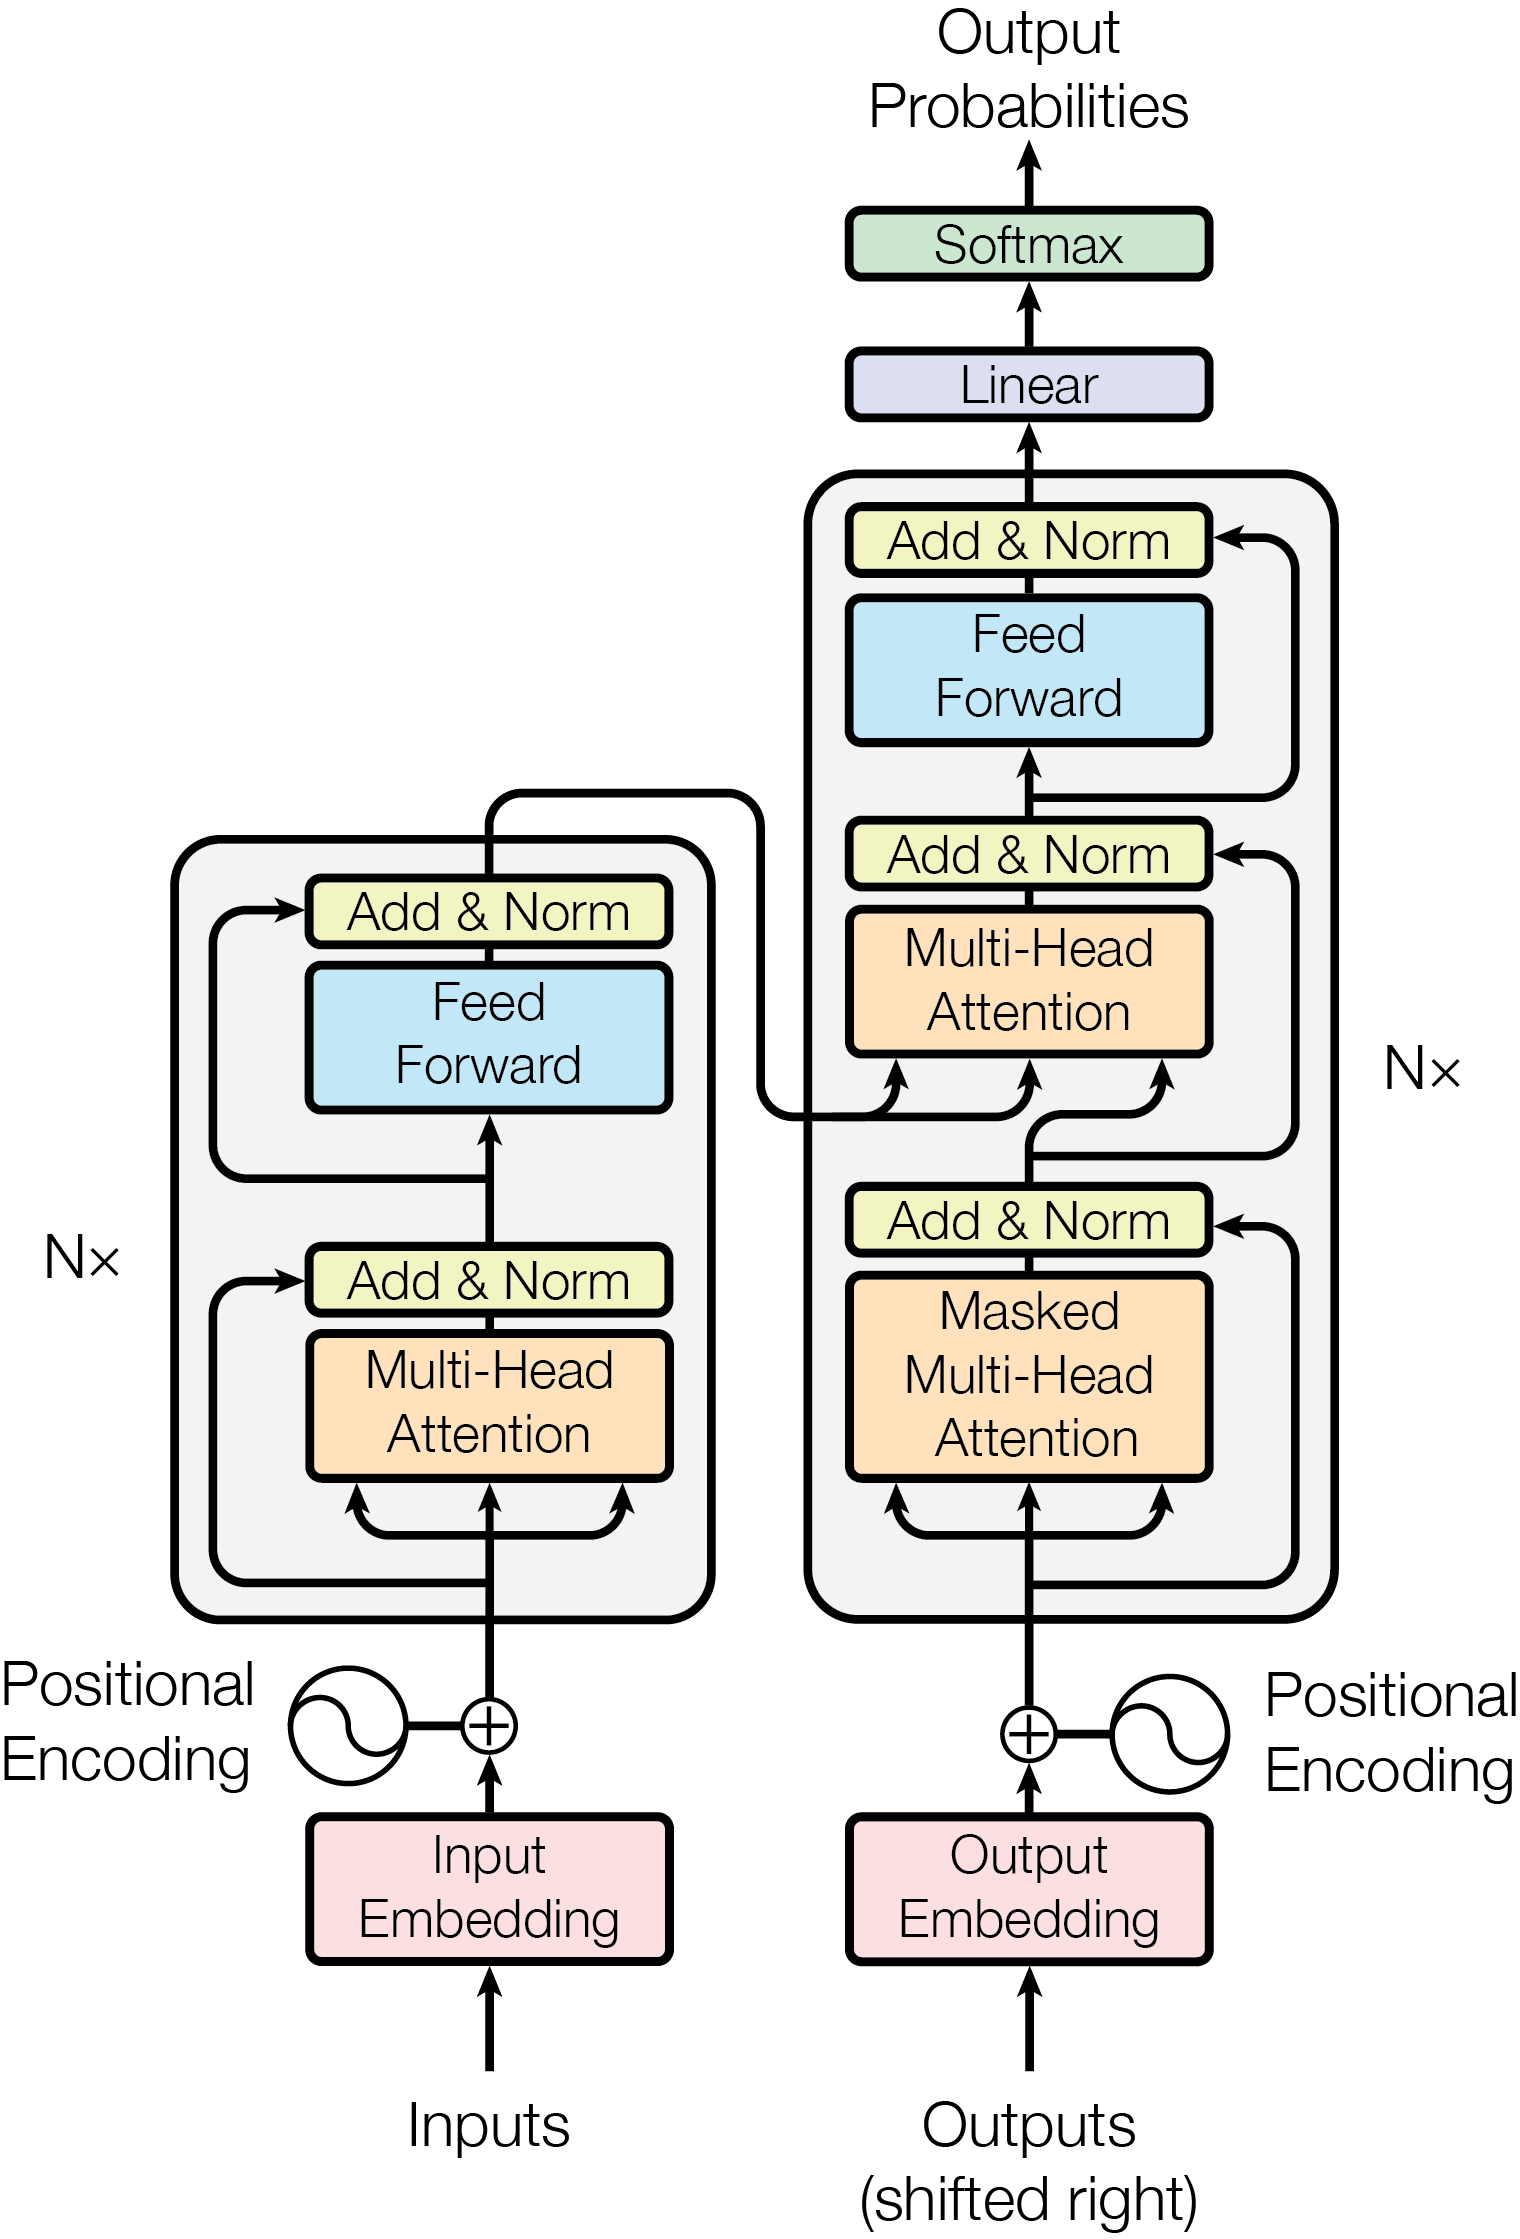
\includegraphics[width=0.5\linewidth]{figures/2_transformer} 

}

\caption{The original Transformer model architecture by \textcite{vaswani-etal-2017-attention}.}\label{fig:transformer}
\end{figure}

The original Transformer architecture comprises an encoder and a decoder, each composed of a stacked sequence of identical layers that transform input embeddings in outputs with the same dimension (hence the name). First, the encoder maps the sequence \((x_1, \dots, x_n)\) to a sequence of embeddings \(\boldsymbol z = (z_1, \dots, z_n)\). Given \(\boldsymbol z\), the decoder then autoregressively produces an output token sequence \((y_1, \dots, y_m)\). Each layer of the Transformer encoder comprises two sublayers, a \textbf{multi-head self-attention mechanism} and a \textbf{feed-forward network}, surrounded by residual connections and followed by layer normalization. The decoder includes a third layer that performs multi-head self-attention over the encoder output and modifies the original self-attention sublayer to prevent attending to future context, as required by the language modeling objective. Figure \ref{fig:transformer} presents the original architecture for a \(N\)-layer Transformer. I will now proceed to describe the main components of the Transformer model.

\paragraph{Positional Encodings} The original Transformer relies on two sets of embeddings to represent the input sequence: learned \textbf{word embeddings}, used as vector representations for each token in the vocabulary, and fixed \textbf{positional encodings} (PEs) used to inject information about the position of tokens in the sequence. Those are needed since no information about the sequential nature of the input would otherwise be preserved. For position \(pos\) and dimension \(i\), PEs correspond to sinusoidal periodic functions that were empirically shown to perform on par with learned embeddings, and were chosen to enable extrapolation for longer sequences:

\begin{align} 
PE_{pos, 2i} = \sin(\text{pos}/10000^{2i/|h|}) \\
PE_{pos, 2i + 1} = \cos(\text{pos}/10000^{2i/|h|})
\end{align}

where \(|h|\) is the model's hidden layer size. Embeddings and PEs are summed and passed to the attention layer.

\paragraph{Self-Attention} The \emph{scaled dot-product self-attention} mechanisms is the driving force of the Transformer architecture. Given an input embedding matrix \(X\), we multiply it by three weight matrices \(W^Q, W^K, W^V\) obtaining the projections \(Q\) (\textbf{queries}), \(K\) (\textbf{keys}) and \(V\) (\textbf{values}). Those are then combined by the self-attention function as follows:

\begin{equation}
\text{Attention(Q,K,V)} = \text{softmax}\Big ( \frac{QK^T}{\sqrt{d_k}}\Big)V
\end{equation}

where \(d_k\) is the size of individual query and key vectors. The output of this operation is a matrix \(Z\) which will be passed to the feed-forward layer. The self attention mechanism is further extended to \textbf{multi-head self-attention} in Transformer architectures. In the multi-head variant, the attention function is applied in parallel to \(n\) version of queries, keys and values projected with learned parameter matrices, and outputs are finally concatenated and projected again to obtain final values:

\begin{align}
\text{MultiHead}(Q,K,V) = \text{Concat}(\text{head}_1,\dots, \text{head}_n)W^O \\
\text{where } \text{head}_i = \text{Attention}(QW_i^Q,KW_i^K,VW_i^V)
\end{align}

Where \(W_i^Q \in \mathbb{R}^{|h| \times d_k}\), \(W_i^K \in \mathbb{R}^{|h| \times d_k}\), \(W_i^V \in \mathbb{R}^{|h| \times d_v}\) and \(W^O \in \mathbb{R}^{nd_v \times |h|}\). In multi-head attention layers of Figure \ref{fig:transformer}, each position can attend to all position from the previous layer, while in the \textbf{masked multi-head attention} layer only previous positions in the sequence can be attended by applying a triangular mask to attention matrices. This additional step is needed to preserve the autoregressive property during decoding.

\paragraph{Feed-forward Layer} Each block in the encoder and the decoder contains an independent fully connected 2-layer feed-forward network with a ReLU nonlinearity applied separately to each position of the sequence:

\begin{equation}
\text{FFN}(Z) = \max(0,Z\,\Theta_1 + b_1)\Theta_2 + b_2
\end{equation}

where \(Z\) are the representations passed forward from the attention sublayer, \(\Theta_1, \Theta_2\) are two learned independent parameter matrices for each layer and \(b_1, b_2\) are their respective bias vectors.

Now that the main concepts regarding the Transformer architecture have been introduced, the two Transformer-based models used in this study will be presented.

\paragraph{GPT-2} GPT-2 \autocite{radford-etal-2019-language} is a transformer model built using only the decoder blocks with masked self-attention, alongside BPE tokenization. The latter's autoregressive capabilities, i.e.~being able to iteratively add a newly predicted token to the existing sequence in the next steps, make it especially suitable for text generation and related tasks. The learning of model parameters is performed in two stages. First, an \textbf{unsupervised pretraining} is carried out to learn a high capacity language model on a large corpus: in particular, here the model is trained to maximize the likelihood of sequential language modeling over \textbf{WebText}, a corpus containing roughly 8 million documents (40GB of text), by adapting its parameters using stochastic gradient descent. The purpose of this step is to learn contextual word embeddings encoding both low and high-level information that can be recycled in downstream tasks, following the \textbf{transfer learning} approach inspired by the field of computer vision and initially proposed by \textcite{howard-ruder-2018-universal} for NLP. The second step is a \textbf{supervised fine-tuning}, where the language modeling softmax layer is replaced by a task-specific layer (called \textbf{head}) with parameters \(W_y\) receiving final transformer activations \(h_l\) and predicting a label \(y\) (e.g.~in a classification task) as:

\begin{equation}
P(y|x_1,\dots, x_m) = \text{softmax}(h^{sent}_lW_y)
\end{equation}

where \(h_l^{sent}\) is the sentence-level representation for \((x_1, \dots, x_m)\). The parameters of the whole model, including transformer blocks and task-specific heads, can then be tuned by minimizing the loss \(\mathcal{L}\) over the whole supervised corpus \(\mathcal{C}\):

\begin{equation}
\mathcal{L}(\mathcal{C}) = - \sum_{(x,y)} \log P(y|x_1, \dots, x_m) 
\end{equation}

Figure \ref{fig:gpt2} visualizes the forward pass through the GPT-2 architecture. We see from the figure that attention patterns learned during pre-trained are often interpretable. Here, the token \emph{it} is correctly identified as the pronoun referring to the subject \emph{a robot}. Authors show how large NLMs such as GPT-2 become strong unsupervised multitask learners when trained on sufficiently large corpora, providing the initial motivation for choosing pretrained Transformer models for experiments throughout this study. GPT-2 will be specifically be employed in the experiments of Chapter \ref{chap:ex3}, where its autoregressive nature is ideal for replicating human surprisal estimates during sequential reading on garden-path sentences.



\begin{figure}

{\centering 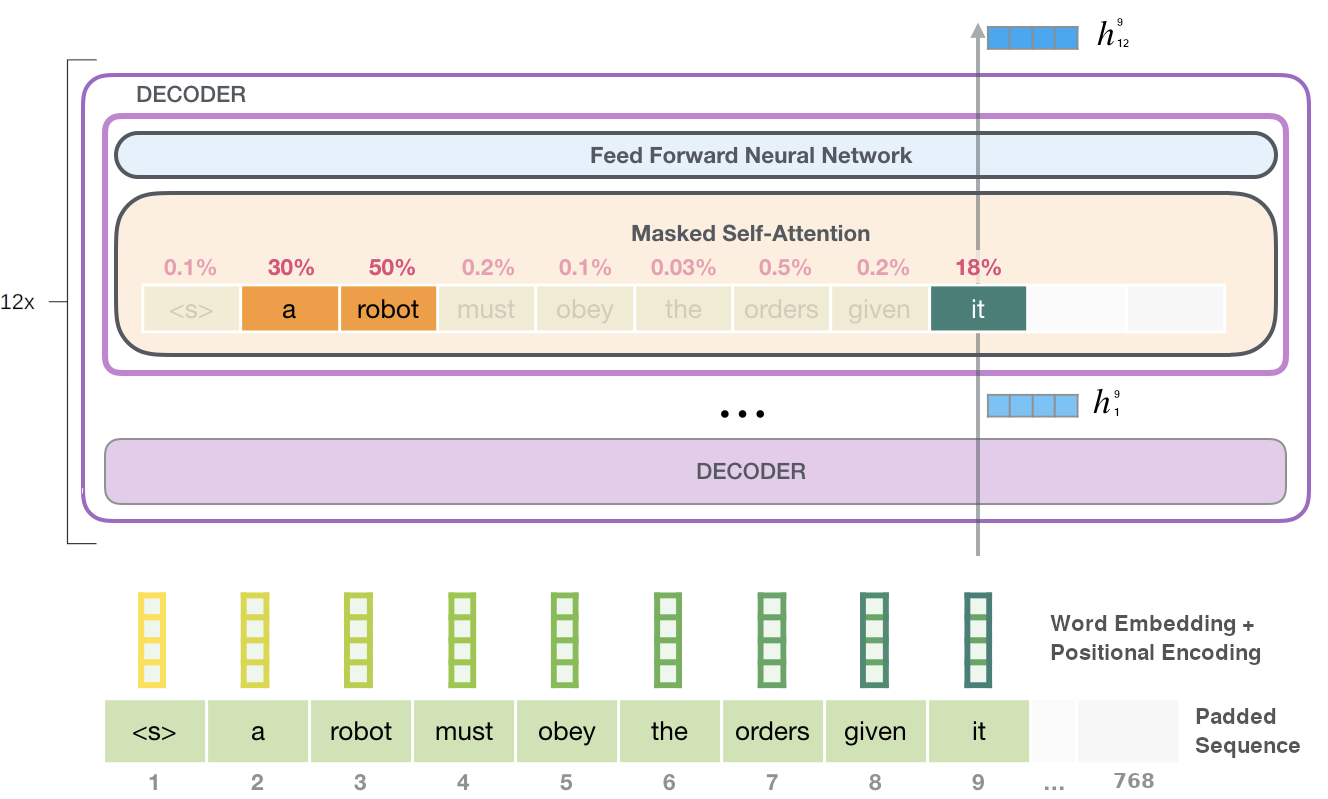
\includegraphics[width=1\linewidth]{figures/2_gpt2} 

}

\caption{An overview of the forward pass in GPT-2. Adapted from \textcite{alammar-2018-illustratedgpt2}.}\label{fig:gpt2}
\end{figure}

\paragraph{ALBERT} ALBERT \autocite{lan-etal-2020-albert} is an efficient variant of the Bidirectional Encoder Representations from Transformers (\textbf{BERT}) approach by \textcite{devlin-etal-2019-bert}. BERT was built following the intuition that many sentence-level tasks would greatly benefit from an approach capable of incorporating bidirectional context inside language representations. This is not the case for decoder-based approaches like GPT-2 that, being aimed at generation-oriented tasks, could only leverage the previous context using masked self-attention. BERT tackles the unidirectional constraint by introducing \textbf{masked language modeling} (MLM, see Equation \eqref{eq:sent-surprisal-cases}) and using a stack of transformer encoder layers with GELU nonlinearities \autocite{hendrycks-gimpel-2016-gaussian}.

As for GPT-2, the pretraining and fine-tuning steps are taken to provide the model with general language knowledge and subsequently adapt it to specific downstream tasks. At each pretraining step, a fixed portion of input tokens get masked, and the model predicts the original vocabulary id of masked tokens. Moreover, a sentence-level task is used to improve discourse coherence. For BERT, the \textbf{next sentence prediction} (NSP) task is adopted, i.e.~determining whether, given two sentences, they are consecutive or not in the original text using both positive and negative pairs. NSP was found unreliable by subsequent studies and was replaced in ALBERT by a \textbf{sentence ordering prediction} loss that is more challenging for the model. A third set of \textbf{segment embeddings} is added to initial representations to distinguish input sentences in multi-sentence tasks. Special tokens \texttt{{[}CLS{]}} and \texttt{{[}SEP{]}} are added as sentence-level representations.

ALBERT introduces two main contributions aimed at reducing the final number of model parameters inside BERT:

\begin{itemize}
\item
  \textbf{Factorized embedding parametrization}: a projection layer is introduced between the embedding matrix \(E\) and the hidden layer \(H\) of the model so that the dimensions of the two are untied. This approach modifies embedding parameter count from \(O(|V| \times |E|)\) to \(O(|\mathcal{V}| \times |E| + |E| \times |h|)\), with \(|\mathcal{V}|, |E|, |h|\) being respectively the sizes of vocabulary, embedding vectors and hidden layers. A significant reduction in model parameters is therefore produce when \(|h| \gg |E|\), which is desirable since \(H\) contains \emph{context-dependent representations} that encode more information than the \emph{context-independent} ones of \(E\).
\item
  \textbf{Cross-layer parameter sharing}: All layers of ALBERT share the same set of feed-forward and self-attention parameters. Therefore, we can see ALBERT as an iterated function \(f_A^n: h \rightarrow h'\), where \(n\) is the number of encoder layers present in the model (in this study \(n=12\)), with parameters trained using end-to-end stochastic gradient descent.
\end{itemize}

Both factors significantly contribute to reducing the computational complexity of the model without affecting too much its performances: the ALBERT base used in all experimental chapters of this study have 9x fewer parameters than a regular BERT base model (12M vs.~108M) while performing comparably well on many natural language understanding benchmarks such as GLUE \autocite{wang-etal-2018-glue} and SQuAD \autocite{rajpurkar-etal-2016-squad}.

Figure \ref{fig:albert} presents how a pretrained ALBERT model can be leveraged for sentence classification, using the ARA task as an example. We note that the procedure is the same as for GPT-2: a task-specific classification head is initialized with random weights, and the whole model-head architecture is fine-tuned on the target task end-to-end. The figure also shows how the common choice for BERT-based models is to use their \texttt{{[}CLS{]}} token \(h_{12}^{1}\) as the full-sentence representation equivalent \(h_{12}^{sent}\).



\begin{figure}

{\centering 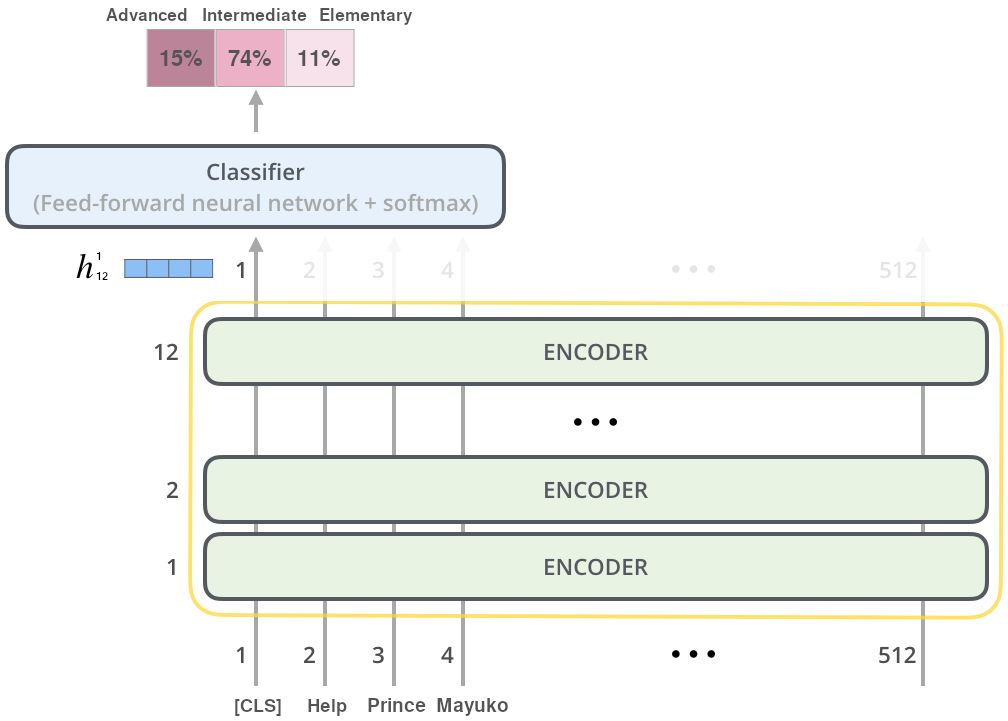
\includegraphics[width=0.85\linewidth]{figures/2_albert} 

}

\caption{Using a pretrained ALBERT model for the ARA task. Adapted from \textcite{alammar-2018-illustratedbert}.}\label{fig:albert}
\end{figure}

To conclude, the fine-tuning approach relying on a pretrained model ``body'' and a task-specific head adopted in both GPT-2 and ALBERT can be extended out-of-the-box to a \textbf{multitask learning} scenario. A multitask approach can prove useful when considering parallel annotations on the same corpus that provide similar but complementary information about a studied phenomenon's nature. We can interpret this as an inductive bias that encourages finding knowledge representations to explain multiple sets of annotations at once.\footnote{See \textcite{ruder-2017-overview} for a comprehensive overview} More specifically, multitask learning with \textbf{hard parameter sharing} \autocite{caruana-1997-multitask} is performed in all experimental sections over eye-tracking scores to produce representations encompassing the whole set of phenomena related to natural reading. For doing so, each metric was associated with a task-specific head, and the whole set of heads was trained while sharing the same underlying model.

\hypertarget{subsubchap:syntax-nlm}{%
\subsection{Emergent Linguistic Structures in Neural Language Models}\label{subsubchap:syntax-nlm}}

This section presents evidence in support of the ability of pretrained language models to effectively encode language-related properties in their learned representations.\footnote{\textcite{rogers-etal-2020-primer} and \textcite{linzen-baroni-2021-syntactic} are surveys covering this topic.}

\textcite{lin-etal-2019-open} were among the first to highlight how BERT representations encode hierarchical structures akin to syntax trees, despite the absence of syntactic information or recurrent biases during pretraining. \textcite{liu-etal-2019-linguistic} and \textcite{tenney-etal-2019-bert} further showed that contextualized embeddings produced by BERT encode information about part-of-speech, entity roles, and partial syntactic structures.

\textcite{hewitt-manning-2019-structural} formulate the \textbf{syntax distance hypothesis}, assuming that there exists a linear transformation \(B\) of the word representation space under which vector distance encodes parse trees. They proceed to test this assumption equating L2 distance in the 2-dimensional space of representations projected by \(B \in \mathbb{R}^{2 \times |h|}\) and tree distances in parse trees, finding a close match between BERT representational space and Penn Treebank formalisms. The approach is visualized in Figure \ref{fig:struct-probe}. \textcite{jawahar-etal-2019-bert} work support these findings, highlighting a close match between BERT representation and dependency trees after testing multiple decomposition schemes. The syntax distance hypothesis's validity is especially relevant to this work, given the aforementioned importance of syntactic properties in driving human subjects' perception of complexity.



\begin{figure}

{\centering 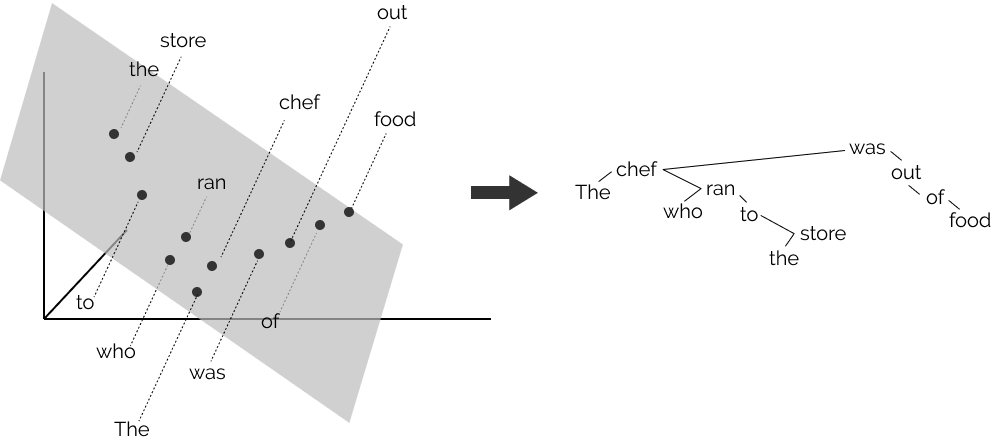
\includegraphics[width=0.85\linewidth]{figures/2_struct_probe} 

}

\caption{The mapping from 2D representation space to syntax tree distances adopted in \textcite{hewitt-manning-2019-structural}.}\label{fig:struct-probe}
\end{figure}

Despite the evidence of syntactic knowledge in contextual word representations, recent results suggest that the model may not leverage this for its predictions. \textcite{ettinger-2020-bert} highlights the insensitivity of BERT to negation and malformed inputs using psycholinguistic diagnostics commonly used with human subjects, while \textcite{wallace-etal-2019-nlp} show that nonsensical inputs do not affect the prediction quality of BERT, despite having a clear input on underlying syntactic structures. These results are coherent with the experimental findings of this study and will be further discussed in later sections.

\hypertarget{subchap:analyzing-nlm}{%
\section{Analyzing Neural Models of Complexity}\label{subchap:analyzing-nlm}}

Having introduced the model architectures that will be used throughout this study, we will now focus on the interpretability approaches allowing us to analyze and compare neural network representations.

When training deep neural networks, we would like to go beyond predictive performance and understand how different design choices and training objectives affect learned representations from a qualitative viewpoint. This fact is especially crucial in the model-driven approach adopted in this work, as stated at the end of Section \ref{subchap:desiderata}. While for linear models, the direct correspondence between the magnitude of feature coefficients and feature importance provides us with some out-of-the-box insights about decision boundaries and feature importance, the hierarchical and nonlinear structure that characterizes neural networks produce model weights that are relatively uninformative when taken in isolation.

This work focuses on two interpretability perspectives: highlighting linguistic knowledge encoded in model representations (Chapter \ref{chap:ex1}) and comparing representations across models trained on different complexity-related tasks (Chapter \ref{chap:ex2}). For the first objective, \emph{probing classifiers}, which have become the de-facto standard in the interpretability literature, are used to evaluate the amount of information encoded in each layer of the model.\footnote{See \textcite{belinkov-glass-2019-analysis} survey and \textcite{belinkov-etal-2020-interpretability} tutorial.} In the second case, two multivariate statistical analysis methods, namely \emph{representational similarity analysis} and \emph{canonical correlation analysis}, are leveraged to quantify the relation between model embeddings by evaluating their second-order similarity and learning a mapping to a shared low-dimensional space, respectively. The following sections conclude the chapter by presenting the three approaches in detail.

\hypertarget{subsubchap:probe}{%
\subsection{Probing classifiers}\label{subsubchap:probe}}

The \textbf{probing task approach} is a natural way to estimate the mutual information shared by a neural network's parameters and some latent property that the model could have implicitly learned during training. During probing experiments, a supervised model (\emph{probe}) is trained to predict the latent information from the network's learned representations. If the probe does well, we may conclude that the network effectively encodes some knowledge related to the selected property.

Formally speaking, let \(f: x_i \rightarrow y_i\) be a neural network model mapping a corpus of input sentences \(X = (x_1, \dots, x_n)\) to a set of outputs \(Y = (y_1, \dots, y_n)\). Assume that each sentence \(x_i\) is also labeled with some linguistic annotations \(z_i\), reflecting the underlying properties we aim to detect. Let also \(h_l(x_i)\) be the network's output at the \(l\)-th layer given the sentence \(x_i\) as input. To estimate the quality of representations \(h_l\) with respect to property \(z\), a supervised model \(g: h_l(x_i) \rightarrow z_i\) mapping representations to property values is trained. We take such model's performances as a proxy of \(H(h_l(x),z)\). In information theoretic terms, the probe is trained to minimize entropy \(H(z|h_l(x))\), and by doing that it maximizes mutual information between the two quantities.

The probe \(g\) does not need to be a linear model. While historically simple linear probes were used to minimize the risk of memorization, recent results show that more complex probes produce tighter estimates for the actual underlying information \autocite{pimentel-etal-2020-information}. To account for the probe's ability to learn the task through sheer memorization, \textcite{hewitt-liang-2019-designing} introduce \emph{control tasks} using the performances of a probe exposed to random labels as baselines.

\textcite{alain-bengio-2016-understanding} were among the first to use linear probing classifiers as tools to evaluate the presence of task-specific information inside neural networks' layers. The approach was later extended to the field of NLP by \textcite{conneau-etal-2018-cram} and \textcite{zhang-bowman-2018-language} \emph{inter alia}, which evaluated the presence of semantic and syntactic information inside sentence embeddings generated by LSTM encoders \autocite{hochreiter-1997-long} pretrained on different objectives using probing task suites. Recently, \textcite{miaschi-dellorletta-2020-contextual} showed how contextual representations produced by pretrained Transformer models could encode sentence-level properties within single-word embeddings. Moreover, \textcite{miaschi-etal-2020-linguistic} highlighted the tendency of pretrained NLMs to lose general linguistic information during the fine-tuning process and found a positive relation between encoded linguistic information and the downstream performances of the model.

\hypertarget{subsubchap:rsa}{%
\subsection{Representational Similarity Analysis}\label{subsubchap:rsa}}



\begin{figure}

{\centering 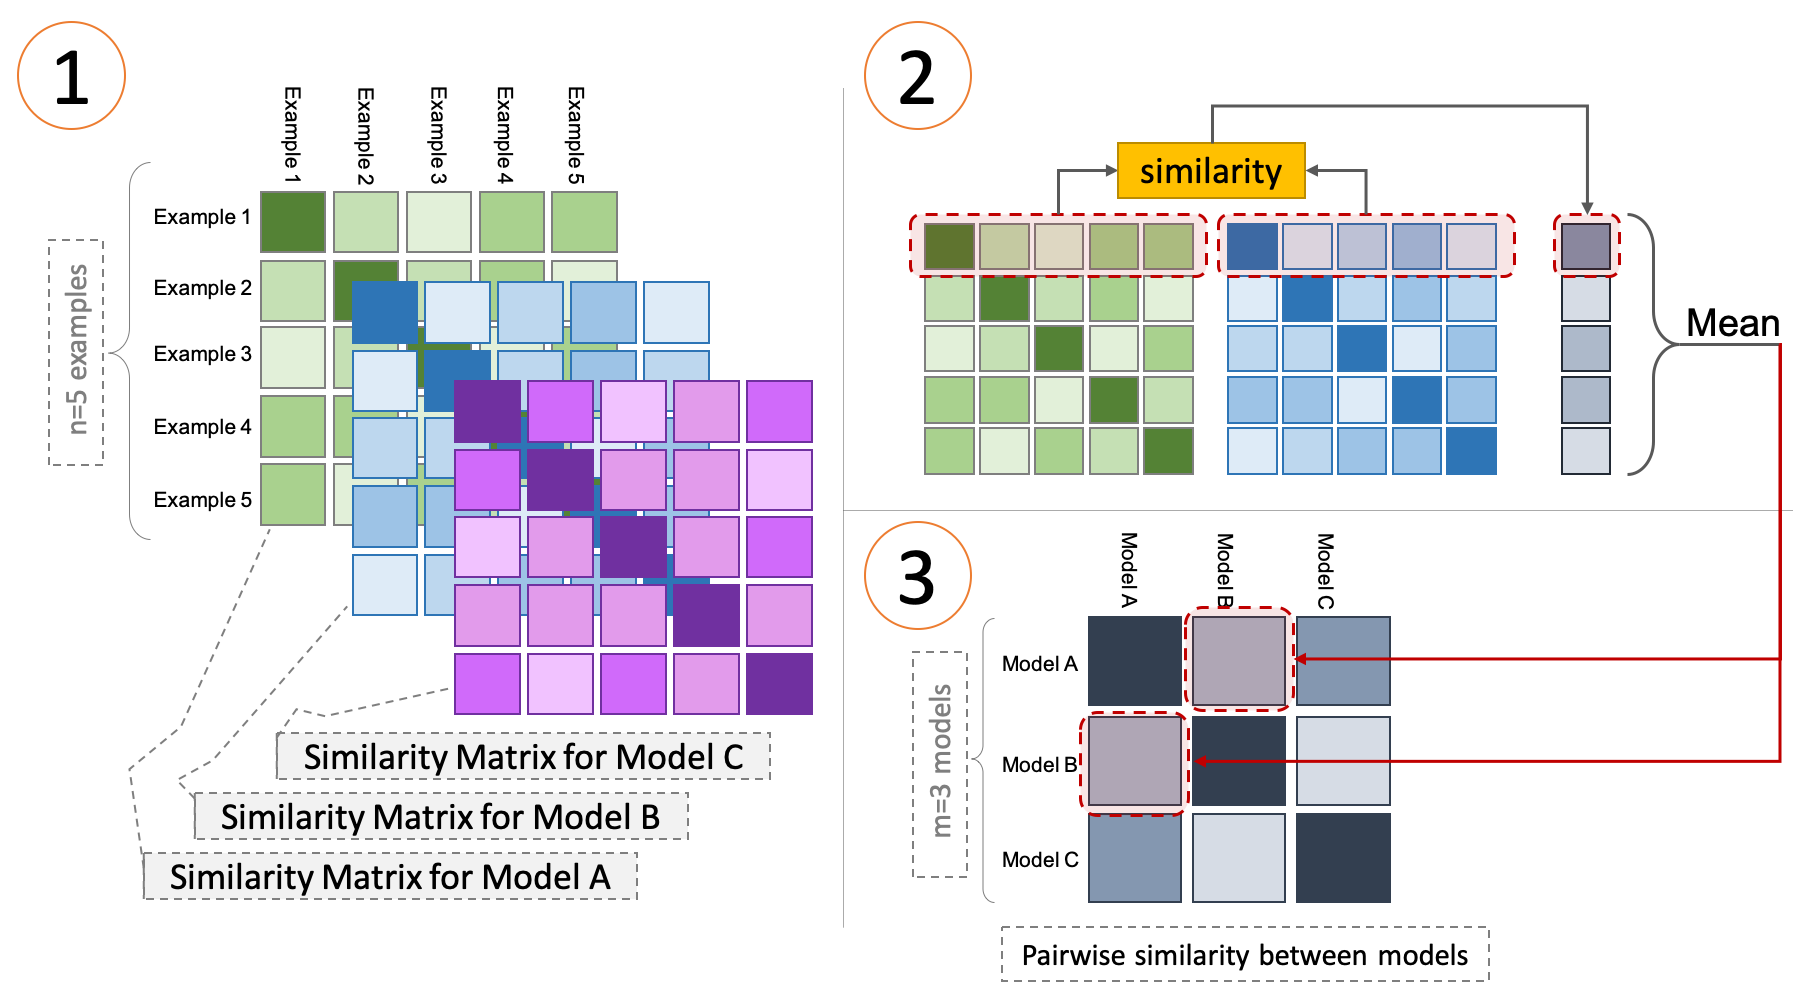
\includegraphics[width=1\linewidth]{figures/2_rsa} 

}

\caption{The Representational Similarity Analysis (RSA) algorithm applied to the representations of three models. Image taken from \textcite{abnar-2020-visualization}.}\label{fig:rsa}
\end{figure}

\textbf{Representational similarity analysis} (RSA, \textcite{laakso-2000-content}) is a technique developed in the field of cognitive science to evaluate the similarity of fMRI responses in selected regions of the brain after a stimulus \autocite{kriegeskorte-etal-2008-representational}. The technique can be extended to compare the heterogeneous representational spaces formed by a set of computational models \(m\) exposed to a shared set of observations. Figure \ref{fig:rsa} visualizes the approach. First, each model is fed with a shared corpus of \(n\) sentences to produce a set of matrix embeddings \((E^1, \dots, E^m)\), where \(E^i_j\) represents the embedding produced by the last layer of the \(i\)-th model on the \(j\)-th sentence of the corpus.\footnote{This can be any layer; embeddings can be produced by different layers of the same model.} Next, for each matrix \(E^i\) a representational distance matrix \(S^i\) is produced such that \(S^i_{j,k} = \text{sim}(E^i_j, E^i_k),\;S^i \in \mathbb{R}^{n \times n}\) where \(\text{sim}_1\) is a similarity function (here, \emph{dot product}). \(S_i\) encodes information on the similarity subsisting between model activations across different observations. Finally, a second-level \emph{representational similarity matrix} \(S'\) is computed, where for each pair of matrices \((S^i, S^j)\) the corresponding \(S'_{i,j}\) entry has value:

\begin{equation}
S'_{i,j} = S'_{j,i} = \frac{1}{n}\sum_{k=1}^n \text{sim}_2\big(\,\eta\,(S^i_k),\eta\,(S^j_k)\big)
\end{equation}

where \(\eta\) is the L1 normalization function and \(\text{sim}_2\) is a similarity function (here, \emph{Pearson's correlation coefficient}). Each entry \(S'_{i,j}\) corresponds to a similarity score between activity patterns of model \(i\) and model \(j\) across the entire set of \(n\) observations.

In the context of NLP, \textcite{abnar-etal-2019-blackbox} recently used RSA to compare the activations of multiple neural language models and evaluated the impact of parameter values on the representations formed by a single model. Interestingly, they also use RSA to compare fMRI imaging data collected from human subjects and NLMs activations. \textcite{abdou-etal-2019-higher} use RSA to highlight the connection between processing difficulties (measured by high gaze metrics values) and the representational divergence, both inter and intra-encoder. \textcite{abnar-etal-2020-transferring} visualize training paths of various neural network architectures as 2D projections of RSA and show how different inductive biases can be transferred across network categories using knowledge distillation \autocite{hinton-etal-2015-distilling}.

\hypertarget{subsubchap:pwcca}{%
\subsection{Projection-Weighted Canonical Correlation Analysis}\label{subsubchap:pwcca}}

\textbf{Canonical correlation analysis} (CCA, \textcite{thompson-1984-canonical}) is a statistical technique for relating two sets of observations arising from an underlying unknown process. In the context of this work, the underlying process is represented by NLMs being trained on complexity-related tasks. Given a corpus of sentences \(X = (x_1, \dots, x_m)\) annotated with complexity labels, we have that \(\boldsymbol z^l_ = (z_i^l(x_1), \dots z_i^l(x_m))\) corresponds to all activations of neuron \(z_i\) at layer \(l\) stacked to form a vector.\footnote{Different from the activation vector, i.e.~all neurons' activations for a single input \((z^l_1(x_1),\dots,z^l_n(x_1))\)} If we consider all activations of all neurons in a layer \(L_i = (z^i_1, \dots, z^i_n)\) for all inputs, we can represent them as a matrix \(A_i \in \mathbb{R}^{m \times n}\), i.e.~a set of multidimensional variates where \(n\) is the number of neurons in the layer. The CCA algorithm aims to \emph{identify the best} (i.e.~most correlated) \emph{linear relationship under mutual orthogonality and norm constraints between two sets of multidimensional variates}, which in this case are activation matrices like \(L_1\). This approach was used, among other things, to study the coherence between modeled and real brain activations \autocite{sussillo-etal-2015-neural}.

Formally, if we have two activation matrices \(A_1, A_2 \in \mathbb{R}^{m \times n}\) we aim to find vectors \(w, v \in \mathbb{R}^m\) such that the correlation:

\begin{equation}
\rho = \frac{\langle w^TA_1, v^TA_2 \rangle}{\|w^TA_1\| \cdot \| v^T A_2\|}
\end{equation}

is maximized. The formula can be solved by changing the basis and recurring to singular value decomposition. The output of CCA is a set of singular pairwise orthogonal vectors \(u, v\) and their canonical correlation coefficients \(\rho \in [0,1]\) representing the correlation of vectors \(w^TA_1\) and \(v^TA_2\).



\begin{figure}

{\centering 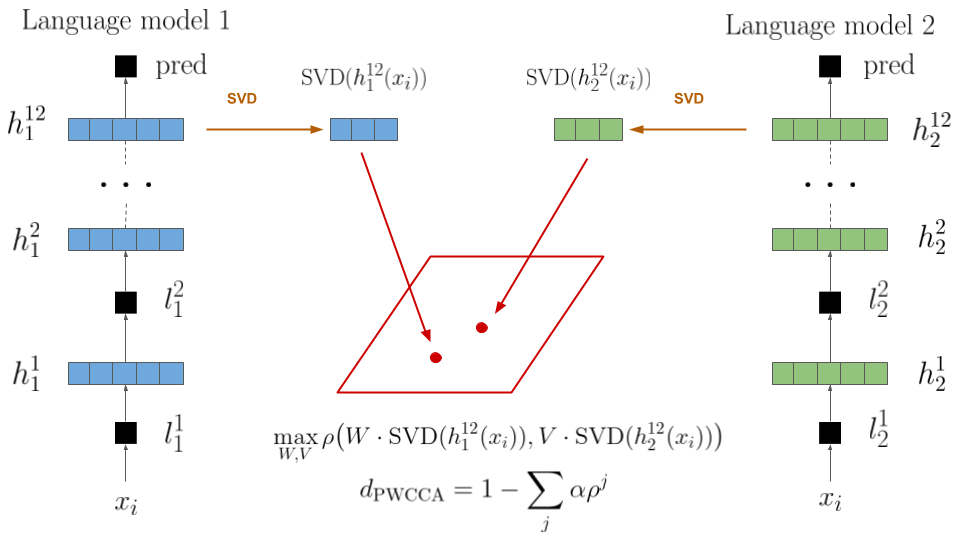
\includegraphics[width=0.85\linewidth]{figures/2_pwcca} 

}

\caption{Projection-Weighted Canonical Correlation Analysis (PWCCA) applied to last-layer representations of two language models.}\label{fig:pwcca}
\end{figure}

The SVCCA method \autocite{guyon-etal-2017-svcca} extends the CCA approach for deep learning research by pruning neurons through a singular value decomposition step before computing canonical correlation coefficients. As the authors mention, ``This is especially important in neural network representations, where as we will show many low variance directions (neurons) are primarily noise''. Then, the similarity between two layers \(L_1, L_2\) is computed as the mean correlation coefficient produce by SVCCA, and adapted to a distance measure for evaluation:
\begin{equation}
d_{\text{SVCCA}}(A_1, A_2) = 1 - \frac{1}{|\rho|} \sum_{i=1}^{|\rho|} \rho^{(i)}
\end{equation}
\textcite{morcos-etal-2018-insights} suggest that the equal importance given to all the \(|\rho|\) SVCCA vectors during the final averaging step may be problematic since it has been extensively shown that overparametrized neural networks often do not recur to their full dimensionality for representing solutions \autocite{frankle-carbin-2018-lottery}. They suggest replacing the mean with a weighted mean:
\begin{equation}
d_{\text{PWCCA}}(A_1, A_2) = 1 - \sum_{i=1}^{|\rho|} \alpha \rho^{(i)} \;\;\text{with} \;\; \tilde \alpha_i = \sum_j |\langle h_i, x_j \rangle|
\end{equation}
where weights \(\alpha\) corresponds to the portion of inputs \(x\) accounted for by CCA vectors \(h\) and \(\tilde \alpha_i\) values are normalized such that \(\sum_i \alpha_i = 1\). The resulting approach, \emph{projection-weighted canonical correlation analysis} (PWCCA), is used in this study and was shown to be much more robust than SVCCA to filter noise in activations. Figure \ref{fig:pwcca} visualizes the selected approach.

Notable applications of CCA-related methods in NLP are \textcite{saphra-lopez-2019-understanding}, where SVCCA is used to study the evolution of LSTM language models' representations during training, and \textcite{voita-etal-2019-bottom}, where PWCCA is used to compare Transformer language models across layers and pretraining objectives.

\titlespacing{\chapter}{0pt}{0pt}{35pt}

\hypertarget{chap:ex1}{%
\chapter{\texorpdfstring{\textbf{Complexity Phenomena in Linguistic Annotations and Language Models}}{Complexity Phenomena in Linguistic Annotations and Language Models}}\label{chap:ex1}}

\minitoc 

\chaptermark{Complexity Phenomena in Linguistic Annotations and Language Models}

\begin{quote}
This chapter investigates the relationship between online gaze metrics and offline perceived complexity judgments by studying how the two viewpoints are represented by a neural language model trained on human-produced data. First, a preliminary analysis of linguistic phenomena associated with the two complexity viewpoints is performed, highlighting similarities and differences across metrics. The effectiveness of a regressor based on explicit linguistic features is then evaluated for sentence complexity prediction and compared to the results obtained by a fine-tuned neural language model with contextual representations. In conclusion, the linguistic competence inside the language model's embeddings is probed before and after fine-tuning, showing how linguistic information encoded in representations changes as the model learns to predict complexity.
\end{quote}

Given the conceptual similarity between raw cognitive processing and human perception of complexity, this chapter investigates whether the relation between eye-tracking metrics and complexity judgments can be highlighted empirically in human annotations and language model representations. With this aim, linguistic features associated with various sentence-level structural phenomena are analyzed in terms of their correlation with offline and online complexity metrics. The performance of models using either complexity-related explicit features or contextualized word embeddings is evaluated, focusing mainly on the neural language model ALBERT \autocite{lan-etal-2020-albert} introduced in Section \ref{subchap:nlm}. The results highlight how both explicit features and learned representations obtain comparable performances when predicting complexity scores. Finally, the focus is shifted to studying how complexity-related properties are encoded in the representations of ALBERT.

This perspective goes in the direction of exploiting human processing data to address the interpretability issues of unsupervised language representations \autocites{hollenstein-etal-2019-cognival}{gauthier-levy-2019-linking}{abnar-etal-2019-blackbox}, leveraging the \emph{probing task} approach introduced in Section \ref{subsubchap:probe}. It is observed that online and offline complexity fine-tuning produces a consequent increase in probing performances for complexity-related features during probing experiments. This investigation has the specific purpose of studying whether and how learning a new task affects the linguistic properties encoded in pretrained representations. While pre-trained models have been widely studied using probing methods, the effect of fine-tuning on encoded information was seldom investigated. To my best knowledge, no previous work has taken into account sentence complexity assessment as a fine-tuning task for NLMs. Results suggest that the model's abilities during training are interpretable from a linguistic perspective and are possibly related to its predictive capabilities for complexity assessment.

\paragraph{Contributions} This is the first work displaying the connection between online and offline complexity metrics and studying how a neural language model represents them. This work:

\begin{itemize}
\item
  Provides a comprehensive analysis of linguistic phenomena correlated with eye-tracking data and human perception of complexity, addressing similarities and differences from a linguistically-motivated perspective across metrics and at different levels of granularity;
\item
  Compares the performance of models using both explicit features and unsupervised contextual representations when predicting online and offline sentence complexity; and
\item
  Shows the natural emergence of complexity-related linguistic phenomena in the representations of language models trained on complexity metrics.\footnote{Code available at \url{https://github.com/gsarti/interpreting-complexity}}
\end{itemize}

\hypertarget{subchap:ex1-data}{%
\section{Data and Preprocessing}\label{subchap:ex1-data}}

The experiments of this chapter leverage two corpora, each capturing different aspects of linguistic complexity:

\paragraph{Eye-tracking} For online complexity metrics, only the monolingual English portion of GECO \autocite{cop-etal-2017-presenting}, presented in Section \ref{subsubchap:eye-tracking}, was used. Four online metrics spanning multiple phases of cognitive processing are selected, respectively: \emph{first pass duration} (FPD), \emph{total fixation count} (FXC), \emph{total fixation duration} (TFD) and \emph{total regression duration} (TRD) (see Table \ref{tab:et-metrics} for more details). Metrics are sum-aggregated at sentence-level and averaged across participants to obtain a single label for each metric-sentence pair. As a final step to make the corpus more suitable for linguistic complexity analysis, all utterances with fewer than five words, deemed uninteresting from a cognitive processing perspective, are removed.

\paragraph{Perceived Complexity} For the offline evaluation of sentence complexity, the English portion of the corpus by \textcite{brunato-etal-2018-sentence} was used (Section \ref{subsubchap:pc}). Sentences in the corpus have uniformly-distributed lengths ranging between 10 and 35 tokens. Each sentence is associated with 20 ratings of perceived-complexity on a 1-to-7 point scale. Duplicates and sentences for which less than half of the annotators agreed on a score in the range \(\mu_n \pm \sigma_n\), where \(\mu_n\) and \(\sigma_n\) are respectively the average and standard deviation of all annotators' judgments for sentence \(n\) were removed to reduce noise coming from the annotation procedure. Again, scores are averaged across annotators to obtain a single metric for each sentence.

Table \ref{tab:ex1-stats} presents an overview of the two corpora after preprocessing. The resulting eye-tracking (ET) corpus contains roughly four times more sentences than the perceived complexity (PC) one, with shorter words and sentences on average. The differences in sizes and domains between the two corpora account for multi-genre linguistic phenomena in the following analysis.

\begin{table}

\caption{\label{tab:ex1-stats}Descriptive statistics of the two sentence-level corpora after the preprocessing procedure.}
\centering
\fontsize{11}{13}\selectfont
\begin{tabular}[t]{l>{\centering\arraybackslash}p{10em}>{\centering\arraybackslash}p{12em}}
\toprule
\textbf{} & \textbf{Perceived Complexity} & \textbf{Eye-tracking (GECO)}\\
\midrule
labels & PC & FPD, FXC, TFD, TRD\\
\hline
domain(s) & financial news & literature\\
\hline
aggregation steps & avg. annotators & sentence sum-aggregation + avg. participants\\
\hline
filtering steps & filtering by agreement + remove duplicates & min. length > 5\\
\hline
\# of sentences & 1115 & 4041\\
\# of tokens & 21723 & 52131\\
avg. sent. length & 19.48 & 12.9\\
avg. token length & 4.95 & 4.6\\
\hline
\addlinespace[0.3em]
\multicolumn{3}{l}{\textbf{Length-binned subsets (\# of sentences)}}\\
\hspace{1em}Bin 10±1 size & 173 & 899\\
\hspace{1em}Bin 15±1 size & 163 & 568\\
\hspace{1em}Bin 20±1 size & 164 & 341\\
\hspace{1em}Bin 25±1 size & 151 & 215\\
\hspace{1em}Bin 30±1 size & 165 & 131\\
\hspace{1em}Bin 35±1 size & 147 & 63\\
\bottomrule
\end{tabular}
\end{table}

\hypertarget{subchap:ex1-analysis}{%
\section{Analysis of Linguistic Phenomena}\label{subchap:ex1-analysis}}

As a first step to investigate the connection between the two complexity paradigms, the correlation of online and offline complexity labels with various linguistic phenomena is evaluated. The Profiling-UD tool \autocite{brunato-etal-2020-profiling} introduced in Section \ref{subsubchap:structural} is used to annotate each sentence in our corpora and extract from it \textasciitilde{}100 features representing their linguistic structure according to the Universal Dependencies formalism \autocite{nivre-etal-2016-universal}. These features capture a comprehensive set of phenomena, from basic information (e.g.~sentence and word length) to more complex aspects of sentence structure (e.g.~parse tree depth, verb arity), including properties related to sentence complexity at different levels of description. A summary of the most relevant features is presented in Appendix \ref{app:ling-feats}. Features are ranked using their Spearman's correlation score with complexity metrics, and scores are leveraged to highlight the relation between linguistic phenomena and complexity paradigms.



\begin{figure}

{\centering 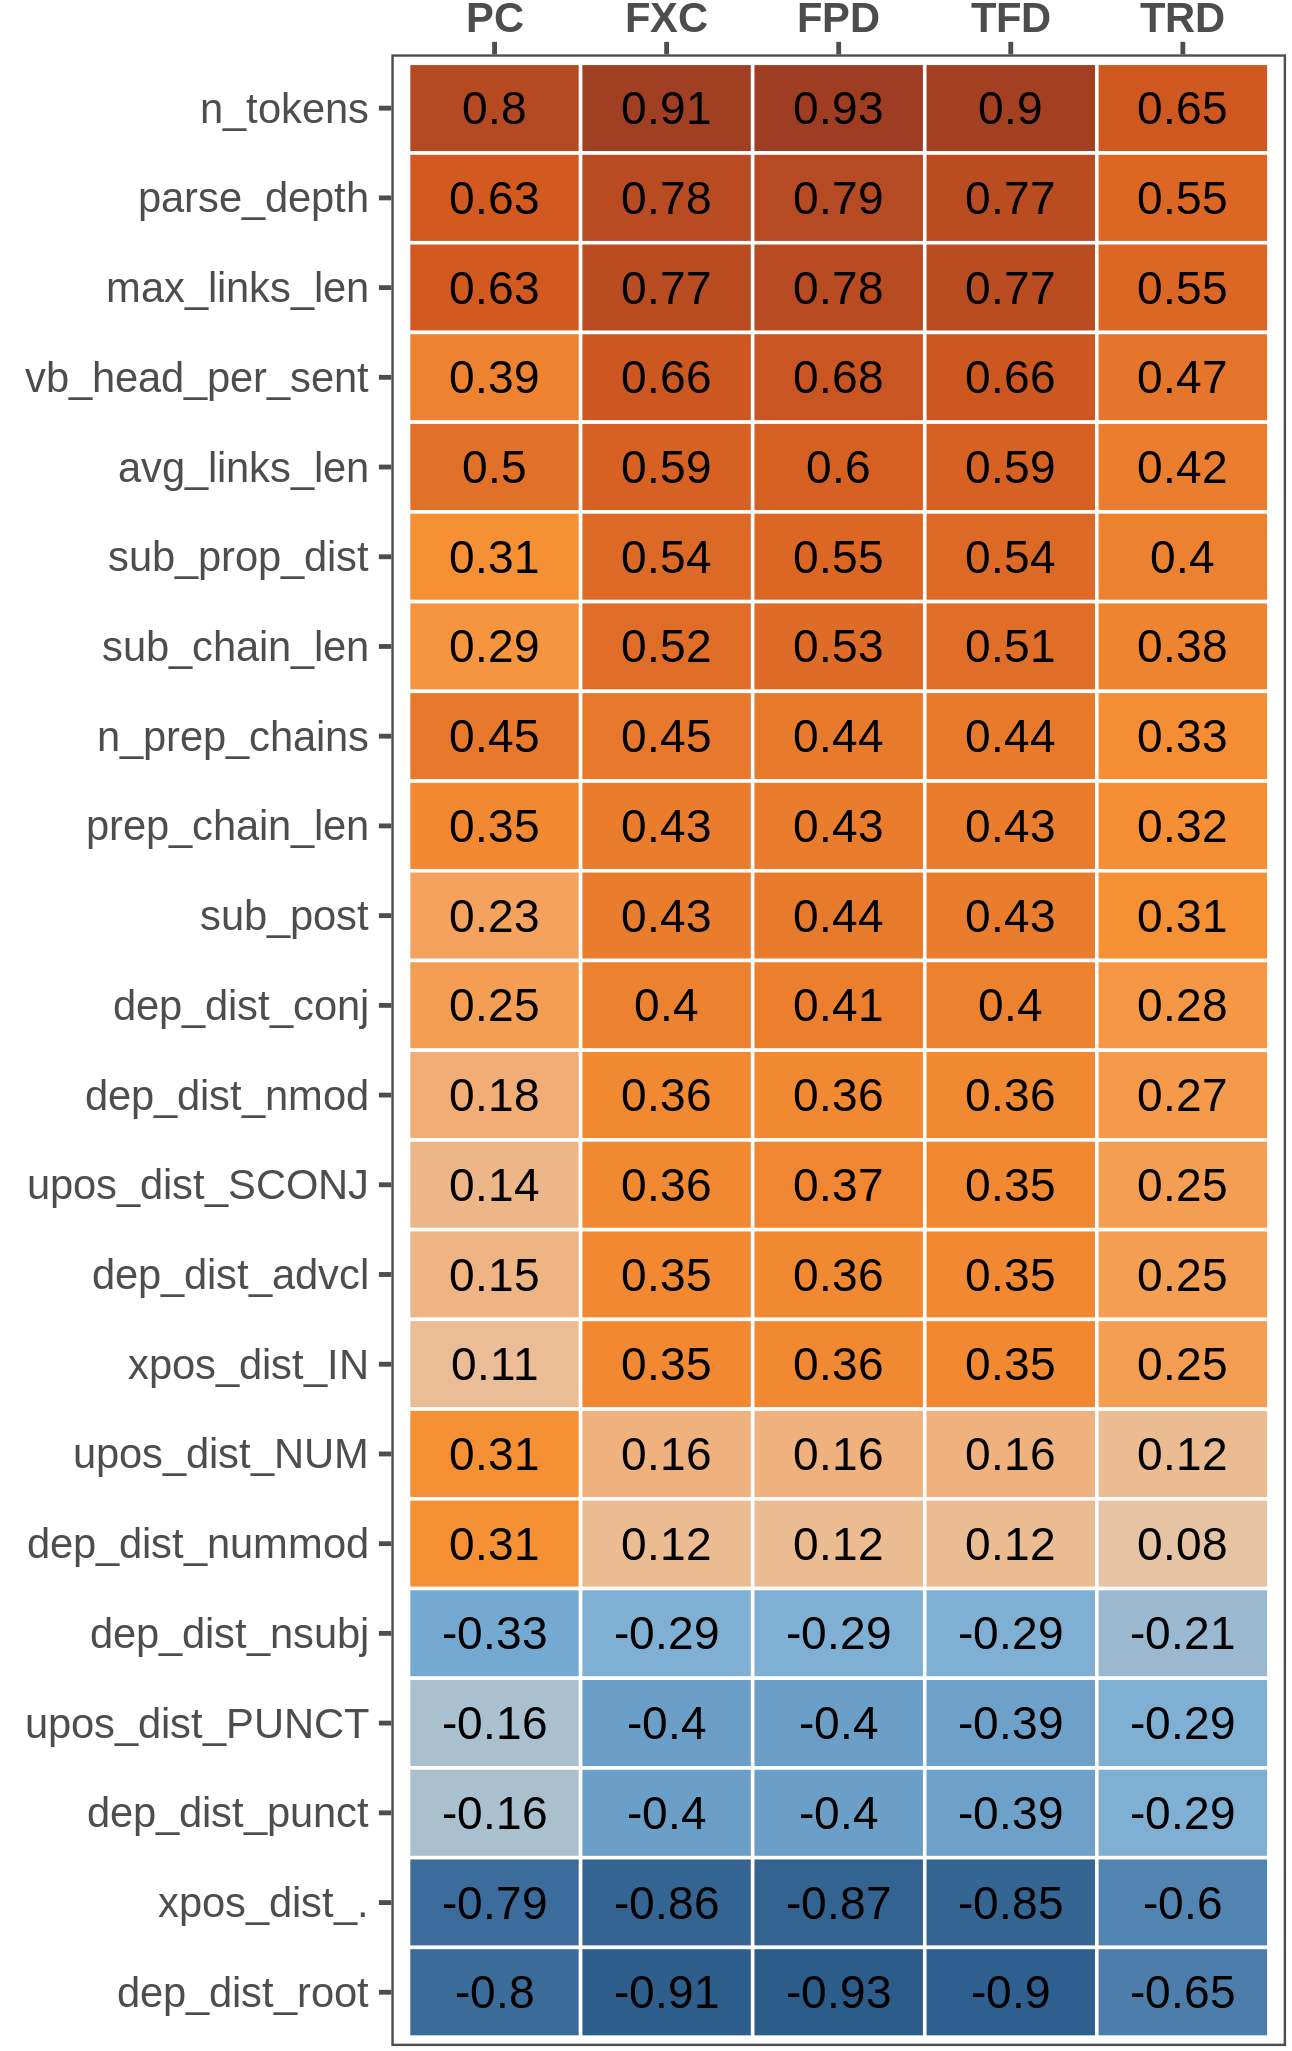
\includegraphics[width=0.5\linewidth]{figures/3_feat_heatmap} 

}

\caption{Ranking of the most correlated linguistic features for selected metrics. All of Spearman's correlation coefficients have \(p<0.001\).}\label{fig:feat-heatmap}
\end{figure}

The correlation scores analysis highlights how features showing a significant correlation with eye-tracking metrics are twice as many as those correlating with PC scores and generally tend to have higher coefficients, except for the total regression duration (TRD) metric. Nevertheless, the most correlated features are the same across all metrics. Figure \ref{fig:feat-heatmap} reports correlation scores for features showing a strong connection (\(|\rho|>0.3\)) with at least one of the evaluated metrics. As expected, sentence length (\emph{n\_tokens}) and other related features capturing structural complexity aspects occupy the top positions in the ranking. Among those, we can note the length of dependency links (\emph{max\_links\_len, avg\_links\_len}) and the depth of the whole parse tree or selected sub-trees, i.e.~nominal chains headed by a preposition (\emph{parse\_depth, n\_prep\_chains}).
Similarly, the distribution of subordinate clauses (\emph{sub\_prop\_dist, sub\_post}) is positively correlated with all metrics but with a more substantial effect for eye-tracking ones, especially in the presence of longer embedded chains (\emph{sub\_chain\_len}).
Interestingly, the presence of numbers (\emph{upos\_NUM, dep\_nummod}) affects only the offline perception of complexity, while it is never strongly correlated with all eye-tracking metrics. This finding is expected since numbers are very short tokens and, like other functional POS, were never found to be strongly correlated with online reading in our results. Conversely, numerical information has been identified as a factor hampering sentence readability and understanding \autocite{rello-etal-2013-one}.

\hypertarget{subsubchap:ex1-analysis-bins}{%
\subsection{Linguistic Phenomena in Length-controlled Bins}\label{subsubchap:ex1-analysis-bins}}

Unsurprisingly, sentence length is the most correlated predictor for all complexity metrics. Since many linguistic features highlighted in our analysis are strongly related to sentence length, we tested whether they maintain a relevant influence when this parameter is controlled. To this end, Spearman's correlation was computed between features and complexity tasks, but this time considering bins of sentences having approximately the same length. Specifically, we split each corpus into six bins of sentences with 10, 15, 20, 25, 30, and 35 tokens, respectively, with a range of ±1 tokens per bin to select a reasonable number of sentences for our analysis. Resulting subsets have a relatively constant size for the PC corpus, which was constructed ad-hoc to have such uniform length distribution, but have a sharply decreasing size for the eye-tracking corpus (see Table \ref{tab:ex1-stats}, bott. While deemed appropriate in the context of this correlation analysis, the disparity in bin sizes may play a significant role in hampering the performances of models trained on binned linguistic complexity data. This perspective is discussed in Section \ref{subchap:ex1-modeling}.



\begin{figure}

{\centering 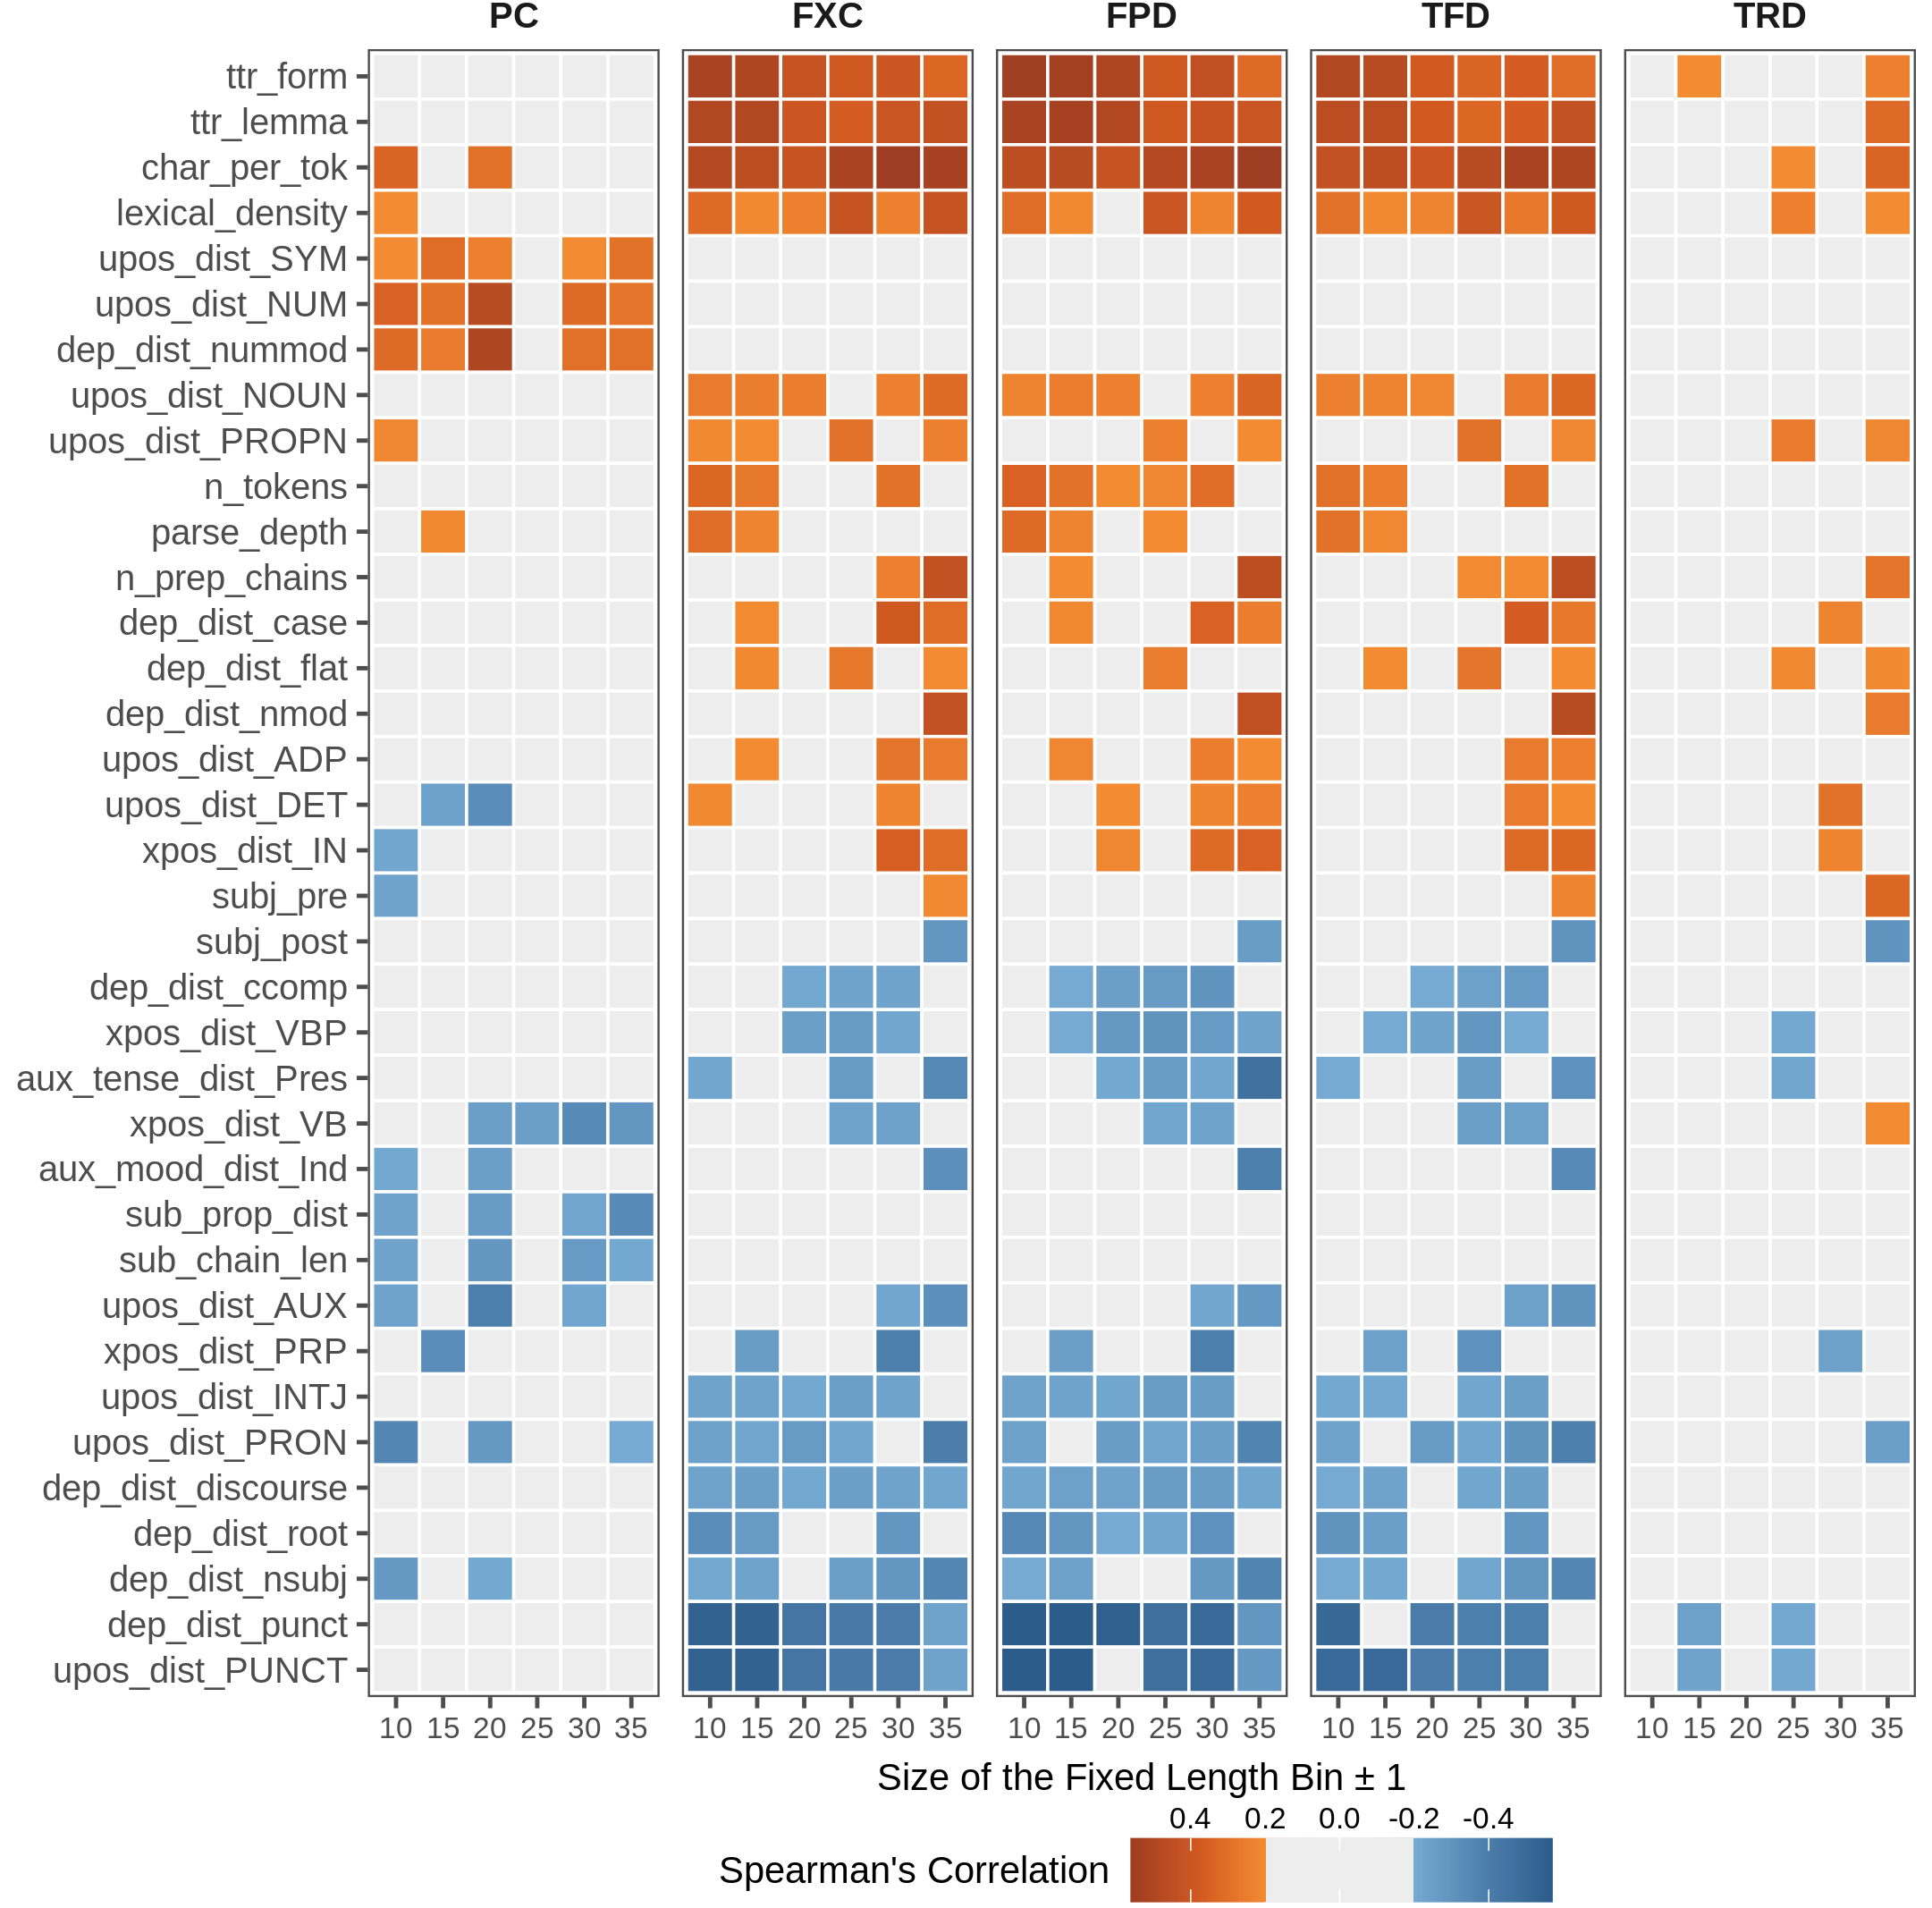
\includegraphics[width=0.95\linewidth]{figures/3_feat_bin_heatmap} 

}

\caption{Rankings of the most correlated linguistic features for metrics within length-binned subsets of the two corpora. Squares show the correlation between features (left axis) and a complexity metric (top) at a specific bin of length (bottom). Coefficients \(\geq\) 0.2 or \(\leq\) -0.2 are highlighted, and have \(p<0.001\).}\label{fig:feat-bin-heatmap}
\end{figure}

Figure \ref{fig:feat-bin-heatmap} reports the new rankings of the most correlated linguistic features within each bin across complexity metrics (\(|\rho| > 0.2\)). Again, we observe that features showing a significant correlation with complexity scores are fewer for PC bins than for eye-tracking ones. This fact depends on controlling for sentence length and the small size of bins for the whole dataset. As in the coarse-grained analysis, TRD is the eye-tracking metric less correlated to linguistic features, while the other three (FXC, FPD, TFD) show a homogeneous behavior across bins. For the latter, vocabulary-related features (token-type ratio, average word length, lexical density) are always positive and top-ranked in all bins, especially when considering shorter sentences (i.e.~from 10 to 20 tokens). For PC, this is true only for some of them (word length and lexical density). On another note, features encoding numerical information are still highly correlated with the offline perception of complexity in almost all bins.

Interestingly, features modeling subordination phenomena extracted from fixed-length sentences exhibit a reverse trend than when extracted from the whole corpus, i.e.~they are negatively correlated with judgments. If, on the one hand, an increase in the presence of subordination for longer sentences (possibly making sentences more convoluted) was expected, on the other hand, when the length is controlled, findings suggest that subordinate structures are not necessarily perceived as a symptom of sentence complexity.

The analysis also highlights how linguistic features relevant to online and offline complexity are different when controlling for sentence length. This aspect, in particular, was not evident from the previous coarse-grained analysis. Despite blocking sentence length, gaze measures are still significantly connected to length-related phenomena (high correlation with \emph{n\_tokens} at various length bins). This observation can be possibly due to the ±1 margin applied for sentence selection and the high sensitivity of behavioral metrics to small input changes.

\hypertarget{subchap:ex1-modeling}{%
\section{Modeling Online and Offline Linguistic Complexity}\label{subchap:ex1-modeling}}

Given the high correlations reported above, the next step involves quantifying the importance of explicit linguistic features from a modeling standpoint. Table \ref{tab:ex1-results} presents the RMSE and \(R^2\) scores of predictions made by baselines and models for the selected complexity metrics. Performances are tested with a 5-fold cross-validation regression with a fixed random seed on each metric. Our baselines use average metric scores of all training sentences (\emph{Avg. score}) and average scores of sentences binned by their length, expressed in number of tokens, as predictions (\emph{Bin average}). The two linear SVM models leverage explicit linguistic features, using respectively only the \emph{n\_tokens} feature (\emph{SVM length}) and the whole set of linguistic features presented above (\emph{SVM feats}). Besides those, the performances of a state-of-the-art Transformer neural language model relying entirely on contextual word embeddings are equally tested. \emph{ALBERT} (\textcite{lan-etal-2020-albert}; see Section \ref{subchap:nlm}) as a lightweight yet effective alternative to BERT \autocite{devlin-etal-2019-bert} for obtaining contextual word representations, using its last-layer \texttt{{[}CLS{]}} sentence embedding as input for a linear regressor during fine-tuning and testing. We selected the last layer representations, despite strong evidence on the importance of intermediate representation in encoding language properties, because we aim to investigate how superficial layers encode complexity-related competence. Given the availability of parallel eye-tracking annotations, we train ALBERT using multitask learning with hard parameter sharing \autocite{caruana-1997-multitask} on gaze metrics.\footnote{Training procedure and parameters are thoroughly described in Appendix \ref{app:params}.}

\begin{table}

\caption{\label{tab:ex1-results}Average Root-Mean-Square Error ($\sqrt{E^2}$) and $R^2$ score values for sentence-level complexity predictions using 5-fold cross-validation. Lower $\sqrt{E^2}$ and higher $R^2$ are better.}
\centering
\fontsize{11}{13}\selectfont
\begin{tabular}[t]{>{\raggedright\arraybackslash}p{10em}cccccccccc}
\toprule
\multicolumn{1}{c}{\textbf{ }} & \multicolumn{2}{c}{\textbf{PC}} & \multicolumn{2}{c}{\textbf{FXC}} & \multicolumn{2}{c}{\textbf{FPD}} & \multicolumn{2}{c}{\textbf{TFD}} & \multicolumn{2}{c}{\textbf{TRD}} \\
\cmidrule(l{3pt}r{3pt}){2-3} \cmidrule(l{3pt}r{3pt}){4-5} \cmidrule(l{3pt}r{3pt}){6-7} \cmidrule(l{3pt}r{3pt}){8-9} \cmidrule(l{3pt}r{3pt}){10-11}
 & $\sqrt{E^2}$ & $R^2$ & $\sqrt{E^2}$ & $R^2$ & $\sqrt{E^2}$ & $R^2$ & $\sqrt{E^2}$ & $R^2$ & $\sqrt{E^2}$ & $R^2$\\
\midrule
\addlinespace[0.3em]
\multicolumn{11}{l}{\textbf{Statistical baselines}}\\
\hspace{1em}Avg. score & 0.87 & 0 & 6.17 & 0.06 & 1078 & 0.06 & 1297 & 0.06 & 540 & 0.03\\
\hspace{1em}Bin average & 0.53 & 0.62 & 2.36 & 0.86 & 374 & 0.89 & 532 & 0.85 & 403 & 0.45\\
\hline
\addlinespace[0.3em]
\multicolumn{11}{l}{\textbf{Explicit features}}\\
\hspace{1em}SVM length & 0.54 & 0.62 & 2.19 & 0.88 & 343 & 0.9 & 494 & 0.86 & 405 & 0.45\\
\hspace{1em}SVM feats & \textbf{0.44} & 0.74 & \textbf{1.77} & \textbf{0.92} & \textbf{287} & \textbf{0.93} & \textbf{435} & \textbf{0.92} & 400 & 0.46\\
\hline
\addlinespace[0.3em]
\multicolumn{11}{l}{\textbf{Learned representations}}\\
\hspace{1em}ALBERT & \textbf{0.44} & \textbf{0.75} & 1.98 & \textbf{0.92} & 302 & \textbf{0.93} & \textbf{435} & 0.9 & \textbf{382} & \textbf{0.49}\\
\bottomrule
\end{tabular}
\end{table}

From Table \ref{tab:ex1-results} it can be noted that:

\begin{itemize}
\item
  The length-binned average baseline is very effective in predicting complexity scores and gaze metrics, which is unsurprising given the extreme correlation between length and complexity metrics presented in Figure \ref{fig:feat-heatmap};
\item
  The \emph{SVM feats} model shows considerable improvements if compared to the length-only SVM model for all complexity metrics, highlighting how length alone accounts for much but not for the entirety of variance in complexity scores;
\item
  ALBERT performs on-par with the SVM feats model on all complexity metrics despite the small dimension of the fine-tuning corpora and the absence of explicit linguistic information.
\end{itemize}

A possible interpretation of ALBERT's strong performances is that the model implicitly develops competence related to phenomena encoded by linguistic features while training on online and offline complexity prediction. We explore this perspective in Section \ref{subchap:ex1-probing}.

\hypertarget{subsubchap:ex1-modeling-bins}{%
\subsection{Modeling Complexity in Length-controlled Bins}\label{subsubchap:ex1-modeling-bins}}



\begin{figure}

{\centering 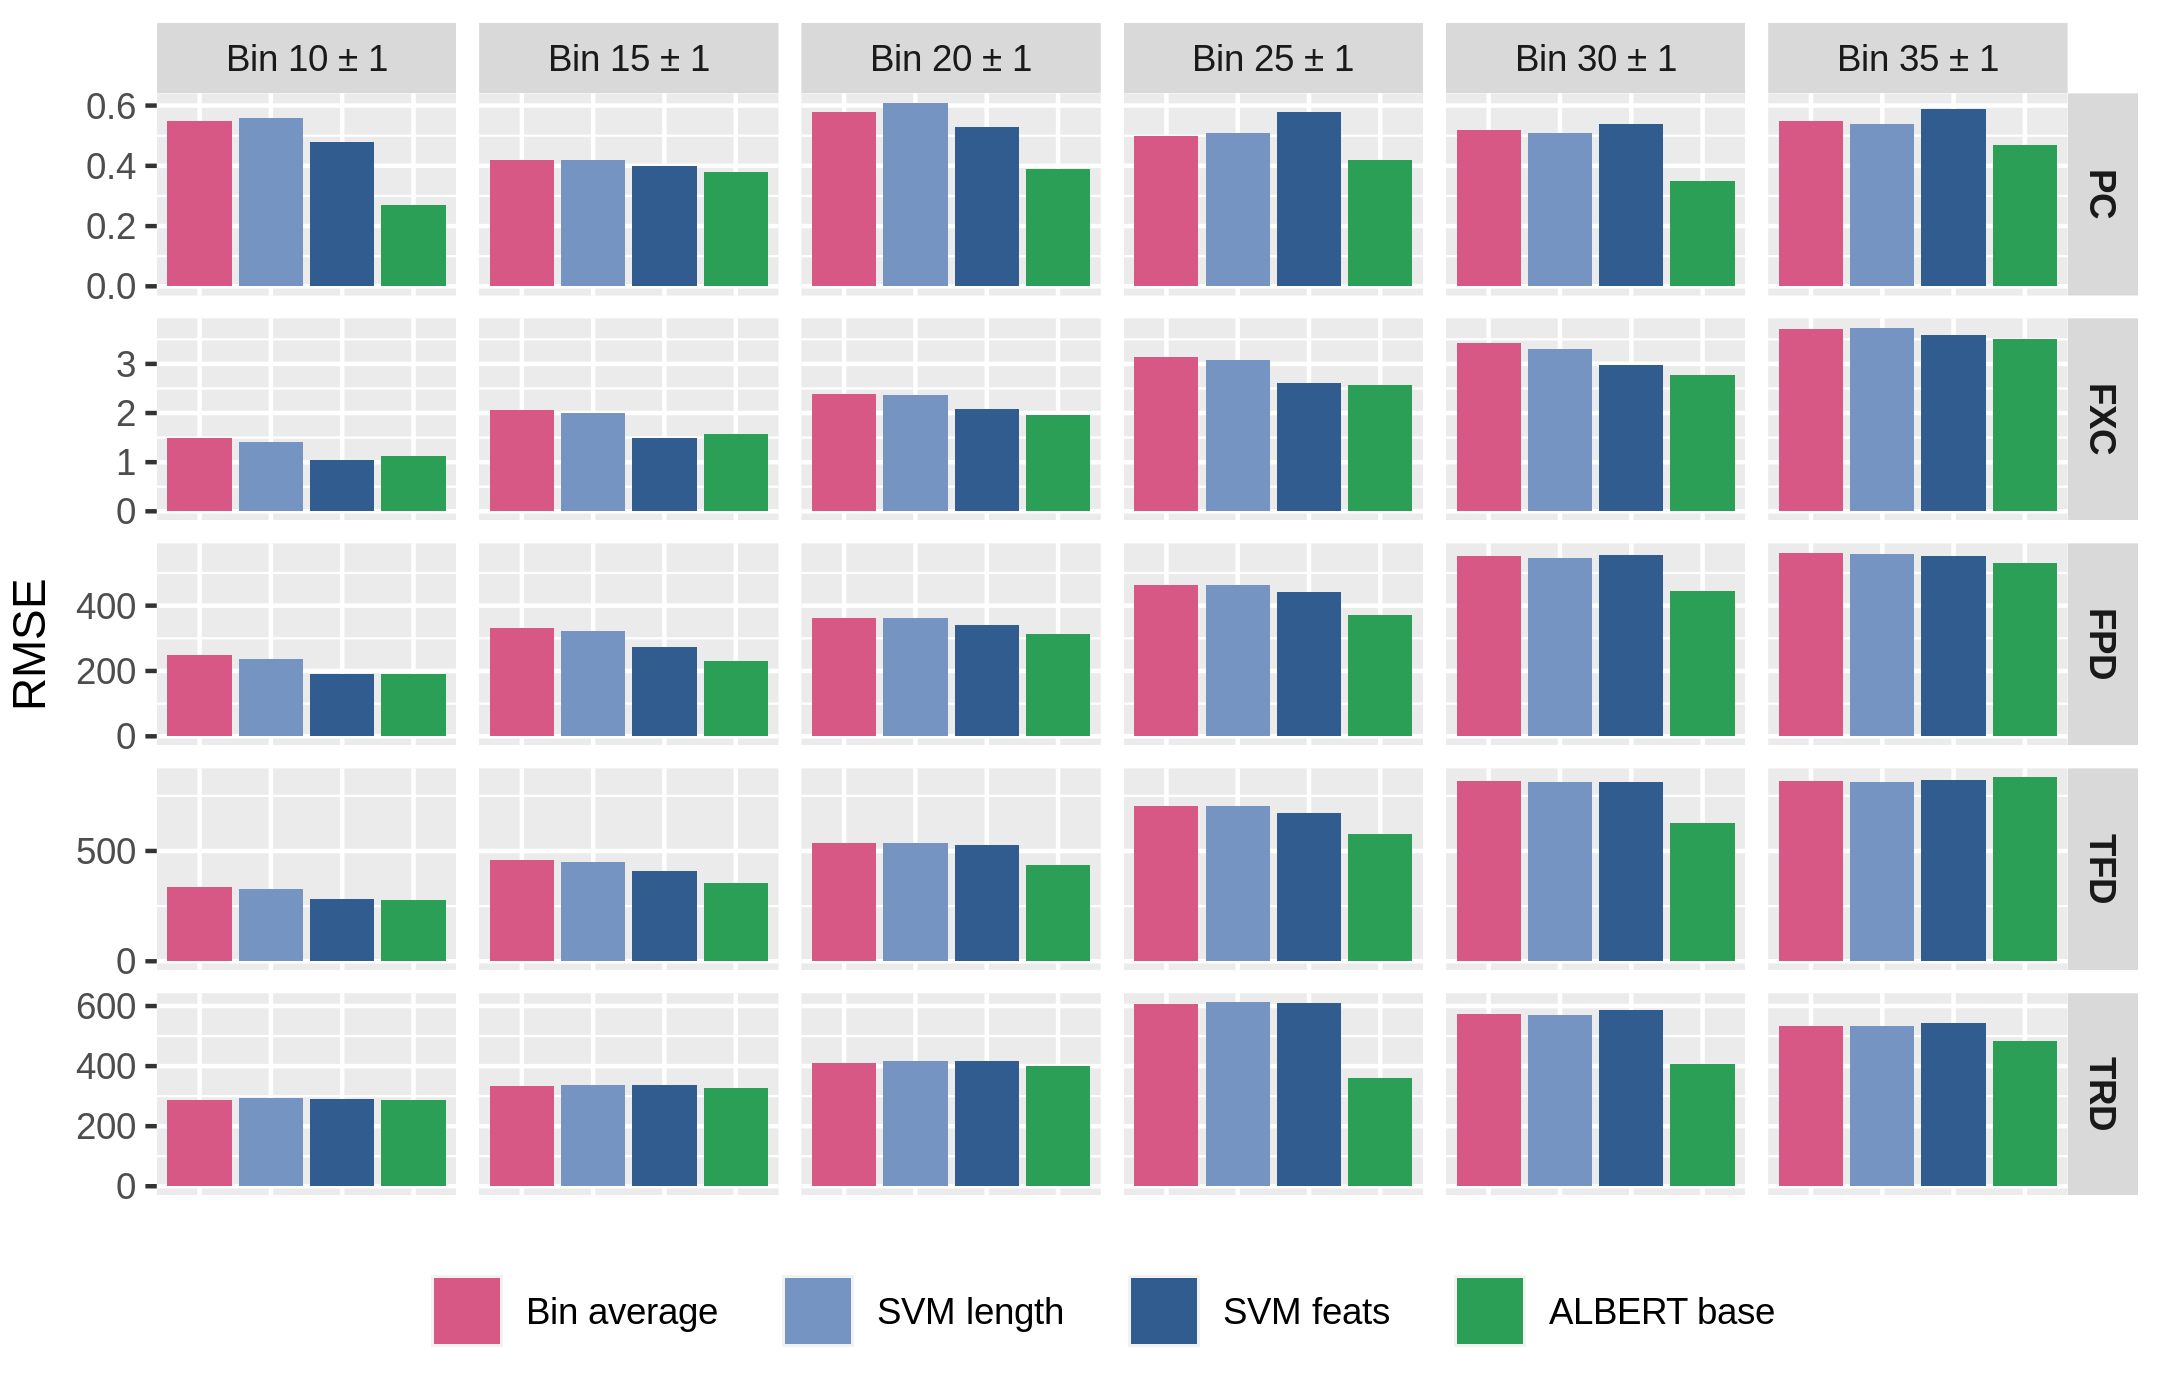
\includegraphics[width=1\linewidth]{figures/3_models_bin_scores} 

}

\caption{Average Root-Mean-Square Error (RMSE) scores for models in Table \ref{tab:ex1-results}, performing 5-fold cross-validation on the length-binned subsets used for Figure \ref{fig:feat-bin-heatmap}. Lower scores are better.}\label{fig:models-bin-scores}
\end{figure}

Similarly to the approach adopted in Section \ref{subsubchap:ex1-analysis-bins}, the performances of models are tested on length-binned data to verify their consistency in the context of length-controlled sequences. Figure \ref{fig:models-bin-scores} presents RMSE scores averaged with 5-fold cross-validation over the length-binned sentences subsets for all complexity metrics. It can be observed that ALBERT outperforms the SVM with linguistic features on nearly all bins and metrics, showing the largest gains on intermediate bins for PC and gaze durations (FPD, TFD, TRD). Interestingly, models' overall performances follow a length-dependent increasing trend for eye-tracking metrics, but not for PC. This behavior can be possibly explained in terms of the high sensibility to length previously highlighted for online metrics, as well as the broad variability in bin dimensions. It can also be observed how the SVM model based on explicit linguistic features (\emph{SVM feats}) performs poorly on larger bins for all tasks, sometimes being even worse than the bin-average baseline. While this behavior seems surprising given the positive influence of features highlighted in Table \ref{tab:ex1-results}, this phenomenon can be attributed to the small dimension of longer bins, which negatively impacts the generalization capabilities of the regressor. The relatively better scores achieved by ALBERT in those, instead, support the effectiveness of information stored in pretrained language representations when a limited number of examples are available.

\hypertarget{subchap:ex1-probing}{%
\section{Probing Linguistic Phenomena in ALBERT Representations}\label{subchap:ex1-probing}}

As shown in the previous section, ALBERT performances in complexity predictions are comparable to those of an SVM relying on explicit linguistic features and even better than those when controlling for length. The \emph{probing task} interpretability paradigm (Section \ref{subsubchap:probe}) is adopted to investigate if ALBERT encodes the linguistic knowledge that we identified as strongly correlated with online and perceived sentence complexity during training and prediction. In particular, the aim of this investigation is two-fold:

\begin{itemize}
\item
  Probing ALBERT's innate competence in relation to the broad spectrum of linguistic features described in Appendix \ref{app:ling-feats}; and
\item
  Verifying whether, and in which respect, this competence is affected by a fine-tuning process on the complexity assessment metrics.
\end{itemize}

Three UD English treebanks spanning different textual genres -- \textbf{EWT, GUM, and ParTUT} respectively by \textcite{silveira-etal-2014-gold}, \textcite{zeldes-2017-gum}, and \textcite{sanguinetti-etal-2015-partut} -- were aggregated, obtaining a final corpus of 18,079 sentences with gold linguistic information which was used to conduct probing experiments. The Profiling-UD tool was again leveraged to extract \(n\) sentence-level linguistic features \(\mathcal{Z}=z_1, \dots, z_n\) from gold linguistic annotations. Representations \(A(x)\) were generated for all corpus sentences using the last-layer \texttt{{[}CLS{]}} embedding of a pretrained ALBERT base model without additional fine-tuning, and \(n\) single-layer perceptron regressors \(g_i: A(x) \rightarrow z_i\) are trained to map representations \(A(x)\) to each linguistic feature \(z_i\). Finally, the error and \(R^2\) scores of each \(g_i\) were evaluated as proxies for the quality of representations \(A(x)\) in encoding their respective linguistic feature \(z_i\). The same evaluation is repeated for ALBERTs fine-tuned respectively on perceived complexity labels (PC) and on all eye-tracking labels with multitask learning (ET), averaging scores with 5-fold cross-validation. A selected subset of results is shown on the left side of Table \ref{tab:probes}.

\begin{table}

\caption{\label{tab:probes}Root MSE ($\sqrt{E^2}$) and $R^2$ scores for diagnostic regressors trained on ALBERT representations, respectively, without fine-tuning (Base), with PC and eye-tracking (ET) fine-tuning on all data (left) and on the $10 \pm 1$ length-binned subset (right). \textbf{Bold} values highlight relevant increases in $R^2$ from Base.}
\centering
\fontsize{11}{13}\selectfont
\begin{tabular}[t]{lccccc>{}c|cccc}
\toprule
\multicolumn{1}{c}{\textbf{ }} & \multicolumn{2}{c}{\textbf{Base}} & \multicolumn{2}{c}{\textbf{PC}} & \multicolumn{2}{c}{\textbf{ET}} & \multicolumn{2}{c}{\textbf{PC10±1}} & \multicolumn{2}{c}{\textbf{ET10±1}} \\
\cmidrule(l{3pt}r{3pt}){2-3} \cmidrule(l{3pt}r{3pt}){4-5} \cmidrule(l{3pt}r{3pt}){6-7} \cmidrule(l{3pt}r{3pt}){8-9} \cmidrule(l{3pt}r{3pt}){10-11}
 & $\sqrt{E^2}$ & $R^2$ & $\sqrt{E^2}$ & $R^2$ & $\sqrt{E^2}$ & $R^2$ & $\sqrt{E^2}$ & $R^2$ & $\sqrt{E^2}$ & $R^2$\\
\midrule
n\_tokens & 8.19 & 0.26 & 4.66 & \textbf{0.76} & 2.87 & \textbf{0.91} & 8.66 & 0.18 & 6.71 & \textbf{0.51}\\
parse\_depth & 1.47 & 0.18 & 1.18 & \textbf{0.48} & 1.04 & \textbf{0.6} & 1.50 & 0.16 & 1.22 & \textbf{0.43}\\
vb\_head\_per\_sent & 1.38 & 0.15 & 1.26 & \textbf{0.3} & 1.14 & \textbf{0.42} & 1.44 & 0.09 & 1.30 & \textbf{0.25}\\
xpos\_dist\_. & 0.05 & 0.13 & 0.04 & \textbf{0.41} & 0.04 & \textbf{0.42} & 0.04 & 0.18 & 0.04 & \textbf{0.38}\\
avg\_links\_len & 0.58 & 0.12 & 0.53 & \textbf{0.29} & 0.52 & \textbf{0.31} & 0.59 & 0.1 & 0.56 & \textbf{0.2}\\
max\_links\_len & 5.20 & 0.12 & 4.08 & \textbf{0.46} & 3.75 & \textbf{0.54} & 5.24 & 0.11 & 4.73 & \textbf{0.28}\\
n\_prep\_chains & 0.74 & 0.11 & 0.67 & \textbf{0.26} & 0.66 & \textbf{0.29} & 0.72 & 0.14 & 0.69 & \textbf{0.21}\\
sub\_prop\_dist & 0.35 & 0.09 & 0.33 & 0.13 & 0.31 & \textbf{0.22} & 0.34 & 0.05 & 0.32 & 0.15\\
upos\_dist\_PRON & 0.08 & 0.09 & 0.08 & 0.14 & 0.08 & 0.07 & 0.07 & \textbf{0.23} & 0.08 & 0.15\\
pos\_dist\_NUM & 0.05 & 0.08 & 0.05 & 0.06 & 0.05 & 0.02 & 0.05 & \textbf{0.16} & 0.05 & 0.06\\
dep\_dist\_nsubj & 0.06 & 0.08 & 0.06 & 0.1 & 0.06 & 0.05 & 0.05 & \textbf{0.17} & 0.06 & 0.11\\
char\_per\_tok & 0.89 & 0.07 & 0.87 & 0.12 & 0.90 & 0.05 & 0.82 & \textbf{0.22} & 0.86 & 0.14\\
prep\_chain\_len & 0.60 & 0.07 & 0.57 & \textbf{0.17} & 0.56 & \textbf{0.19} & 0.59 & 0.12 & 0.56 & \textbf{0.18}\\
sub\_chain\_len & 0.70 & 0.07 & 0.67 & \textbf{0.15} & 0.62 & \textbf{0.26} & 0.71 & 0.04 & 0.66 & \textbf{0.16}\\
dep\_dist\_punct & 0.07 & 0.06 & 0.07 & 0.06 & 0.07 & \textbf{0.14} & 0.07 & 0.06 & 0.07 & \textbf{0.14}\\
dep\_dist\_nmod & 0.05 & 0.06 & 0.05 & 0.07 & 0.05 & 0.06 & 0.05 & 0.09 & 0.05 & 0.09\\
sub\_post & 0.44 & 0.05 & 0.46 & 0.12 & 0.44 & \textbf{0.18} & 0.47 & 0.05 & 0.45 & \textbf{0.14}\\
dep\_dist\_case & 0.07 & 0.05 & 0.06 & 0.06 & 0.07 & 0.08 & 0.07 & 0.07 & 0.07 & 0.1\\
lexical\_density & 0.14 & 0.05 & 0.13 & 0.03 & 0.13 & 0.03 & 0.13 & \textbf{0.13} & 0.13 & \textbf{0.13}\\
dep\_dist\_compound & 0.06 & 0.04 & 0.06 & 0.05 & 0.06 & 0.03 & 0.06 & 0.1 & 0.06 & 0.07\\
dep\_dist\_conj & 0.04 & 0.03 & 0.04 & 0.04 & 0.04 & 0.04 & 0.05 & 0.02 & 0.04 & 0.03\\
ttr\_form & 0.08 & 0.03 & 0.08 & 0.05 & 0.08 & 0.05 & 0.08 & 0.05 & 0.08 & 0.05\\
dep\_dist\_det & 0.06 & 0.03 & 0.06 & 0.02 & 0.06 & 0.04 & 0.06 & 0.03 & 0.06 & 0.03\\
dep\_dist\_aux & 0.04 & 0.02 & 0.04 & 0.01 & 0.04 & 0.01 & 0.04 & 0.06 & 0.04 & 0.04\\
pos\_dist\_VBN & 0.03 & 0.01 & 0.03 & 0 & 0.03 & 0 & 0.03 & 0.01 & 0.03 & 0\\
xpos\_dist\_VBZ & 0.04 & 0.01 & 0.04 & 0.01 & 0.04 & 0.02 & 0.04 & 0.02 & 0.04 & 0.02\\
ttr\_lemma & 0.09 & 0.01 & 0.09 & 0.06 & 0.09 & 0.06 & 0.09 & 0.04 & 0.09 & 0.03\\
\bottomrule
\end{tabular}
\end{table}

As it can be observed, ALBERT's last-layer sentence representations have relatively low knowledge of complexity-related probes, but their performances highly increase after fine-tuning. Specifically, a noticeable improvement was obtained on features that were already better encoded in base pretrained representation, i.e.~sentence length and related, suggesting that fine-tuning possibly accentuates only properties already well-known by the model, regardless of the target task. To verify that this isn't the case, the same probing tests were repeated on ALBERT models fine-tuned on the smallest length-binned subset (i.e. \(10\pm1\) tokens) presented in previous sections. The right side of Table \ref{tab:probes} presents the resulting scores. From the length-binned correlation analysis of Section \ref{fig:feat-bin-heatmap}, PC scores were observed to be mostly uncorrelated with length phenomena, while ET scores remain significantly affected despite our controlling of sequence size. This observation also holds for length-binned probing task results, where the PC model seems to neglect length-related properties in favor of task-specific ones that were also highlighted in our fine-grained correlation analysis (e.g.~word length, numbers, explicit subjects). The ET-trained model follows the same behavior, retaining strong but lower performances for length-related features.

In conclusion, although higher probing task performances after fine-tuning are not direct proof that the neural language model exploits newly-acquired morpho-syntactic and syntactic information, results suggest that training on tasks strongly connected with underlying linguistic structures triggers a change in model representations resulting in a better encoding of related linguistic properties.

\hypertarget{subchap:ex1-summary}{%
\section{Summary}\label{subchap:ex1-summary}}

In this chapter, the connection between eye-tracking metrics and the offline perception of sentence complexity was investigated from an experimental standpoint. An in-depth correlation analysis was performed between complexity scores and sentence linguistic properties at different granularity levels, highlighting the strong relationship between metrics and length-affine properties and revealing different behaviors when controlling for sentence length. Models using explicit linguistic features and unsupervised word embeddings were evaluated on complexity prediction, showing comparable performances across metrics. Finally, the encoding of linguistic properties in a neural language model's contextual representations was tested with probing tasks. This approach highlighted the natural emergence of task-related linguistic properties within the model's representations after the fine-tuning process. Thus, it can be conjectured that a relation subsists between the model's linguistic abilities during the training procedure and its downstream performances on morphosyntactically-related tasks and that linguistic probes may provide a reasonable estimate of the task-oriented quality of representations.

\hypertarget{chap:ex2}{%
\chapter{\texorpdfstring{\textbf{Representational Similarity in Models of Complexity}}{Representational Similarity in Models of Complexity}}\label{chap:ex2}}

\minitoc 

\chaptermark{Representational Similarity in Models of Complexity}

\begin{quote}
The experiments of this chapter aim to shed light on how the linguistic knowledge encoded in the contextual representations of complexity-trained neural language models varies across layers of abstraction and fine-tuning tasks. Two similarity approaches, Representational Similarity Analysis (RSA) and Projection-Weighted Canonical Correlation Analysis (PWCCA) are used to evaluate the relation subsisting between representations spanning different models and different layers of the same model. The outcomes are finally compared against a set of assumptions aimed at determining a model's generalization capabilities across language phenomena. Results provide empirical evidence about the inability of state-of-the-art language modeling approaches to effectively represent an abstract hierarchy of linguistic complexity phenomena.
\end{quote}

Chapter \ref{chap:ex1} highlighted how the relation between online and offline complexity perspectives and linguistic phenomena diverge when considering same-length sentences and how those properties of language are adequately captured by a neural language model fine-tuned on complexity metrics. This chapter adopts a complementary perspective on the model-driven study of complexity. Instead of connecting learned representations to the input's structural properties, it explores how those representations change when the same model is exposed to different training objectives using similarity measures. This approach is used to gain insights on the underlying similarities across complexity metrics, using representations as proxies for the knowledge needed to correctly model various complexity phenomena under a minimal set of assumptions.

The same ALBERT \autocite{lan-etal-2020-albert} model introduced in Section \ref{subchap:nlm} and used for the last section's probing task experiments is leveraged for this chapter's experiments.\footnote{The \texttt{albert-base-v2} checkpoint from 🤗 \texttt{transformers} \autocite{wolf-etal-2020-huggingface} is used.} The model is first taken as-is in its pre-trained version without fine-tuning (referred to as \textbf{Base}). Then, three instances of it are fine-tuned respectively on \textbf{Automatic Readability Assessment} (RA, Section \ref{subsubchap:readability}), \textbf{Perceived Complexity Prediction} (PC, Section \ref{subsubchap:pc}) and \textbf{Eye-tracking Metrics Prediction} (ET, Section \ref{subsubchap:eye-tracking}) until convergence. The four models are evaluated in two settings: first, by comparing the similarity of same-layer representation across models (\emph{inter-model similarity}), and then comparing the similarity across different layers of the same model (\emph{intra-model similarity}). For each setting, two similarity metrics are used: Representational Similarity Analysis (RSA, Section \ref{subsubchap:rsa}) and Projection-Weighted Canonical Correlation Analysis (PWCCA, Section \ref{subsubchap:pwcca}). RSA and PWCCA were selected since they provide different perspectives over the similarity of representations: if, on the one hand, RSA naively evaluates the similarity across input representations through correlation, PWCCA factors in the importance of sparsity patterns that characterize overparametrized neural networks using a projection operation. Both token and sentence-level representations are evaluated to obtain a fine-grained overview of representational similarity.

The models trained on perceived complexity and eye-tracking metrics are again the main subjects of this study, given the logical and empirical relation subsisting between the two complexity perspectives highlighted in previous chapters. The additional use of Base and readability-trained models allows us to verify whether ALBERT representations satisfy a minimal set of assumptions deemed necessary and sufficient for modeling an abstraction hierarchy of linguistic complexity phenomena in an interpretable fashion. Results produced by representational similarity experiments diverge significantly from the initial hypothesis, suggesting the prominence of surface structures and task setups over underlying general knowledge about the nature of the modeled phenomena in shaping representations during the training process.

\paragraph{Contributions} While multiple works aimed at inspecting NLM representations by mean of similarity approaches already exist, this is the first work to the best of my knowledge that does so with the explicit purpose of evaluating the impact of linguistic complexity training. This work:

\begin{itemize}
\item
  Highlights similarity and differences in the representations of models trained on different complexity-related tasks to understand how neural network parameters capture different perspectives over linguistic complexity after the training process;
\item
  Presents similarity and differences in the representations found at different layers of the same model to understand how knowledge is distributed hierarchically at various abstraction levels after training;
\item
  Provide evidence about the inability of state-of-the-art NLP approaches to learning to effectively represent an abstract hierarchy of linguistic complexity phenomena in an unsupervised manner, relying solely on complexity-related annotations.\footnote{Code available at \url{https://github.com/gsarti/interpreting-complexity}}
\end{itemize}

\hypertarget{knowledge-driven-requirements-for-learning-models}{%
\section{Knowledge-driven Requirements for Learning Models}\label{knowledge-driven-requirements-for-learning-models}}

At the beginning of Chapter \ref{chap:models} two prerequisites to any model-driven study were defined: that available annotated corpora should be informative about the underlying phenomena we are trying to model, and that sufficiently elaborate models should be able to represent knowledge to solve phenomena-related tasks after being trained on those corpora effectively. This section formalizes the two assumptions and builds upon them to define a set of fundamental requirements that should be satisfied by models capable of generalizing over unseen linguistic structures after undergoing a learning process. Let:

\begin{itemize}
\item
  \(\mathcal{C}^\phi_\alpha = \Big [ (x_1,\alpha_1)\dots(x_m,\alpha_m)\Big]\) be an annotated corpus containing some knowledge relative to an abstract phenomenon of interest \(\phi\) encoded in its annotations \(\alpha\). \(x\) can represent any \(i\)-th linguistic structure or substructure (sentence, word, morpheme). This notation can be generalized to settings where annotations are not explicitly defined (e.g.~in the context of language modeling, next structure \(x_i+1\) acts as an annotation for \(x_i\)) or when multiple annotations are present (e.g.~if \(\mathcal{C}\) has two sets of annotations \(\alpha, \beta\) modeling the same phenomenon \(\mathcal{K}\) is equivalent to two corpora \(\mathcal{C}^\phi_\alpha, \mathcal{C}^\phi_\beta\) with shared \(x\)'s).
\item
  \(M\) be a model that, after being trained on \(\mathcal{C}^{\phi}_\alpha\), learns representations (i.e.~parameters) that allow him to map correctly linguistic structures to annotations
\item
  \(\mathcal{K}^\phi\) be a set containing all empirical knowledge that is specifically relevant to phenomenon \(\phi\). \(\mathcal{K}^\phi_\alpha\) represents all knowledge relative to \(\phi\) contained in a corpus \(\mathcal{C}^\phi_\alpha\). Concretely, given a corpus \(\mathcal{C}^\phi_\alpha\), we can logically infer from it some estimate knowledge \(\tilde{\mathcal{K}}^\phi_\alpha\) such that \(\tilde{\mathcal{K}}^\phi_\alpha \simeq \mathcal{K}^\phi_\alpha \subset \mathcal{K}^\phi\).
\item
  \(\varsigma_{\alpha, \beta}^{\phi}(x)\) be an idealized similarity function reflecting the similarity between two sets of representations in performance-driven terms relative to phenomenon \(\phi\), i.e.~measuring their invariance in relation to all knowledge sets \(\mathcal{K}^\varphi\), with \(\phi \neq \varphi\) that are irrelevant to phenomenon \(\phi\).
\end{itemize}

For example, taking linguistic complexity as \(\phi\), and the GECO corpus as \(\mathcal{C}^\phi_\alpha\) (with \(\alpha\) being e.g.~the total fixation duration annotations), we may have \(\tilde{\mathcal{K}}^\phi_\alpha\) (i.e.~our inferred knowledge about linguistic complexity) contains the observation \(o =\) ``longer structures are more complex'' because longer words have longer total fixation durations on average. Note that the relation \(o \in \mathcal{K}^\phi_\alpha\) can only be hypothesized whenever a corpus with different annotations \(\mathcal{C}^\phi_\beta\) pertinent to the same phenomenon allows us to infer a \(\tilde{\mathcal{K}}^\phi_\beta\) such that \(o \in \tilde{\mathcal{K}}^\phi_\alpha \cap \tilde{\mathcal{K}}^\phi_\beta\) (e.g.~longer sentences are also deemed more complex on average in the perceived complexity corpus, so length is probably related to complexity in general).

Chapter \ref{chap:models} assumptions can now be summarized in a single statement:

\vspace{-12pt}

\paragraph{Assumption 4.1} (Learning-driven encodability) A learning process that trains a model \(M\) on a corpus \(\mathcal{C}^\phi_\alpha\) up to a reasonable accuracy is equivalent to an encoding function that maps \(\phi\)-relevant knowledge contained in \(\mathcal{C}^\phi_\alpha\) to \(M\)'s learned representations.

\vspace{10pt}

If Assumption 4.1 is verified, then annotations must be informative, and the model must be able to encode all knowledge present in the corpora relevant to the phenomena. On top of that foundational assumption, three further requirements that are sufficient and necessary for building interpretable learning models able to represent knowledge in a generalizable manner are defined:

\paragraph{Assumption 4.2} (Knowledge-similarity interrelation) Given two corpora \(\mathcal{C}^\phi_\alpha, \mathcal{C}^\phi_\beta\) providing different and possibly complementary knowledge about the same phenomenon \(\phi\) and representations \(R^{M}_{\alpha}, R^{M}_{\beta}\) learned by a model \(M\) trained respectively on the two corpora, the more those representations are similar in relation to \(\phi\), the more \(\phi\)-related shared knowledge is contained in the two corpora. When the two representations are perfectly \(\phi\)-similar, the two corpora share the same \(\phi\)-related knowledge.

\paragraph{Assumption 4.3} (Pertinence-based preponderance) The amount of knowledge \(\mathcal{K}^\phi_\alpha\) related to phenomenon \(\phi\) contained in a corpus \(\mathcal{C}^{\phi}_\alpha\) that explicitly encodes some knowledge about \(\phi\) is always larger than the amount of knowledge relative to \(\phi\) contained in any corpus \(\mathcal{C}^{\phi'}_\beta\) which explicitly covers a different phenomenon \(\phi'\) by means of its annotations \(\beta\).

\paragraph{Assumption 4.4} (Knowledge-similarity transitivity) Given three corpora \(\mathcal{C}^\phi_\alpha, \mathcal{C}^\phi_\beta, \mathcal{C}^\phi_\gamma\) providing different views over the same phenomenon \(\phi\) and representations \(R^{M}_{\alpha}, R^{M}_{\beta}, R^{M}_{\gamma}\) learned by a model \(M\) trained on each one of them respectively, if a pair of those representations has higher \(\phi\)-similarity than another, then the respective pair of corpora also have a larger amount of shared \(\phi\)-related knowledge and vice versa.

The experimental section of this chapter is aimed at testing whether those requirements are satisfied by ALBERT. Assumption 4.2 enables us to use representational similarity measures to evaluate our corpora's latent knowledge related to linguistic complexity. In particular, RSA and PWCCA will be used respectively as naive and more advanced approximations of \(\varsigma\) that evaluate representations' distance in the \(n\)-dimensional space across multiple linguistic structures.

The first step in this verification process involves comparing representations learned by ALBERT models trained on PC, ET, and RA against those of Base. Since the base model was exposed to a general MLM pre-training, without having access to any complexity-related annotation, it can be hypothesized that \emph{the three complexity-trained models had access to more complexity-related information during training} (Assumptions 4.1 and 4.3), \emph{and thus learned representations that are closer together in similarity terms than those of Base} (Assumption 4.2). The other perspective involves evaluating how different views related to the same phenomenon are captured. While perceived complexity annotations and gaze metrics are at the antipodes of the processing spectrum (see Figure \ref{fig:compass}), they should logically contain more complexity-related shared information than readability categories since they are both related to the reader's viewpoint, while RA captures the writer's perspective. If Assumption 4.4 is verified, then it can be hypothesized that \emph{ALBERT-PC and ALBERT-ET learned representations closer together in similarity terms than those of the ALBERT-RA model}.

Before moving to the experiments, two crucial aspects should be highlighted. First, corpus size was abstracted away from the verification process despite being commonly known to be an essential factor in shaping neural network training effectiveness. In particular, we should be aware that the size imbalance across available corpora can be a significant source of error in the evaluation process. Secondly, sentence-level training objectives are used for PC and RA tasks, while ALBERT-ET is trained on token-level annotations.\footnote{More details on this procedure are provided in Appendix \ref{app:et-modeling}.} If, on the one hand, this difference in training approaches can act as an additional confounder when evaluating requirements, from another perspective, it can provide us with some information relative to the generalization abilities of ALBERT beyond task setup.

\hypertarget{subchap:ex2-experiments}{%
\section{Experimentsl Evaluation}\label{subchap:ex2-experiments}}

This section describes the similarity experiments that have been carried out over model representations across multiple training setups. First, Section \ref{subsubchap:ex2-data} presents the data used to train ALBERT models and evaluate their representational similarity. Then, Section \ref{subsubchap:ex2-inter} focuses on validating the assumptions formulated at the beginning of this chapter by evaluating the intra-model similarity across all model pairs. Finally, Section \ref{subsubchap:ex2-intra} employs the same similarity approach in an intra-model setting, providing us with some evidence on how linguistic knowledge is encoded hierarchically across ALBERT layers during the training process.

\hypertarget{subsubchap:ex2-data}{%
\subsection{Data}\label{subsubchap:ex2-data}}

The experiments of this chapter leverage all corpora that were presented in Sections \ref{subsubchap:readability}, \ref{subsubchap:pc} and \ref{subsubchap:eye-tracking} for fine-tuning the three complexity models whose representations were compared against each other and the Base pre-trained ALBERT. Specifically:

\vspace{-12pt}

\paragraph{Readability Assessment} The OneStopEnglish corpus \autocite{vajjala-lucic-2018-onestopenglish} is leveraged by splitting each document into sentences and labeling those with the original reading level. A total of 7190 sentences equally distributed across the Elementary, Intermediate, and Advanced levels are used to fine-tune ALBERT-RA in a multiclass classification setting.

\vspace{-12pt}

\paragraph{Perceived Complexity} The English portion of the corpus by \textcite{brunato-etal-2018-sentence} was again used to fine-tune ALBERT-PC, following the same preprocessing steps detailed in Section \ref{subchap:ex1-data} of the previous chapter.

\vspace{-12pt}

\paragraph{Eye-tracking} The GECO \autocite{cop-etal-2017-presenting}, Dundee \autocite{kennedy-etal-2003-dundee}, ZuCo \autocite{hollenstein-2018-zuco} and ZuCo 2.0 \autocite{hollenstein-etal-2020-zuco} corpora were merged (Total column of Table \ref{tab:et-corpora}) and used to train the ALBERT-ET model. As opposed to the previous section's sentence-level approach, ALBERT-ET is trained to predict gaze metrics \emph{at token-level} to obtain a fine-grained perspective over the input's complexity and fully exploit the information available through gaze recordings.\footnote{See Appendix \ref{app:et-metrics} for additional details on the preprocessing and merging of eye-tracking corpora.}

\vspace{-12pt}

\paragraph{Evaluation} All models are evaluated by measuring the similarity of their representations of the Stanford Sentiment Treebank (SST, \textcite{socher-etal-2013-recursive}). The version of the treebank leveraged for this study contained 11,855 sentences and was selected because the movie review genre is different from all textual genres encompassed by the available corpora (except ZuCo, which represent only a small fraction of the whole set of eye-tracking data used). Sentiment annotations were removed, and only sentences were considered.

\hypertarget{subsubchap:ex2-inter}{%
\subsection{Inter-model Representational Similarity}\label{subsubchap:ex2-inter}}





\begin{figure}

{\centering \subfloat[CLS token\label{fig:rsa-inter-1}]{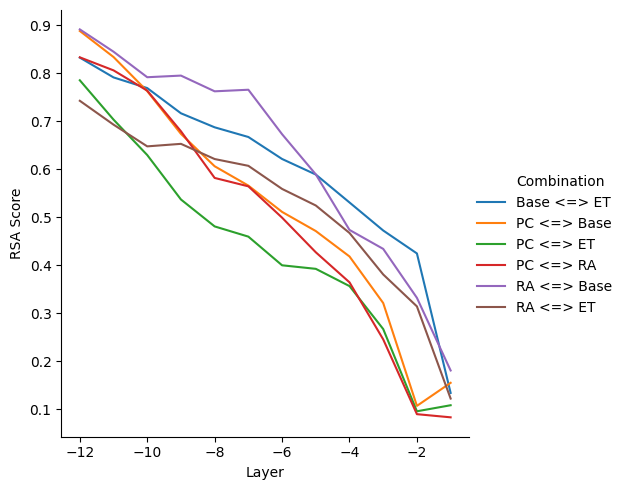
\includegraphics[width=0.5\linewidth]{figures/4_rsa_inter_cls} }\subfloat[Tokens' average\label{fig:rsa-inter-2}]{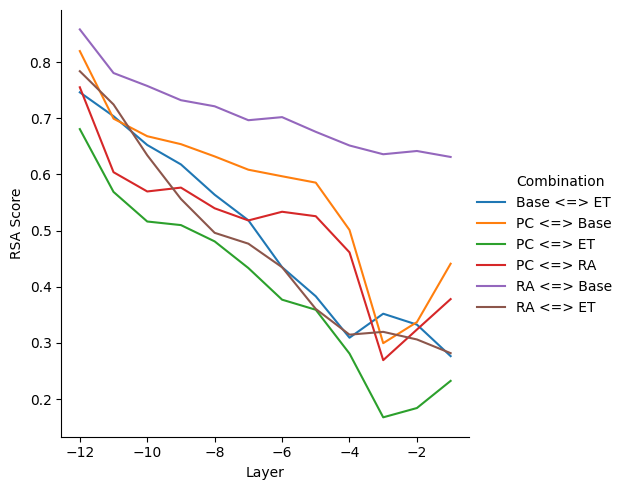
\includegraphics[width=0.5\linewidth]{figures/4_rsa_inter_mean} }\newline\subfloat[All tokens\label{fig:rsa-inter-3}]{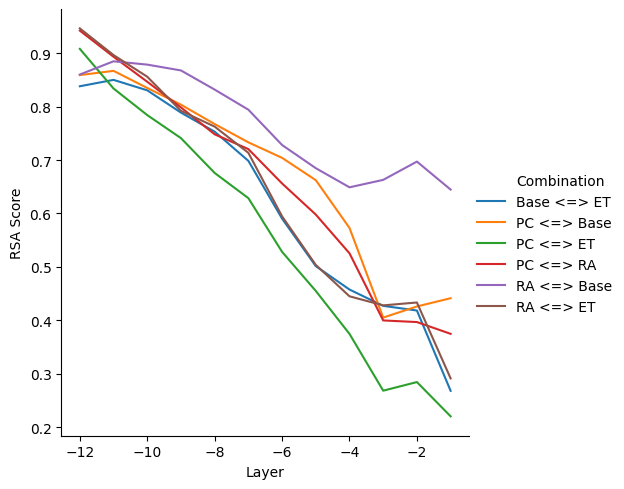
\includegraphics[width=0.5\linewidth]{figures/4_rsa_inter_tokens} }

}

\caption{Inter-model RSA scores across layers for all ALBERT models' combinations. Layer -1 corresponds to the last layer before prediction heads. Higher scores denote stronger inter-model similarity.}\label{fig:rsa-inter}
\end{figure}

The inter-model similarity is evaluated by comparing layer-wise representations of models trained on different tasks using the same ALBERT architecture. Given the representations produced by two ALBERT models trained on different complexity-related annotations for all the sentences in the SST corpus, their similarity is evaluated using both RSA and PWCCA in three settings:

\begin{itemize}
\item
  \textbf{{[}CLS{]} token}: Only the sentence-level \texttt{{[}CLS{]}} initial embedding is considered when evaluating similarity at each layer for all sentences in the SST corpus.
\item
  \textbf{Tokens' average}: A sentence-level embedding obtained by averaging all the individual subword embeddings produced by ALBERT is considered when evaluating similarity at each layer for all sentences in the SST corpus.
\item
  \textbf{All tokens}: The subword embeddings produced by ALBERT for all SST sentences are considered when evaluating similarity at each layer, including \texttt{{[}CLS{]}}, \texttt{{[}SEP{]}} and regular token embeddings, for all sentences in the SST corpus. In practice, the number of considered embedding was set to a maximum of 50,000 to limit such an approach's computational costs.
\end{itemize}

\noindent
Figure \ref{fig:rsa-inter} presents inter-model RSA scores for all model combinations and layers, going from the input layer after initial embeddings (-12) to the last layer before prediction heads (-1).

Given the RSA similarity metric has range \([0,1]\), it can be observed that representational similarity varies greatly across layers, ranging from very high (\(\sim 0.9\)) across bottom layers of the models to very low (\(< 0.1\)) for top layers. This observation supports the widely accepted claim that layers closer to the input in NLMs are almost unaffected by task-specific fine-tuning since they encode low-level properties, while layers closer to prediction heads represent task-related abstract knowledge and tend to diverge rapidly during training.

In settings involving the PC-trained model (yellow, red, and green lines in Figure \ref{fig:rsa-inter}) no sharp decrease in similarity is observed across the top layer for all three variations. Conversely, spikes of decreasing similarity are observed for top layers of all other model pairs. While in terms of \texttt{{[}CLS{]}} all models behave comparably, there is a marked dissimilarity between PC and ET-trained models for top layers when considering all token representations, both with and without averaging (green line in Figures \ref{fig:rsa-inter} a,b). Conversely, RA's \texttt{{[}CLS{]}} representations behave similarly to the ones of other models, but token representations stay very similar to Base even for top layers, i.e.~are slightly affected by fine-tuning (purple line in Figures \ref{fig:rsa-inter} b,c). It can be hypothesized that the RA-trained model cannot collect relevant token-level information since it misses the relative perspective that, as saw in Section \ref{subsubchap:readability}, plays a key role for readability assessment. In this case, PC and ET-trained models are the only ones building relevant complexity-related knowledge, but they still tend to diverge in terms of representational similarity.





\begin{figure}

{\centering \subfloat[CLS token\label{fig:pwcca-inter-1}]{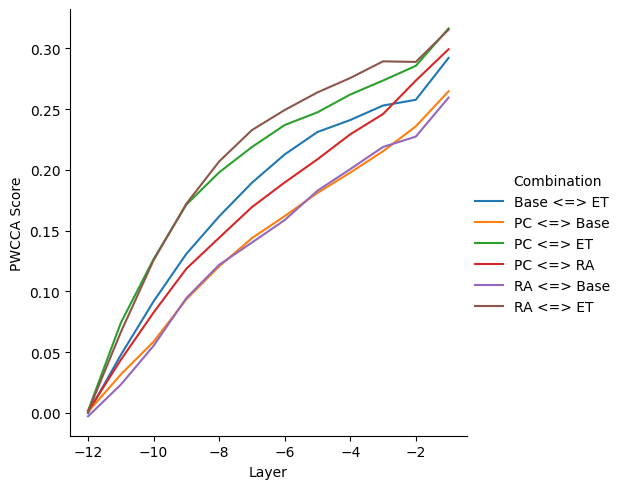
\includegraphics[width=0.5\linewidth]{figures/4_pwcca_inter_cls} }\subfloat[Tokens' average\label{fig:pwcca-inter-2}]{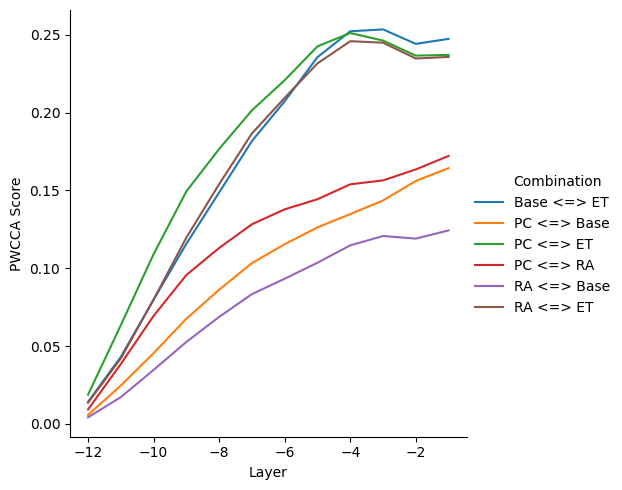
\includegraphics[width=0.5\linewidth]{figures/4_pwcca_inter_mean} }\newline\subfloat[All tokens\label{fig:pwcca-inter-3}]{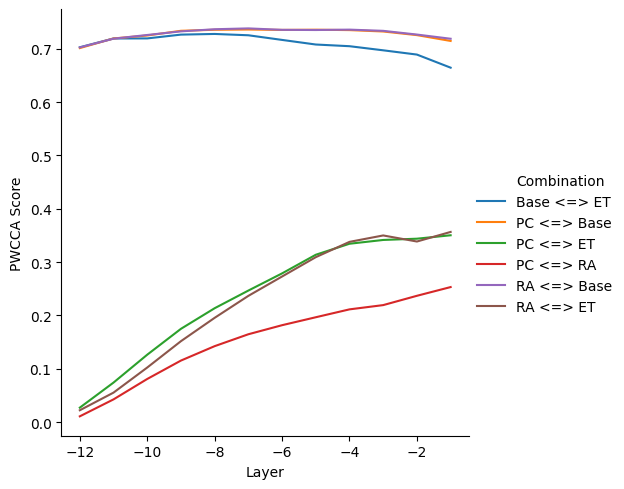
\includegraphics[width=0.5\linewidth]{figures/4_pwcca_inter_tokens} }

}

\caption{Inter-model PWCCA distances across layers for all ALBERT models' combinations. Layer -1 corresponds to the last layer before prediction heads. Higher values denote weaker inter-model similarity.}\label{fig:pwcca-inter}
\end{figure}

Figure \ref{fig:pwcca-inter} presents PWCCA scores in the exact same setup as Figure \ref{fig:rsa-inter}. It does not come as a surprise that scores, in this case, tend to increase while moving towards prediction heads since the PWCCA distance on the \(y\)-axis represents here a function of representational dissimilarity between different layers. Besides this difference, a sharp contrast in behavior is observed in relation to RSA scores, with generally smaller value ranges (\(\sim 0.0\) to \(0.4\)).

In terms of \texttt{{[}CLS{]}} representations, (PC, Base) and (RA, Base) are the two closest pairs, while (PC, ET) and (RA, ET) are furthest. This relation can be rationalized if considering that PC and RA-trained models are trained using the \texttt{{[}CLS{]}} token representation for prediction and have relatively few annotations if compared to the token-level trained ET model. The contrast is even more pronounced when PWCCA distances are measured across token averages (Figure \ref{fig:pwcca-inter} b). Here, pairs containing the ET model quickly diverge from the common trend and settle to a shared PWCCA distance for top layers. Finally, the comparison of all individual token representation contradicts previous RSA trends by showing a remarkably consistent divergence from Base representations at all layers for all the three complexity-trained models.

All in all, both RSA and PWCCA suggest an abstraction hierarchy where the closeness of a representation layer to prediction heads is proportional to the magnitude of changes in parameter values during the training process. While RSA similarity highlights a markedly different behavior for the readability-trained model, the more advanced PWCCA method indicates that representations of models trained with similar objectives stay close in parameter space throughout training, regardless of the conceptual proximity phenomena modeled by their loss functions.

\hypertarget{subsubchap:ex2-intra}{%
\subsection{Intra-model Representational Similarity}\label{subsubchap:ex2-intra}}

The intra-model similarity is evaluated in the same setting of the previous section. However, instead of comparing the same layer across two different models, the representations learned by all layer pairs inside the same model are compared using RSA and PWCCA. Again, the three perspectives of \texttt{{[}CLS{]}}, token's average, and all tokens introduced in the previous chapter are evaluated to understand the shift in representations across layers at different levels of granularity (two sentence-level and one token-level).





\begin{figure}

{\centering \subfloat[CLS token\label{fig:rsa-intra-base-1}]{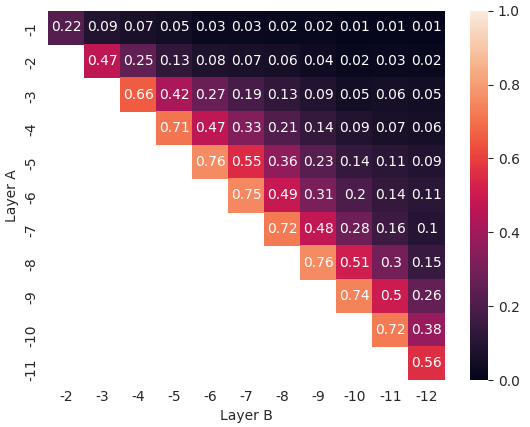
\includegraphics[width=0.5\linewidth]{figures/4_rsa_intra_cls_base} }\subfloat[Tokens' average\label{fig:rsa-intra-base-2}]{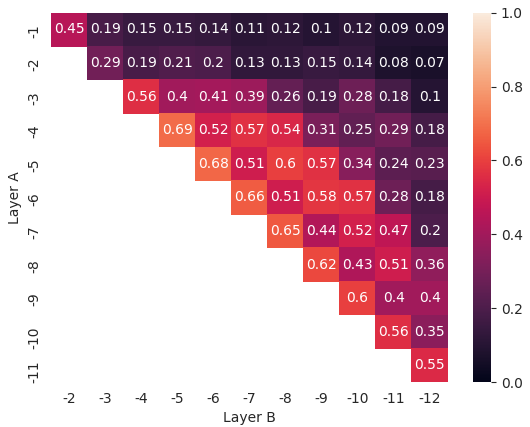
\includegraphics[width=0.5\linewidth]{figures/4_rsa_intra_mean_base} }\newline\subfloat[All tokens\label{fig:rsa-intra-base-3}]{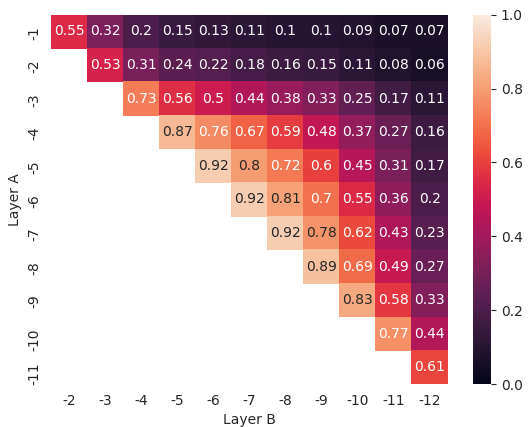
\includegraphics[width=0.5\linewidth]{figures/4_rsa_intra_tokens_base} }

}

\caption{Intra-model RSA scores across layers' combinations for the pre-trained ALBERT model without fine-tuning (\textbf{Base}). Layer -1 corresponds to the last layer before prediction heads. Higher values denote stronger inter-layer similarity.}\label{fig:rsa-intra-base}
\end{figure}

Figure \ref{fig:rsa-intra-base} presents intra-model RSA similarity scores for all layer pairs of the Base model, going from the input layer after initial embeddings (-12) to the last layer before prediction heads (-1). Only the Base model results are presented in this chapter since they are very similar to those produced by fine-tuned models. The latter can be found in Appendix \ref{app:intra-sim}. The first insight relative to RSA intra-model results is that ALBERT layers tend to learn representations that are generally very similar to those of layers in their neighborhood, especially for layers found at the center and close to the input embeddings of the model. While in the case of \texttt{{[}CLS{]}} similarity scores fall sharply beyond the preceding/following layer for each layer, suggesting a significant variation in the information encoded across the model structure, the high-similarity range is much broader for tokens' average and all tokens representations. It is interesting to note that the top two layers (-1 and -2) are almost always very dissimilar in relation to the rest of the model, which is coherent with the spiking behavior around inter-model scores highlighted in the previous section. Another interesting observation is that, while \texttt{{[}CLS{]}} and all tokens' representations are consistently decreasing, the tokens' average representation similarity follows an undulatory behavior across middle layers for all the tested models, with similarity scores dropping and raising while moving away from reference layer. This fact further supports the evidence that token's sentence-level average may better integrate language information from lower layers into high-level representations, as highlighted by \textcite{miaschi-dellorletta-2020-contextual} in the context of morphosyntactic knowledge.





\begin{figure}

{\centering \subfloat[CLS token\label{fig:pwcca-intra-base-1}]{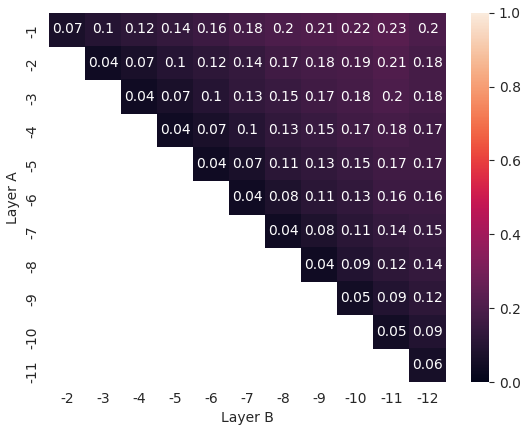
\includegraphics[width=0.5\linewidth]{figures/4_pwcca_intra_cls_base} }\subfloat[Tokens' average\label{fig:pwcca-intra-base-2}]{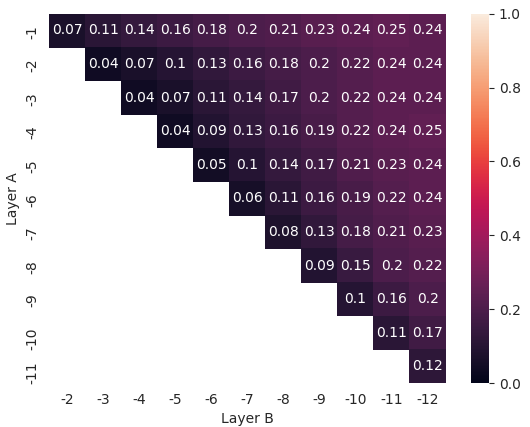
\includegraphics[width=0.5\linewidth]{figures/4_pwcca_intra_mean_base} }\newline\subfloat[All tokens\label{fig:pwcca-intra-base-3}]{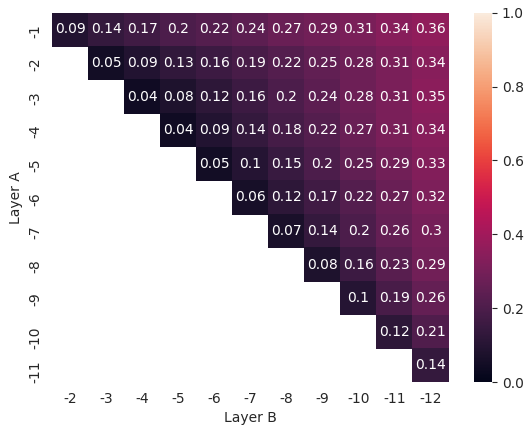
\includegraphics[width=0.5\linewidth]{figures/4_pwcca_intra_tokens_base} }

}

\caption{Intra-model PWCCA distances across layers' combinations for the pre-trained ALBERT model without fine-tuning (\textbf{Base}). Layer -1 corresponds to the last layer before prediction heads. Higher values denote weaker inter-layer similarity.}\label{fig:pwcca-intra-base}
\end{figure}

Figure \ref{fig:pwcca-intra-base} presents PWCCA scores in the exact same setup as Figure \ref{fig:rsa-intra-base}. As in the previous section, the inverse trend in scores here is due to PWCCA being a dissimilarity measure, and the range of result scores is smaller than the one of RSA. Conversely to the previous setting, \texttt{{[}CLS{]}} representations stay closer across layers when their similarity is measured using PWCCA, and there are no significant spikes in score values. The latter finding is coherent with the effect of cross-layer parameter sharing adopted by ALBERT authors. Quoting \textcite{lan-etal-2020-albert}: ``We observe that the transition from layer to layer {[}in terms of L2 distances and cosine similarity{]} are much smoother for ALBERT than for BERT. These results show that weight-sharing affects stabilizing network parameters''. In the context of \texttt{{[}CLS{]}} representations, the lowest layer (-12) appears to be slightly closer to the top layers than the subsequent ones. This fact ultimately supports the intuition that ALBERT is heavily overparametrized, and first-level embeddings already capture much information.

Again for intra-model similarity, PWCCA highlights an abstraction hierarchy inside ALBERT with smoother and generally more reasonable transitions than those showed by RSA. There is no reason to believe that ALBERT adapts its representation hierarchy as a function of its objective since intra-model similarity scores stay approximately the same before and after fine-tuning for all complexity corpora.

\hypertarget{subchap:ex2-summary}{%
\section{Summary}\label{subchap:ex2-summary}}

In this chapter, the representations learned by a neural language model fine-tuned on multiple complexity-related tasks were compared using two widely-used representational similarity approaches. Token and sentence-level representations were compared both considering the same layer across models exposed to different training corpora and different layer pairs contained in the same model. In the first case, the absence of a preponderant similarity between complexity-trained models when compared to the pre-trained one suggests that those models learn their objective by overfitting annotations and without being able to recognize useful primitives that could be recycled throughout complexity tasks. This fact is highlighted in the comparison between perceived complexity and eye-tracking-trained models, where similarity scores of layers close to prediction heads are very different despite the close relationship between the two complexity perspectives. In conclusion, this work strongly supports the claim that representation learning in ALBERT and other neural language models is mainly driven by training biases like task granularity (token-level vs.~sentence-level) that are unrelated to the nature of the task itself. This fact hinders their generalization performances, suggesting that much work still needs to be done beyond language modeling to drive generalizable, hierarchical, and compositional representation learning in models of language.

\hypertarget{chap:ex3}{%
\chapter{\texorpdfstring{\textbf{Gaze-informed Models for Cognitive Processing Prediction}}{Gaze-informed Models for Cognitive Processing Prediction}}\label{chap:ex3}}

\minitoc 

\chaptermark{Gaze-informed Models for Cognitive Processing Prediction}

\begin{quote}
This final experimental chapter aims to study the syntactic generalization capabilities of neural language models by evaluating their performances over atypical linguistic constructions. In particular, architectures pre-trained with masked and causal language modeling are evaluated in their ability to predict garden-path effects on three test suites taken from the SyntaxGym psycholinguistic benchmark. First, the results of previous studies using GPT-2 surprisal to predict garden-path effects are reproduced, and a conversion coefficient is used to evaluate GPT-2 surprisal in terms of human reading times delays. Two neural language models are fine-tuned over gaze metrics from multiple eye-tracking corpora in a multitask token-level setting. Gaze metric predictions on garden-path sentences are evaluated to see whether gaze data fine-tuning can improve garden-path effects prediction. Results highlight how GPT-2 surprisals overestimate the magnitude of MV/RR and NP/Z garden-path effects, and fine-tuning procedures on gaze metrics prediction over typical linguistic structures do not benefit the generalization capabilities of neural language models on out-of-distribution cases like garden-path sentences.
\end{quote}

Human behavioral data collected during naturalistic reading can provide useful insights into the primary sources of processing difficulties during reading comprehension. Multiple cognitive processing theories were formulated to account for the sources of such difficulties (see Section \ref{subchap:garden-path}). Notably, \textbf{surprisal theory} \autocites{hale-2001-probabilistic}{levy-2008-expectation} suggests that processing during reading is the direct result of a single mechanism, that is, the shift in readers' probability distribution over all possible parses. To evaluate whether this perspective holds empirically, language models defining a probability distribution over a vocabulary given previous context (RNNs in \textcite{elman-1991-distributed} and \textcite{mikolov-etal-2010-recurrent}, recently Transformers in \textcite{hu-etal-2020-systematic}) are commonly used to obtain accurate predictability estimates that can directly be compared to behavioral recordings (e.g.~gaze metrics) acting as proxies of human cognitive processing.

A computational model that consistently mimics human processing behaviors would provide strong evidence of cognitive processing's underlying probabilistic-driven nature. For this reason, many studies in the fields of syntax and psycholinguistics have focused on probing the abilities of language models to highlight phenomena related to reading difficulties \autocites{linzen-etal-2016-assessing}{gulordava-etal-2018-colorless}{futrell-etal-2019-neural}. Peculiar constructions like garden-path sentences are often used in this context to evaluate the generalization capabilities of language models for two main reasons. First, garden-path sentences are rare in naturally-occurring text. As such, they represent out-of-distribution examples for any language model trained on conventional data and can be used to test the latter's generalization capabilities. Secondly, researchers nowadays have access to reasonably-sized literature describing the impact of garden-path effects on cognitive processing proxies such as gaze recordings, with articles being often released alongside publicly-available resources for reproducible evaluation \autocites{prasad-linzen-2019-self}{prasad-linzen-2019-much} and recently even ad-hoc benchmarks \autocite{gauthier-etal-2020-syntaxgym}.

This final experimental chapter evaluates the ability of neural language models in predicting garden-path effects observed on human subjects, using language modeling surprisal and eye-tracking metrics elicited respectively before and after multitask token-level eye-tracking fine-tuning for garden-path effects prediction. Specifically, an autoregressive (GPT-2, \textcite{radford-etal-2019-language}) and a masked language model (ALBERT, \textcite{lan-etal-2020-albert}) are first tested over three garden-path test suites that are part of the SyntaxGym benchmark to evaluate whether their language modeling surprisal before and after eye-tracking fine-tuning (ET) can be used to predict the presence and the magnitude of garden-path effects over disambiguating regions. In particular, GPT-2 and GPT-2 XL results presented in \textcite{hu-etal-2020-systematic} are reproduced. Finally, the same procedure is repeated using predicted eye-tracking scores predicted by models after fine-tuning instead of language modeling surprisal, following the intuition that an accurate model of gaze measurements should predict such phenomena correctly.

While the usage of surprisal is a common practice for garden-path effect prediction, leveraging eye-tracking scores predicted by a neural language model trained for this purpose is a novel research direction that is deemed interesting as a way to combine the predictive power of modern language models and the strong connection between cognitive processing and gaze metrics. While predicted gaze metrics for garden-path evaluation were used in concurrent studies \autocite{schjindel-linzen-2020-single}, the approach adopted by this work can be regarded as complementary evidence since eye-tracking metrics predictions are produced as results of an end-to-end supervised fine-tuning procedure involving a neural language model rather than being derived from surprisal values through a conversion coefficient. Findings suggest that, while surprisal scores from autoregressive models accurately reflect garden-path structures both before and after fine-tuning, gaze metrics predictions produced by fine-tuned models do not account for the temporary syntactic ambiguity that characterizes such sentences and makes them difficult to process.

\paragraph{Contributions} This study validates the performances of standard and gaze-informed Transformed-based neural language models for garden-path effects prediction. In particular:

\begin{itemize}
\item
  It reproduces the GPT-2 performances on garden-path test suites reported by \textcite{gauthier-etal-2020-syntaxgym} and highlights how GPT-2 overestimates reading delays caused by garden-path effects on MV/RR and NP/Z constructions.
\item
  It highlights masked language models' inability to consistently predict garden-path effects, using language modeling surprisal and gaze metrics predictions.
\item
  It introduces a novel gaze metrics multitask token-level fine-tuning approach that, despite being accurate for predicting eye-tracking scores on standard constructions, does not improve models' performances on garden-path effects predictions.
\end{itemize}

\hypertarget{subchap:ex3-setup}{%
\section{Experimental Setup}\label{subchap:ex3-setup}}

\paragraph{Fine-tuning data} As for the gaze metrics model presented in the previous chapter, all eye-tracking datasets presented in Section \ref{subsubchap:eye-tracking} were merged and used to fine-tune neural language models using the multitask token-level approach described in Appendix \ref{app:et-modeling}. Only the training variant without embedding concatenation (referred to as ``surprisal'' in the appendix) was evaluated on garden-path test suites given comparable modeling performances.

\paragraph{Models} Two variants of GPT-2 having respectively 117 million and 1.5 billion parameters are evaluated in terms of surprisal-driven predictability, alongside an ALBERT model with 11 million parameters.\footnote{The \texttt{gpt2}, \texttt{gpt2-xl} and \texttt{albert-base-v2} pre-trained models from 🤗 \texttt{transformers} \autocite{wolf-etal-2020-huggingface}.} Only the small GPT-2 model and the ALBERT model were fine-tuned for gaze metric predictions due to limited computational resources.

\paragraph{Evaluation data} SyntaxGym \autocite{gauthier-etal-2020-syntaxgym} is a recently introduced online platform designed to make the targeted evaluation of language models on psycholinguistic test suites both accessible and reproducible. The MV/RR and NP/Z test suites containing garden paths from \textcite{futrell-etal-2019-neural} are used in the context of this work. The MV/RR test suite consists of 28 groups containing a sentence with a main verb/reduced relative ambiguity and its non-ambiguous rewritings. In comparison, the NP/Z test suites consist of 24 groups containing a sentence with a nominal/zero predicate ambiguity, produced either by a misinterpreted transitive use of a verb (Verb Transitivity) or the absence of an object for the main verb (Overt Object). Examples (3), (4), and (5) from Section \ref{subchap:garden-path} follow the format used in the three SyntaxGym test suites used in this work.





\begin{figure}

{\centering \subfloat[NP/Z Ambiguity (Verb Transitivity)\label{fig:gpt2-surprisal-1}]{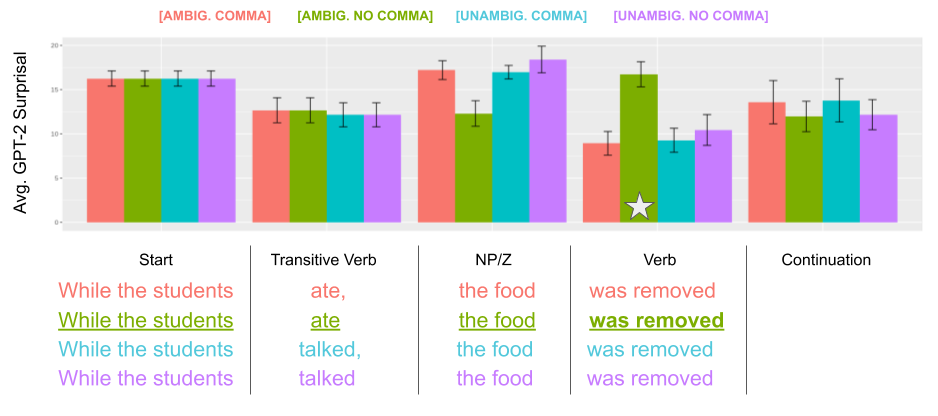
\includegraphics[width=1\linewidth]{figures/5_gpt2_surprisal_npz_ambig} }\newline\subfloat[NP/Z Ambiguity (Overt Object)\label{fig:gpt2-surprisal-2}]{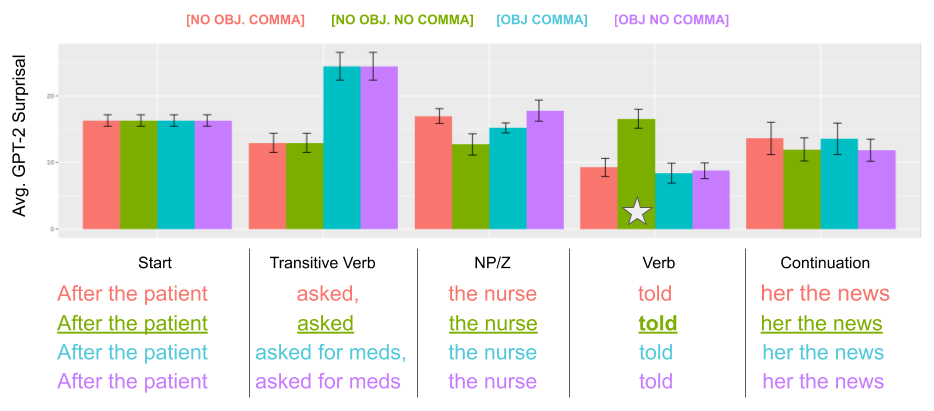
\includegraphics[width=1\linewidth]{figures/5_gpt2_surprisal_npz_obj} }\newline\subfloat[MV/RR Ambiguity\label{fig:gpt2-surprisal-3}]{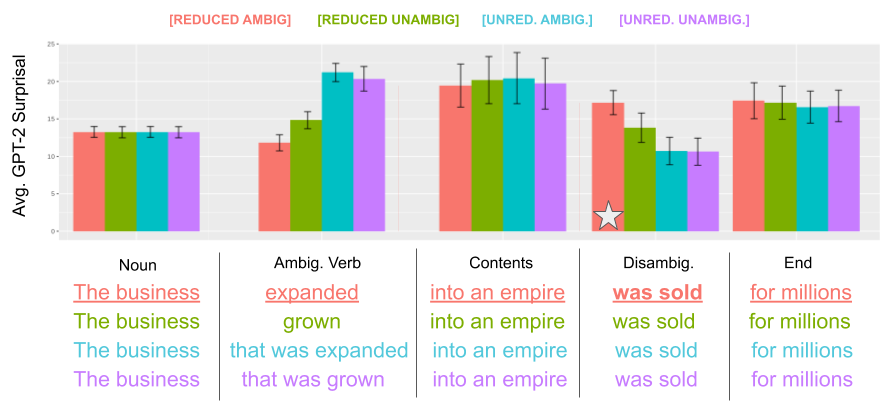
\includegraphics[width=1\linewidth]{figures/5_gpt2_surprisal_mvrr} }

}

\caption{Average GPT-2 surprisal predictions and examples for the three SyntaxGym test suites. Star marks the garden-path disambiguator (bold in examples), and bars show 95\% confidence intervals.}\label{fig:gpt2-surprisal}
\end{figure}

\hypertarget{subchap:ex3-experiments}{%
\section{Experimental Evaluation}\label{subchap:ex3-experiments}}

For the first part of the experiments, the smallest version of the model GPT-2 is used. Figure \ref{fig:gpt2-surprisal} reproduces the original setting tested by \textcite{hu-etal-2020-systematic}, showing how predictability estimates produced by the model correctly individuate the presence of garden-path effects.\footnote{Similar plots are available on the SyntaxGym website: \url{http://syntaxgym.org/viz/individual}} Surprisal values are computed using a pre-trained GPT-2 for all tokens in all sentences of the three test suites. Then, those values are aggregated by summing them across all tokens composing a sentence region. For example, for the NP/Z Ambiguity test suite entry shown in example (a) the region ``Start'' will be associated with the sum of surprisal estimates for all subword tokens in the sequence \emph{While the students}. It is important to note that the four variants of the same sentence have only minimal variations, but only one of those (the underlined one in all examples) is a garden-path sentence. After computing GPT-2 surprisal scores for all regions of all sentences in the test sets, those are averaged region-wise across sentences belonging to the same test set to obtain the three plots presented in Figure \ref{fig:gpt2-surprisal}. The star symbol is used to mark the disambiguating region of garden-path sentences, making evident how predictability estimates are significantly lower (i.e., higher surprisal values) for those and correctly predict the presence of a garden-path effect in most settings and for all the three garden-path variants.

\hypertarget{subsubchap:ex3-magnitudes}{%
\subsection{Estimating Magnitudes of Garden-path Delays}\label{subsubchap:ex3-magnitudes}}

An important part of evaluating model predictions over garden-path sentences is determining whether the increase in surprisal scores correctly captures the effect's magnitude. \textcite{schjindel-linzen-2020-single} perform this evaluation on RNN language models, finding that they vastly underestimate garden-path effects for MV/RR and NP/Z ambiguities. In their approach, \textcite{schjindel-linzen-2020-single} estimate the surprisal-to-reading-times conversion rate at 2ms per surprisal bit by fitting a linear mixed-effect model on relevant factors (surprisal, entropy, word length, among others) relative to a word and its three preceding words to account for spillover effects. The approach adopted in this work is different in that it stems from the empirical relation between surprisal scores produced by GPT-2 and reading times produced by eye-tracking experiments' participants. Figure \ref{fig:surprisal-ratios} presents the median values over words for the ratio between gaze metrics recorded by participants and GPT-2 surprisal estimates, with the red cross indicating the average median surprisal-to-metric ratio \(C_{\text{corpus}}^{\text{metric}}\) computed across all participants of a corpus. The following formula is used to produce the surprisal-to-reading-times conversion coefficient:
\begin{equation}
C_{S\rightarrow RT} = w_1 \cdot C_{\text{GECO}}^{\text{FPD}} + w_2 \cdot C_{\text{Dundee}}^{\text{FPD}} + w_3 \cdot C_{\text{ZuCo NR}}^{\text{FPD}} + w_4 \cdot C_{\text{ZuCo SR}}^{\text{FPD}} + w_5 \cdot C_{\text{ZuCo 2.0}}^{\text{FPD}}
\end{equation}
with \(w = [.4, .45, .05, .05, .05]\) being the weighting coefficients representing the proportion of each corpus' tokens over the total amount of available gaze-annotated tokens.



\begin{figure}

{\centering 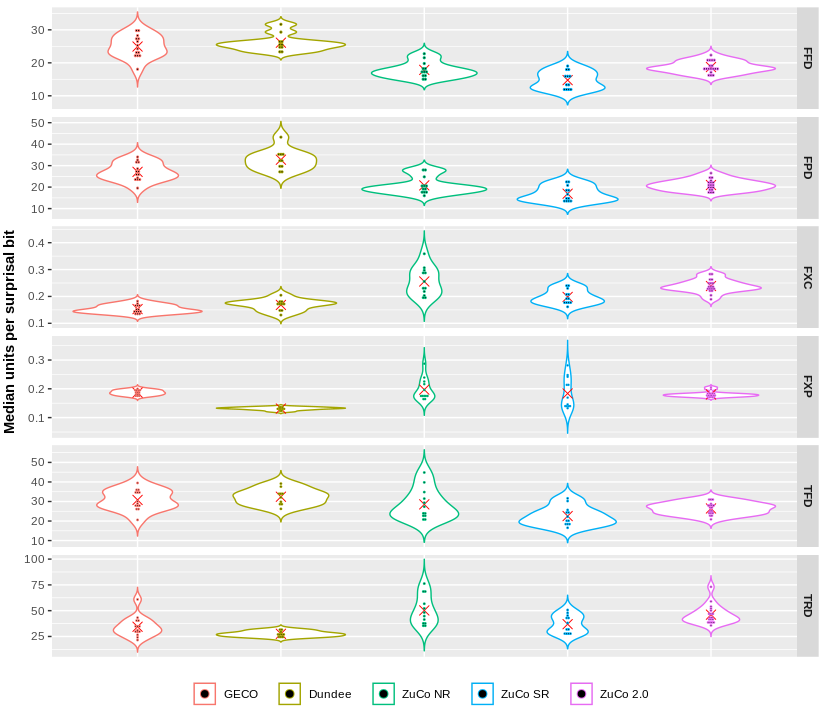
\includegraphics[width=1\linewidth]{figures/5_surprisal_ratios} 

}

\caption{Median scores for the ratio between gaze metrics units and GPT-2 surprisal estimates across all participants of all eye-tracking datasets used in this study. The red cross shows the average across participants of a single dataset. Units are in ms for durations, \% for FXP, and raw counts for FXC.}\label{fig:surprisal-ratios}
\end{figure}

The resulting value for the conversion coefficient is \(27.7\), i.e., \emph{each surprisal bit predicted by GPT-2 accounts for roughly 27.7 milliseconds in first pass duration} (30.3ms using TFD). When applied to the average effects predicted by GPT-2 in Figure \ref{fig:gpt2-surprisal}, it leads to an estimated delay of roughly 64ms for the MV/RR setting and 166ms and 194ms for the NP/Z Ambiguity and NP/Z Overt Object settings, respectively. These computed delays overestimate the literature's effects: \textcite{prasad-linzen-2019-self} and \textcite{prasad-linzen-2019-much}, for example, report an average garden-path effect of 22ms and 27ms for MV/RR and NP/Z variants, respectively. However, it should be mentioned that precedent studies found higher delays for NP/Z structures: \textcite{grodner-etal-2003-against} find a 64ms delay on disambiguating words, and \textcite{sturt-etal-1999-structural}`s delays of 152ms per word are close to the estimates produced by GPT-2 surprisal predictions. Overall, using models' surprisal on gaze-annotated sentences to directly compute a conversion coefficient produces values that correctly identify delays on disambiguating regions and overestimate the magnitude of garden-path effects conversely to what was found by \textcite{schjindel-linzen-2020-single}. Even with an adjustment of the conversion coefficient to match MV/RR estimates with \textcite{prasad-linzen-2019-self} findings, the NP/Z effect prediction would still be much larger than the empirically-observed values collected in comparable settings.

\hypertarget{subsubchap:ex3-predicting}{%
\subsection{Predicting Delays with Surprisal and Gaze Metrics}\label{subsubchap:ex3-predicting}}

The other perspective explored in this study is evaluating whether gaze metric predicted by models fine-tuned on eye-tracking corpora annotations can correctly estimate the presence and magnitude of garden-path effects and how they compare to surprisal-driven approaches. Table \ref{tab:gp-results} presents the accuracy of multiple pre-trained Transformer-based language models in respecting a set of three conditions taken from \textcite{hu-etal-2020-systematic} for each SyntaxGym test suite, namely:
\begin{equation}
V_d(b) < V_d(a);\qquad V_d(c) < V_d(a);\qquad V_d(c)-V_d(d) < V_d(a)-V_d(b)
\end{equation}
Where \(V_d(a)\) corresponds to the value, either in terms of surprisal or gaze metrics, assigned by a model to the disambiguating region \(d\) of sentence \(a\), and \(a,b,c,d\) are the same sentence's variants for each test suite presented in examples (3),(4) and (5) of Section \ref{subchap:garden-path}. Accuracy is computed as the proportion of items in the test suite on which the language model's predictions conform to the respective criterion. The first three models (GPT-2, GPT-2 XL, and ALBERT) are the pre-trained variants of the three models presented in Table \ref{subchap:ex3-setup} without additional fine-tuning. Instead, the GPT-2 ET and ALBERT ET models correspond to the same GPT-2 and ALBERT models as before after a multitask token-level fine-tuning on gaze metrics for all the aggregated corpora. The top part of Table \ref{tab:gp-results} shows the five models' performances while using region-aggregated surprisals as predictors. Focusing on the GPT-2 variants, it can be observed that they all achieve considerably high scores on all evaluated conditions. Conversely, ALBERT masked language models poorly fit the specified criteria. This fact can be intuitively explained by accounting for the different training and evaluation setup used for the two architectures. GPT-2 models are likely to produce high surprisal estimates for garden-path sentences since, processing the input autoregressively and having access only to previous tokens, they incur in the same syntactic ambiguities faced by human readers.

\begin{landscape}\begin{table}[!h]

\caption{\label{tab:gp-results}Results of experiments using surprisal and gaze metrics as predictors for garden-path effects on the three SyntaxGym test suites.}
\centering
\fontsize{11}{13}\selectfont
\begin{threeparttable}
\begin{tabular}[t]{lllcc>{}c|cc>{}c|ccc}
\toprule
\multicolumn{1}{c}{\textbf{}} & \multicolumn{1}{c}{\textbf{}} & \multicolumn{1}{c}{\textbf{}} & \multicolumn{3}{c}{\textbf{NP/Z Verb Transitivity}} & \multicolumn{3}{c}{\textbf{NP/Z Overt Object}} & \multicolumn{3}{c}{\textbf{MV/RR Ambiguity}} \\
\cmidrule(l{3pt}r{3pt}){4-6} \cmidrule(l{3pt}r{3pt}){7-9} \cmidrule(l{3pt}r{3pt}){10-12}
 &  &  & Cond.  1 \textsuperscript{1} & Cond.  2 \textsuperscript{2} & Cond.  3 \textsuperscript{3} & Cond.  1 \textsuperscript{a} & Cond.  2 \textsuperscript{b} & Cond.  3 \textsuperscript{c} & Cond.  1 \textsuperscript{*} & Cond.  2 \textsuperscript{\dag} & Cond.  3 \textsuperscript{\ddag}\\
\midrule
\addlinespace[0.3em]
\multicolumn{12}{l}{\textbf{Surprisal}}\\
\hspace{1em} & GPT-2 &  & 0.96 & 0.92 & 0.88 & \textbf{0.96} & \textbf{1} & \textbf{1} & \textbf{1} & \textbf{0.89} & \textbf{0.82}\\
\cmidrule{2-12}
\hspace{1em} & GPT-2 XL &  & \textbf{1} & \textbf{0.96} & \textbf{1} & \textbf{0.96} & \textbf{1} & \textbf{1} & 0.93 & 0.75 & 0.75\\
\cmidrule{2-12}
\hspace{1em} & ALBERT &  & 0.21 & 0.63 & 0.58 & 0.21 & 0.54 & 0.46 & 0.61 & 0.54 & 0.38\\
\cmidrule{2-12}
\hspace{1em} & GPT-2 ET &  & 0.96 & 0.88 & 0.79 & \textbf{0.96} & \textbf{1} & 0.96 & 0.96 & 0.79 & \textbf{0.82}\\
\cmidrule{2-12}
\hspace{1em} & ALBERT ET &  & 0.42 & 0.42 & 0.58 & 0.42 & 0.75 & 0.62 & 0.5 & 0.64 & 0.64\\
\cmidrule{1-12}
\addlinespace[0.3em]
\multicolumn{12}{l}{\textbf{Eye-tracking metrics}}\\
\hspace{1em} & GPT-2 ET & FFD & 0.29 & 0.38 & 0.46 & 0.29 & 0.54 & 0.42 & 0.86 & 0.57 & 0.5\\

\hspace{1em} &  & FPD & 0.13 & 0.46 & 0.67 & 0.13 & 0.5 & 0.46 & 0.86 & 0.54 & 0.36\\

\hspace{1em} &  & FXP & 0.38 & 0.5 & 0.42 & 0.42 & 0.41 & 0.42 & 0.71 & 0.43 & 0.57\\

\hspace{1em} &  & FXC & 0.75 & 0.5 & 0.42 & 0.75 & 0.63 & 0.46 & 0.92 & 0.46 & 0.54\\

\hspace{1em} &  & TFD & 0.5 & 0.33 & 0.46 & 0.5 & 0.58 & 0.75 & 0.79 & 0.43 & 0.39\\

\hspace{1em} &  & TRD & 0.67 & 0.46 & 0.54 & 0.63 & 0.25 & 0.54 & 0.29 & 0.39 & 0.5\\
\cmidrule{2-12}
\hspace{1em} & ALBERT ET & FFD & 0.67 & 0.33 & 0.42 & 0.42 & 0.83 & 0.67 & 0.68 & 0.61 & 0.5\\

\hspace{1em} &  & FPD & 0.54 & 0.41 & 0.33 & 0.38 & 0.79 & 0.75 & 0.75 & 0.57 & 0.46\\

\hspace{1em} &  & FXP & 0.28 & 0.46 & 0.29 & 0.54 & 0.38 & 0.63 & 0.29 & 0.5 & 0.43\\

\hspace{1em} &  & FXC & 0.63 & 0.46 & 0.5 & 0.38 & 0.67 & 0.71 & 0.86 & 0.43 & 0.39\\

\hspace{1em} &  & TFD & 0.75 & 0.38 & 0.29 & 0.5 & 0.88 & 0.83 & 0.79 & 0.61 & 0.54\\

\hspace{1em} &  & TRD & 0.96 & 0.42 & 0.42 & 0.63 & 0.75 & 0.5 & 0.79 & 0.5 & 0.57\\
\bottomrule
\end{tabular}
\begin{tablenotes}[para]
\small
\item Description of the evaluated conditions
\item \underline{\textit{NP/Z Verb Trans.: }} 
\item[1] [Ambig. No Comma] > [Ambig. Comma]; 
\item[2] [Ambig. No Comma] > [Unambig. No Comma]; 
\item[3] [Ambig. No Comma] - [Ambig. Comma] > [Unambig. No Comma] - [Unambig. Comma]
\item \underline{\textit{NP/Z Overt Obj.: }} 
\item[a] [No Obj. No Comma] > [No Obj. Comma]; 
\item[b] [No Obj. No Comma] > [Obj. No Comma]; 
\item[c] [No Obj. No Comma] - [No Obj. Comma] > [Obj. No Comma] - [Obj. Comma]
\item \underline{\textit{MV/RR Ambig.: }} 
\item[*] [Reduced Ambig.] > [Unred. Ambig.]; 
\item[\dag] [Reduced Ambig.] > [Reduced Unambig.]; 
\item[\ddag] [Reduced Ambig.] - [Unred. Ambig.] > [Reduced Unambig.] - [Unred. Unambig.]
\end{tablenotes}
\end{threeparttable}
\end{table}
\end{landscape}

Conversely, ALBERT-like masked language models have access to bidirectional contexts and are not exposed to the ambiguity. It is interesting to observe that while the eye-tracking fine-tuning procedure appears to hamper GPT-2 surprisal performances, it generally improves the ALBERT model's accuracy. This phenomenon may be due to the sequential nature of reading that is being captured by gaze metrics and transferred to the bidirectional ALBERT model as a useful bias for sequential processing. The same procedure performs suboptimally, instead, when associated with an inherently autoregressive model like the GPT-2 decoder

The bottom part of Table \ref{tab:gp-results} presents the two ET-trained models' accuracy in matching criteria using predicted gaze metrics. For both GPT-2 and ALBERT, it can be observed that gaze metrics vastly underperform in accuracy terms. We can conclude that, despite the conceptual relation between gaze metrics and predictability observed in humans, the predictions of fine-tuned model cannot generalize to unseen settings, and as such \emph{eye-tracking predictions obtained after a fine-tuning on standard constructions do not appear useful to individuate or estimate the magnitude of garden-path effects}. This observation suggests that fine-tuned models stick to predicting gaze metric values that are the most likely for each specific token, regardless of the surrounding context's ambiguities. Plots in Appendix \ref{app:garden-paths-et} present the region-aggregated average scores for all metrics predicted by GPT-2 ET in the same format as before and show how predictions on the disambiguator regions are unaffected by the presence of previous ambiguities.

\hypertarget{subchap:ex3-summary}{%
\section{Summary}\label{subchap:ex3-summary}}

This chapter focused on two perspectives related to the evaluation of neural language models for garden-path effects prediction. First, promising results from previous studies using GPT-2 surprisal to evaluate predictability are reproduced, and language modeling surprisal estimates are converted to reading times using a conversion coefficient. Resulting predictions vastly overestimate the magnitude of garden-path effects in all settings, suggesting the presence of additional mechanisms besides predictability in shaping cognitive processing in the presence of ambiguous constructions like garden-path sentences. This evidence is further supported by the second experimental perspective, in which reading times for garden-path sentences are predicted by models fine-tuned on eye-tracking annotations on corpora containing standard constructions. Results suggest that predicted gaze metrics poorly estimate the presence of garden-path effects over disambiguating regions, suggesting that fine-tuned models are once again incapable of out-of-the-box generalization beyond training settings.

\hypertarget{conclusion}{%
\chapter*{\texorpdfstring{\textbf{Conclusion}}{Conclusion}}\label{conclusion}}
\addcontentsline{toc}{chapter}{\textbf{Conclusion}}

\markboth{Conclusion}{}

This thesis work adopted a model-driven approach to investigate the relationship between different linguistic complexity perspectives for the English language and study how those are learned and encoded by deep learning models at various abstraction levels.

From the theoretical viewpoint of connecting different complexity perspectives using empirical annotations, Chapter \ref{chap:ex1} analysis highlighted the strong connection between online/offline complexity metrics and length-related linguistic properties of sentences. The relation was further investigated in length-controlled settings, obtaining similar results across online gaze measurements but different for offline perceived complexity annotations. The overall results identify syntagmatic complexity as the primary source of variation in both offline and online complexity perception for readers. However, they also show how the variety in parts and hierarchical structures contributes differently across different complexity perspectives when sentence length is controlled. Another theoretical aspect supported by Chapter \ref{chap:ex3} experimental results is the role played by cognitive mechanisms other than predictability in shaping human processing patterns on ambiguous constructions like garden-path sentences. In this context, a computational model that accurately predicts the presence or garden-path effects was used as a psycholinguistic subject to provide predictability annotations on standard and atypical constructions. A surprisal-to-reading-times conversion coefficient was then estimated from gaze annotations and surprisal scores on standard constructions. The resulting reading times were used to highlight how the model widely overestimated the magnitude of garden-path effects, following the methodology of \textcite{schjindel-linzen-2020-single}. While results differ significantly from the latter study due to a much larger conversion coefficient, the presence of different accounts for cognitive processing is supported when considering how proportions in predicted magnitudes on different types of constructions do not match the ones reported in recent psycholinguistics literature.

Despite interesting theoretical findings, this work is mostly devoted to interpreting complexity phenomena from a modeling standpoint. Chapter \ref{chap:ex1} evaluates the encoding of linguistic properties inside neural language models' representations using probing tasks performed before and after model fine-tuning on complexity-related tasks. Results highlighted the emergence of task-related linguistic properties within the model's representations after the fine-tuning process, providing evidence for the relation between models' linguistic skills during training and their performances on morphosyntactically-related tasks. In light of these findings, it can be conjectured that linguistic probes may provide a reasonable estimate of the task-oriented quality of representations for those highly-syntactic tasks. In Chapter \ref{chap:ex2}, the representations learned by neural language models were compared across layers and fine-tuning tasks using representational similarity approaches. The absence of higher similarity scores between complexity-trained models compared to the pre-trained one suggests that training objectives are learned by overfitting annotations and that learned parameters hardly capture information that could be relevant for multiple complexity-related tasks.

Moreover, task framing and the annotation modalities were observed to play a much larger role in defining representational similarity scores rather than the conceptual similarity between tasks. This fact supports the claim that standard optimization procedures used in deep learning are not suitable for this type of concept-driven learning. Finally, Chapter \ref{chap:ex3} highlighted the inability of standard neural language models in leveraging syntactic cues to improve prediction in the context of garden-path effects. Models fine-tuned on gaze annotations were tested on garden-path test suites to evaluate whether reading time predictions can perform as well as surprisal in identifying garden-path triggers. Results highlight how models heavily overfit gaze annotation and cannot predict the increase in reading times observed in human subjects despite being exposed to the temporary syntactic ambiguity that characterizes garden-path constructions.

Recent trends in transfer learning have profoundly shaped the last few years of research in NLP, leading to astonishing improvements in almost all language-related tasks, including linguistic complexity prediction. Despite all the hype, the fundamental problem behind all computational linguistics research remains: even the most powerful deep learning models do not ``understand'' language, and their learned representations are ``potentially useful, but incomplete, reflections of the actual meaning'' they derive from structural training procedures \autocite{bender-koller-2020-climbing}. In support of this affirmation, all models leveraged in this study by following closely standard procedures were found lacking in generalization capabilities and hierarchical abstraction, despite their excellent performances on predicting in-domain observations. To conclude with a somewhat cliché affirmation, much work still needs to be done to drive generalizable, hierarchical, and compositional representation learning in language models, enabling proper human-level natural language understanding.

\hypertarget{broader-impact-and-ethical-perspectives}{%
\section*{Broader Impact and Ethical Perspectives}\label{broader-impact-and-ethical-perspectives}}
\addcontentsline{toc}{section}{Broader Impact and Ethical Perspectives}

The findings described in this thesis work are mostly meta-analytical, and as such, mostly intended to distill theoretical insights and evaluate recent efforts in the natural language processing community. This said, some of the models and procedures described in this work can be clearly beneficial to society. For example, using models trained to predict reading patterns may be used in educational settings to identify difficult passages that can be simplified, improving reading comprehension for students in a fully-personalizable way. This type of technology can also be applied to domain-specific documents such as juridical or medical reports to identify critical areas that can be adapted to improve layman's understanding. However, it is essential to recognize the potentially malicious usage of such systems. The integration of eye-tracking systems in mobile devices, paired with predictive models presented in this work, could be used to build harmful surveillance systems and advertisement platforms using gaze predictions for extreme behavioral manipulation. Moreover, multiple individuals' gaze data could be leveraged by autonomous systems to enforce discriminatory practices towards neurodiverse subjects in hardly-detectable ways. In terms of research impact, the experiments presented in this work may provide useful insights into the behavior of neural language models for researchers working in the fields of interpretability in NLP and computational psycholinguistics.

\hypertarget{future-directions}{%
\section*{Future Directions}\label{future-directions}}
\addcontentsline{toc}{section}{Future Directions}

In conclusion, multiple paths to improve and extend the scope of this work were identified during the experimental process, and will be left here as a final note for my future self and for anyone interested in pushing forward research in fields related to this thesis' topics.

\begin{itemize}
\item
  Self-training has recently proven to be very effective for compensating the lack of large labeled datasets in the context of acceptability and complexity prediction \autocite{sarti-2020-umbertomtsa}. In light of these results, it would be interesting to evaluate whether self-training could also improve the performances and generalization of models used for gaze metrics prediction.
\item
  Evaluate whether gaze-trained neural language models having undergone a \emph{cloze distillation process} \autocite{eisape-etal-2020-cloze}, combining intuitions from masked language modeling and knowledge distillation \autocite{hinton-etal-2015-distilling}, would produce better results for modeling out-of-distribution garden-path phenomena compared to the somewhat naive approach adopted in this study.
\item
  Incorporating gaze metrics prediction in the training objectives of learning models can be interesting to account for human cognitive biases during reading. The crucial aspect is how to get a sufficient amount of annotated data to make this idea scalable for modern language models' pre-training needs. In this regard, it could be interesting to test the approach by \textcite{hollenstein-zhang-2019-entity} where mean gaze scores are averaged for each type across annotators, effectively providing a way to label input sentences with robust gaze information in an unsupervised manner.
\item
  Since eye-tracking metrics are complexity signals with free human supervision, it could be possible to leverage those for simplification and other related tasks in an iterative learning-from-human-feedback paradigm similar to the one described in \textcite{stiennon-etal-2020-learning}.
\item
  It should in principle be possible to use human processing data as a replacement for the self-attention computation. The dot product critically bounds the computational efficiency of attention-based models, and fixed attention has been shown to have a limited negative impact on final results while making inference much faster \autocite{tay-etal-2020-synthesizer}. Fixing attention weights using human attention, as measured by eye-tracking metrics, can be an exciting perspective to explore in this context. This idea can be thought of as an application of human attention regularization of LSTM attentional networks for various tasks proposed in \textcite{barrett-etal-2018-sequence} to Transformers networks.
\item
  Would explicitly embedding complexity in the learning process of language models favor hierarchical abstraction? In this perspective, it would be exciting to evaluate whether a model trained on easy-to-hard sentences following language acquisition insights would encode different knowledge in terms of linguistic structures, concept abstraction, and allowances.
\item
  Finding better ways to instill useful inductive biases into learning models, especially for syntax-heavy downstream tasks. Concrete examples following this direction may use parsing as a complementary task to keep top-level representations sensible to syntactic changes, as tested in \textcite{glavas-vulic-2020-supervised} for natural language understanding, or use hybrid symbolic-neural models to represent syntax as in \textcite{zanzotto-etal-2020-kermit}.
\end{itemize}

\startappendices

\hypertarget{app:ling-feats}{%
\chapter{Linguistic Features}\label{app:ling-feats}}

The following list of features was used in the context of Chapter \ref{chap:ex1} experiments and is a summary of the full set of features presented in \textcite{brunato-etal-2020-profiling}:

\hypertarget{raw-text-properties-and-lexical-variety}{%
\section{Raw Text Properties and Lexical Variety}\label{raw-text-properties-and-lexical-variety}}

\begin{itemize}
\item
  \textbf{Sentence length} (\emph{n\_tokens}): Length of the sentence in terms of number of tokens.
\item
  \textbf{Word length} (\emph{char\_per\_tok}): Average number of characters per word in a sentence, excluding punctuation.
\item
  \textbf{Type/Token Ratio for forms and lemmas} (\emph{ttr\_form, ttr\_lemma}): Ratio between the number of lexical types and the number of tokens within a sentence.
\end{itemize}

\hypertarget{morpho-syntacting-information}{%
\section{Morpho-syntacting Information}\label{morpho-syntacting-information}}

\begin{itemize}
\item
  \textbf{Distribution of grammatical categories} (\emph{upos\_dist\_*, xpos\_dist\_*}): Percentage distribution in the sentence of the 17 core part-of-speech categories present in the Universal POS tagset (adjective, adverb, interjection, noun, proper noun, verb, adposition, auxiliary, coordinating conjunction, determiner, numeral, particle, pronoun and subordinating conjunction, punctuation, and symbols).
\item
  \textbf{Lexical density} (\emph{lexical\_density}): Ratio of content words (verbs, nouns, adjectives, and adverbs) over the total number of words in a sentence.
\item
  \textbf{Inflectional morphology} (\emph{aux\_mood\_*, aux\_tense\_*): Percentage distribution in the sentence of a set of inflectional features (}Mood, Number, Person, Tense and Verbal Form*) over lexical verbs and auxiliaries of each sentence.
\end{itemize}

\hypertarget{verbal-predicate-structure}{%
\section{Verbal Predicate Structure}\label{verbal-predicate-structure}}

\begin{itemize}
\item
  \textbf{Distribution of verbal heads} (\emph{vb\_head\_per\_sent}): Number of verbal heads in the sentence, corresponding to the number of main or subordinate clauses co-occurring in it.
\item
  \textbf{Distribution of verbal roots} (\emph{dep\_dist\_root}): Percentage of verbal roots out of the total sentence roots.
\item
  \textbf{Verb arity} (\emph{verb\_arity}): Average number of dependency links sharing the same verbal head per sentence, excluding punctuation and copula dependencies.
\end{itemize}

\hypertarget{global-and-local-parsed-tree-structures}{%
\section{Global and Local Parsed Tree Structures}\label{global-and-local-parsed-tree-structures}}

\begin{itemize}
\item
  \textbf{Syntactic tree depth} (\emph{parse\_depth}): Maximum syntactic tree depth extracted for the sentence, i.e., the longest path in terms of dependency links from the root of the dependency tree to some leaf.
\item
  \textbf{Average and maximum length of dependency links} (\emph{avg\_links\_len, max\_links\_len})
\item
  \textbf{Number and average length of prepositional chains} (\emph{n\_prep\_chains, prep\_chain\_len}), with the latter expressed in number of tokens.
\item
  \textbf{Subject-object ordering} (\emph{subj\_pre, subj\_post, obj\_pre, obj\_post}): Relative order of the subject and object arguments with respect to the verbal root of the clause in the sentence.
\end{itemize}

\hypertarget{syntactic-relations}{%
\section{Syntactic Relations}\label{syntactic-relations}}

\begin{itemize}
\tightlist
\item
  \textbf{Distribution of dependency relations} (\emph{dep\_dist\_*}): Percentage distribution of the 37 universal relations in the UD dependency annotation scheme.
\end{itemize}

\hypertarget{subordination-phenomena}{%
\section{Subordination Phenomena}\label{subordination-phenomena}}

\begin{itemize}
\item
  \textbf{Distribution of main and subordinate clauses} (\emph{princ\_prop\_dist, sub\_prop\_dist}): Percentage distribution of main vs subordinate clauses in the sentence.
\item
  \textbf{Relative ordering of subordinates} (\emph{sub\_pre, sub\_post}): As for subjects and objects, whether the subordinate occurs in pre-verbal or post-verbal position in the sentence.
\item
  \textbf{Average length of embedded subordinates} (\emph{sub\_chain\_len}): Average length of subordinate clauses recursively embedded into each other to form a subordinate chain.
\end{itemize}

Readers are referred to the original paper by \textcite{brunato-etal-2020-profiling} and the Profiling-UD webpage\footnote{\href{http://linguistic-\%20profiling.italianlp.it}{http://linguistic-profiling.italianlp.it}} for additional details on linguistic features.

\hypertarget{app:et-metrics}{%
\chapter{Precisions on Eye-tracking Metrics and Preprocessing}\label{app:et-metrics}}

\begin{table}[!h]

\caption{\label{tab:et-mappings}Eye-tracking mappings from dataset-specific fields to the shared set of metrics.}
\centering
\fontsize{11}{13}\selectfont
\begin{tabular}[t]{lccc}
\toprule
\textbf{Metrics} & \textbf{Dundee} & \textbf{GECO} & \textbf{ZuCo 1 \& 2}\\
\midrule
First fix. dur. (FFD) & First\_fix\_dur & FIRST\_FIXATION\_DURATION & FFD\\
First pass dur. (FPD) & First\_pass\_dur & GAZE\_DURATION & GD\\
Fix. prob. (FXP) & Fix\_prob & ¬ WORD\_SKIP & FXC > 0\\
Fix. count (FXC) & nFix & FIXATION\_COUNT & FXC\\
Tot. fix. Dur. (TFD) & Tot\_fix\_dur & TOT\_READ\_TIME & TRT\\
Tot. Regres. Dur. (TRD) & Tot\_regres\_from\_dur & GO\_PAST - SEL.\_GO\_PAST & GPT - GD\\
\bottomrule
\end{tabular}
\end{table}

\paragraph{Univocal gaze metrics conversion} Table \ref{tab:et-mappings} present the conversion scheme used to obtain a unified set of eye-tracking metrics from different corpora annotations. This method follows closely the approach adopted by \textcite{hollenstein-zhang-2019-entity}. While the mapping is straightforward for shared metrics, the TRD metric needs to be computed for GECO and ZuCo. For GECO, the difference between go-past time (i.e.~total time elapsed between the first access of a word boundary and the first access of subsequent words, including regressions) and its selective variant (i.e.~go-past time only relative to the specific word, without accounting for regressions) gives an exact conversion to regression duration. Instead, in the ZuCo case, an approximate conversion using gaze duration (i.e.~first pass duration) instead of selective go-past time is used since selective go-past time is not provided. ZuCo's TRD estimate should be deemed an upper bound for regressions' duration since gaze duration is always smaller than the selective go-past time when regressions are present and is precisely equal to it in the complete absence of regressions.

\paragraph{Averaging across participants} Gaze metrics are averaged across participants for all experiments of this thesis work. Metrics missing for some participants due to skipping are replaced with the lowest recorded value across participants for that word before averaging. This procedure is preferred to zero-filling missing values since the latter produces significant drops in metrics associated with tokens skipped by multiple participants, making averaged values inconsistent with empirical observations.

\hypertarget{app:et-modeling}{%
\chapter{Multi-task Token-level Regression for Gaze Metrics Prediction}\label{app:et-modeling}}

\vspace{-3em}



\begin{figure}[H]

{\centering 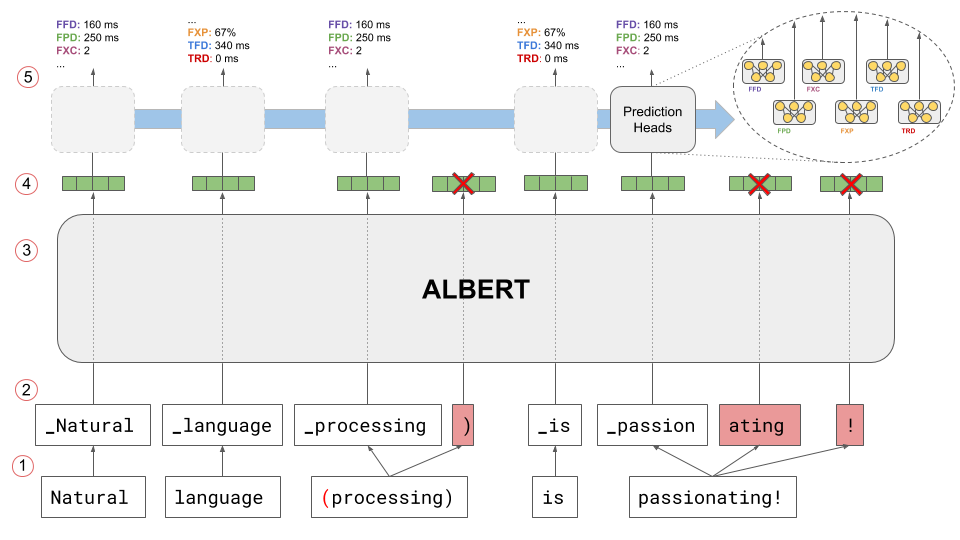
\includegraphics[width=1\linewidth]{figures/appendix/A3_multitask_et} 

}

\caption{Multi-task token-level regression on eye-tracking annotations. Preceding punctuation is removed (1), and the sentence is tokenized while keeping track of non-initial tokens (2). Embeddings are fed to the ALBERT model (3), and non-initial representations are masked to ensure a one-to-one mapping between labels and predictions (4). Finally, task-specific prediction heads are used to predict gaze metrics in a multitask setting with hard parameter sharing (5).}\label{fig:multitask-et}
\end{figure}

A multitask token-level regression fine-tuning approach was adopted throughout this study to predict eye-tracking metrics using neural language models. This novel approach's choice stems from the fact that the regression task of predicting gaze metrics is inherently word-based given the granularity of eye-tracking annotations and that different gaze metrics provide complementary viewpoints over multiple stages of cognitive processing and can as such be modeled more precisely in a multitask learning setting. Figure \ref{fig:multitask-et} presents the model's training and inference procedure, closely matching other approaches used to train neural language models for sequence tagging tasks like POS tagging and named entity recognition.

The most defining detail in the procedure is the need to preserve an exact one-to-one mapping between input words and gaze metrics annotations, which is non-trivial in light of subword tokenization approaches that represent nowadays the \emph{de facto} standard for training modern neural language models. To enforce such mapping, two steps are taken. First, all initial punctuation (e.g.~the open parenthesis before \emph{processing} in Figure \ref{fig:multitask-et} example) is removed to make the initial subword token for that word (i.e.~the one preceded by whitespace) equal to the word's first characters. Then, all non-initial subword tokens are identified in step (2), and their respective embeddings are masked in step (4) before passing the remaining initial embeddings (one per whitespace-tokenized word at this point, as for gaze metrics) to the set of prediction heads responsible for inferring individual gaze metrics. While this procedure can be regarded as suboptimal since not all learned representations are used for prediction, it is essential to remember that all the embeddings produced by attention-based neural language models are contextualized and encode information about the entire sentence and surrounding context to some extent. In this sense, initial token embeddings can be trained in this setting to predict gaze metrics relative to the whole word, effectively bypassing the issues about information loss raised by the masking procedure.

Another important detail in the training and inference procedure is the standardization of metrics, which plays a key role in this setup due to the different ranges of different metrics (e.g.~fixation probability is always defined in the interval \([0,1]\), while gaze durations are integers in the scale of hundreds/thousands of milliseconds). Specifically, considering the set \(X\) of values assumed by a specific metric for all tokens in the eye-tracking datasets, the average \(\mu_X\) and standard deviation \(\sigma_X\) of those values are computed, and each value is transformed as:
\begin{equation}
X_i' = \frac{X_i - \mu_X}{\sigma_X}
\end{equation}
to produce a new range \(X'\) with average equal to \(0\) and standard deviation equal to \(1\). Predicted values are then reconverted to the original scale as \(X_i = (X'_i \cdot \sigma_X) + \mu_X\) when performing inference, and training and testing metrics are computed on each metric's original scale.

\paragraph{Spillover concatenation} Cognitive processing literature reports evidence of reading times for a word being shaped not only by the predictability of the word itself but also by the predictability of the words that precede it \autocite{smith-levy-2013-effect} in what is commonly referred to as the \emph{spillover effect} \autocite{mitchell-1984-evaluation}. The existence of spillover has important implications in the context of this gaze metrics prediction approach since the embeddings for a single word may not contain enough information to predict the influence of preceding tokens in shaping reading behaviors. Notably, \textcite{schjindel-linzen-2020-single} include the surprisal of the three previous words in a mixed-effect model used to estimate a surprisal-to-reading-times conversion coefficient. While it can be hypothesized that in this approach, the usage of contextualized word embeddings can automatically account for this type of interaction, the effect of leveraging preceding tokens for the current token's metric prediction is assessed to confirm this hypothesis. A new procedure defined as \emph{spillover concatenation} is introduced for this purpose, in which token embeddings are augmented by performing a rolling concatenation of the \(n\) preceding embeddings before feeding the final representation to prediction heads. Initial tokens are padded with \(0\) vectors to match the fixed size defined by embedding size and the \(n\) parameter. For example, using spillover concatenation with \(n = 3\) within a BERT model with a hidden size of 768 involves having prediction heads taking input size of \(768 \cdot (3 + 1) = 3072\), the size of the token embedding for which gaze metrics should be predicted plus the size of the three preceding token embeddings. In this way, information about preceding tokens is explicitly included at prediction time.

Figure \ref{fig:spillover-training} shows the validation losses during training for the two models used in the experiments of Chapter \ref{chap:ex3} with their counterparts using spillover concatenation. Model performances are not positively influenced by introducing the concatenation technique and remain very similar for both architectures.



\begin{figure}

{\centering 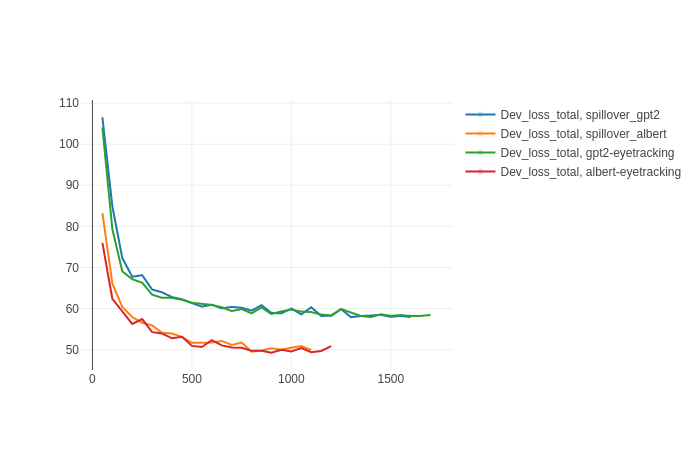
\includegraphics[width=0.7\linewidth]{figures/appendix/A3_spillover_training} 

}

\caption{Validation total loss for GPT-2 and ALBERT over a split of the eye-tracking merged corpora with and without spillover concatenation. Model predictive performances were comparable across training and testing for the two models.}\label{fig:spillover-training}
\end{figure}

\paragraph{Model performances} Table \ref{tab:multitask-et-scores} presents the test performances of ALBERT and GPT-2 models trained with and without the spillover concatenation approach on the merge of all eye-tracking corpora. The top two rows present descriptive statistics about extreme values, the mean and standard deviation in annotations averaged across participants for each metric. It is interesting to observe that the maximum value observed for first pass duration (FPD) is higher than the one for total fixation duration (TFD). While this situation would not be possible in practice due to first pass duration being included in total reading times, it reminds us about the approximate nature of our filling-and-averaging procedure described in Appendix \ref{app:et-metrics}. Comparing results to those of Table \ref{tab:ex1-results}, where gaze metrics were modeled at the sentence level, we observe much worse results in terms of explained variance for both models: while fixations and first pass duration (FXC, FXP, FPD) are generally well modeled, worse results are obtained for first and total fixation durations (FFD, TFD), and in particular for the duration of regression (TRD). These results can be attributed to the merging of different corpora that, being annotated by different participants, present very different properties, as shown in Table \ref{tab:et-corpora} and Figure \ref{fig:surprisal-ratios}. While on the one hand, this choice harms modeling performances, on the other hand, it provides us with more representative results for the general setting.

\begin{table}[!h]

\caption{\label{tab:multitask-et-scores}Descriptive statistics and model performances for the merged eye-tracking training corpus. Model scores are in format $\text{RMSE}_{\text{MAX}}|R^2$, where RMSE is the root-mean-squared error and MAX is the max error for model predictions.}
\centering
\fontsize{11}{13}\selectfont
\begin{tabular}[t]{lcccccc}
\toprule
\textbf{} & \textbf{FFD} & \textbf{FPD} & \textbf{FXP} & \textbf{FXC} & \textbf{TFD} & \textbf{TRD}\\
\midrule
min-max value & $0-986$ & $0-2327$ & $0-1$ & $0-8.18$ & $0-1804$ & $0-4055$\\
$\mu|\sigma$ statistics & $162|50$ & $188|86$ & $.56|.27$ & $.85|.53$ & $206|87$ & $90|122$\\
\hline
ALBERT & $41_{78}|.33$ & $61_{121}|.50$ & $.17_{.32}|.60$ & $.31_{.62}|.66$ & $65_{132}|.44$ & $110_{207}|.19$\\
ALBERT Spillover & $41_{78}|.33$ & $61_{122}|.50$ & $.17_{.33}|.60$ & $.31_{.62}|.66$ & $65_{132}|.44$ & $110_{208}|.19$\\
\hline
GPT-2 & $44_{83}|.23$ & $68_{136}|.37$ & $.18_{.35}|.56$ & $.36_{.70}|.54$ & $74_{149}|.28$ & $115_{222}|.11$\\
GPT-2 Spillover & $43_{83}|.26$ & $68_{135}|.37$ & $.19_{.35}|.50$ & $.36_{.70}|.54$ & $73_{146}|.30$ & $116_{220}|.10$\\
\bottomrule
\end{tabular}
\end{table}

In general, better performances are observed for the masked language model ALBERT, suggesting the importance of having access to bidirectional context for gaze metrics prediction. Results present additional evidence supporting the superfluity of the spillover concatenation procedure, which was henceforth dropped in the context of Chapters \ref{chap:ex2} and \ref{chap:ex3}'s experiments. Although good scores in terms of average and maximal errors are observed for all metrics, the relatively low \(R^2\) seem to suggest that large margins of improvement are still available in the context of gaze metrics predictions with neural language models.

\hypertarget{app:intra-sim}{%
\chapter{Intra-model Similarity for All Models}\label{app:intra-sim}}

\vspace{-5em}





\begin{figure}[H]

{\centering \subfloat[RSA score, CLS token\label{fig:intra-pc-1}]{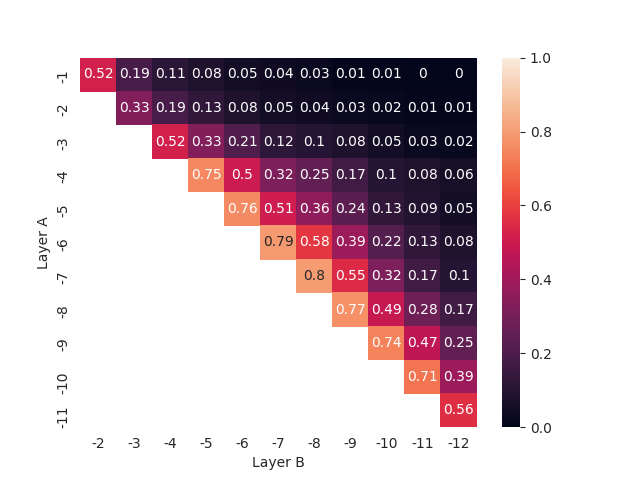
\includegraphics[width=0.48\linewidth]{figures/appendix/A4_rsa_intra_cls_pc} }\subfloat[PWCCA distance, CLS token\label{fig:intra-pc-2}]{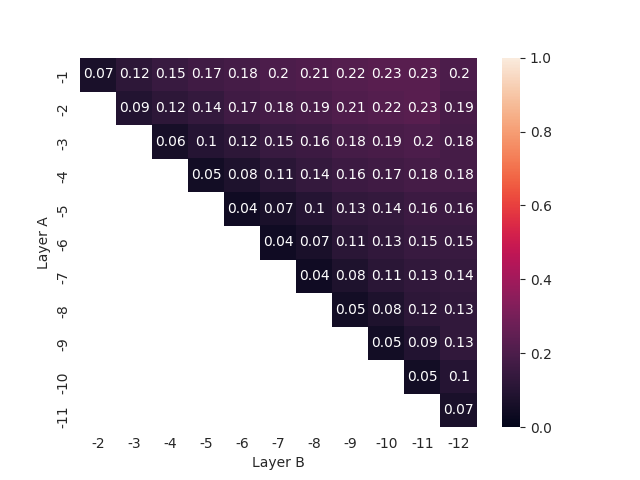
\includegraphics[width=0.48\linewidth]{figures/appendix/A4_pwcca_intra_cls_pc} }\newline\subfloat[RSA score, tokens' average\label{fig:intra-pc-3}]{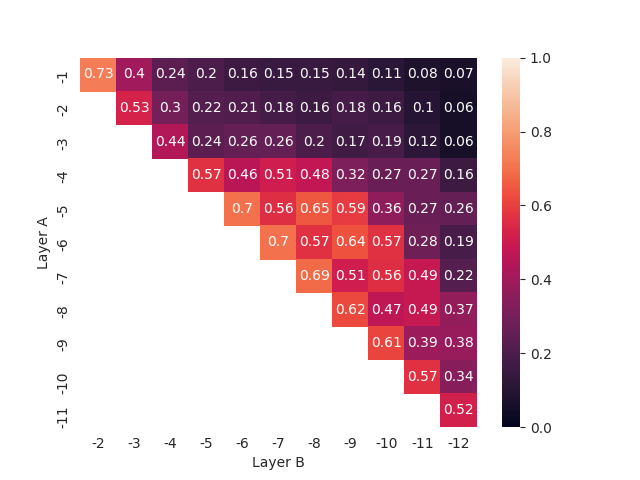
\includegraphics[width=0.48\linewidth]{figures/appendix/A4_rsa_intra_mean_pc} }\subfloat[PWCCA distance, tokens' average\label{fig:intra-pc-4}]{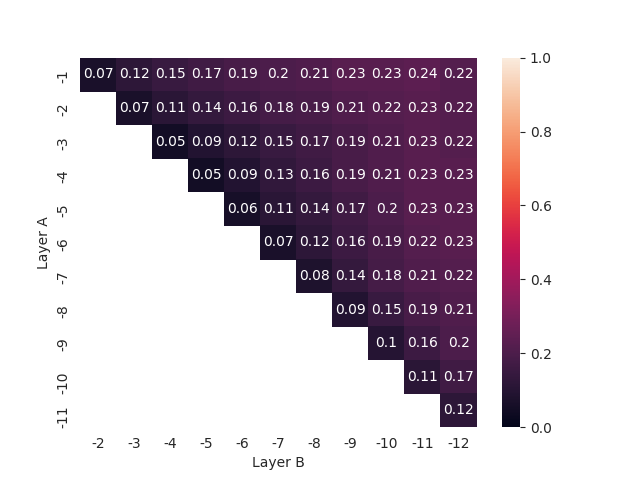
\includegraphics[width=0.48\linewidth]{figures/appendix/A4_pwcca_intra_mean_pc} }\newline\subfloat[RSA score, all tokens\label{fig:intra-pc-5}]{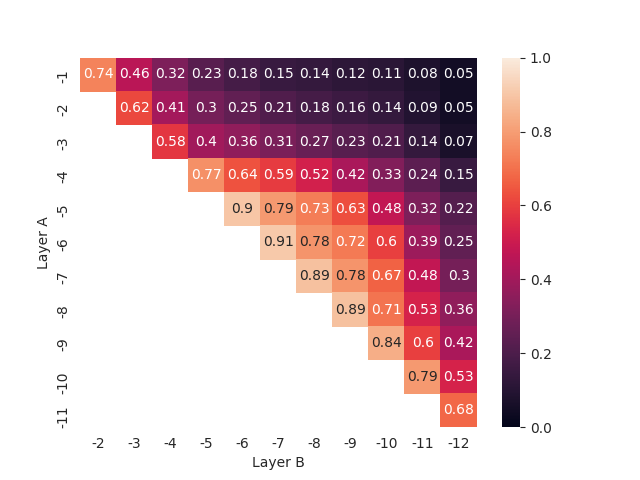
\includegraphics[width=0.48\linewidth]{figures/appendix/A4_rsa_intra_tokens_pc} }\subfloat[PWCCA distance, all tokens\label{fig:intra-pc-6}]{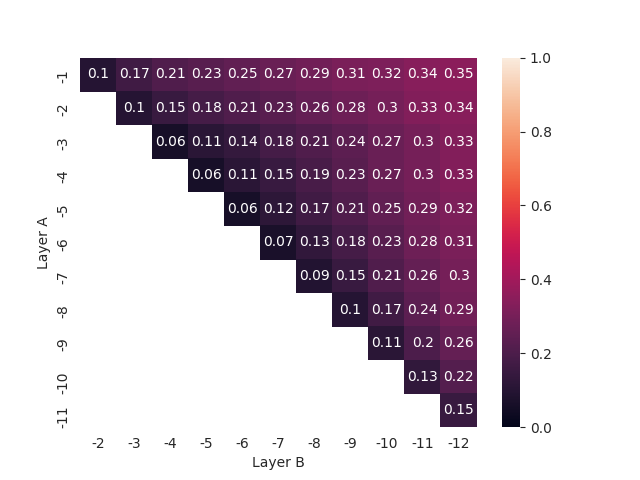
\includegraphics[width=0.48\linewidth]{figures/appendix/A4_pwcca_intra_tokens_pc} }

}

\caption{Intra-model RSA and PWCCA scores across layers' combinations for the ALBERT model fine-tuned on perceived complexity (\textbf{PC}). Layer -1 is the last layer before prediction heads.}\label{fig:intra-pc}
\end{figure}





\begin{figure}

{\centering \subfloat[RSA score, CLS token\label{fig:intra-et-1}]{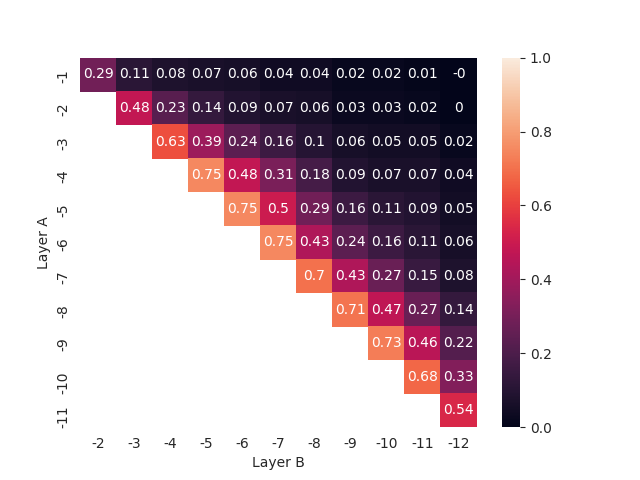
\includegraphics[width=0.5\linewidth]{figures/appendix/A4_rsa_intra_cls_et} }\subfloat[PWCCA distance, CLS token\label{fig:intra-et-2}]{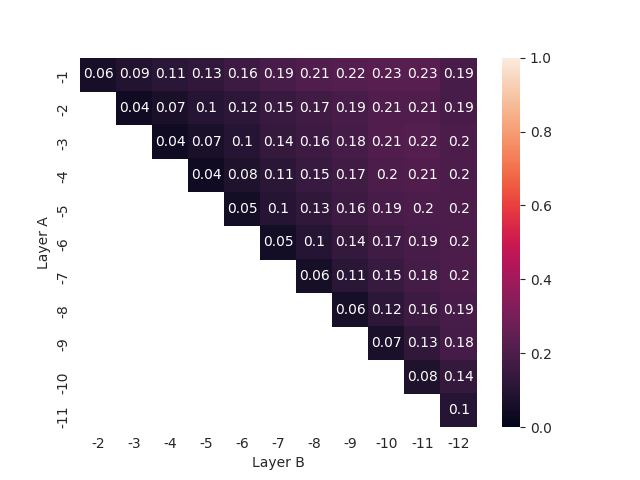
\includegraphics[width=0.5\linewidth]{figures/appendix/A4_pwcca_intra_cls_et} }\newline\subfloat[RSA score, tokens' average\label{fig:intra-et-3}]{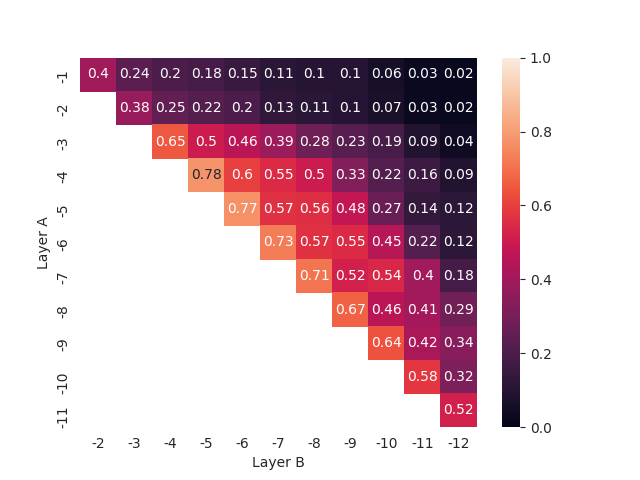
\includegraphics[width=0.5\linewidth]{figures/appendix/A4_rsa_intra_mean_et} }\subfloat[PWCCA distance, tokens' average\label{fig:intra-et-4}]{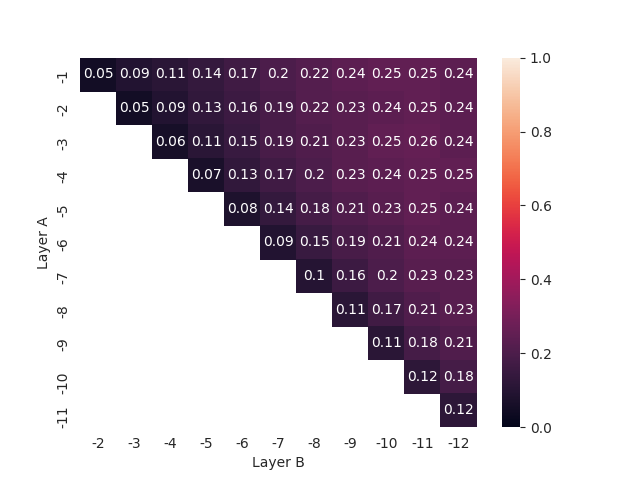
\includegraphics[width=0.5\linewidth]{figures/appendix/A4_pwcca_intra_mean_et} }\newline\subfloat[RSA score, all tokens\label{fig:intra-et-5}]{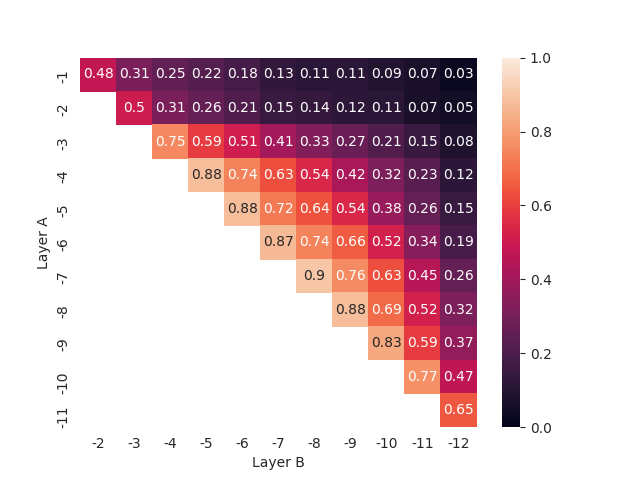
\includegraphics[width=0.5\linewidth]{figures/appendix/A4_rsa_intra_tokens_et} }\subfloat[PWCCA distance, all tokens\label{fig:intra-et-6}]{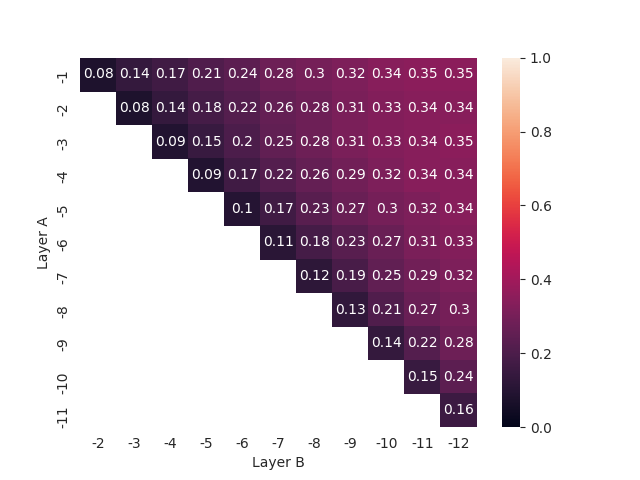
\includegraphics[width=0.5\linewidth]{figures/appendix/A4_pwcca_intra_tokens_et} }

}

\caption{Intra-model RSA and PWCCA scores across layers' combinations for the ALBERT model fine-tuned in parallel on gaze metrics (\textbf{ET}). Layer -1 corresponds to the last layer before prediction heads.}\label{fig:intra-et}
\end{figure}





\begin{figure}

{\centering \subfloat[RSA score, CLS token\label{fig:intra-ra-1}]{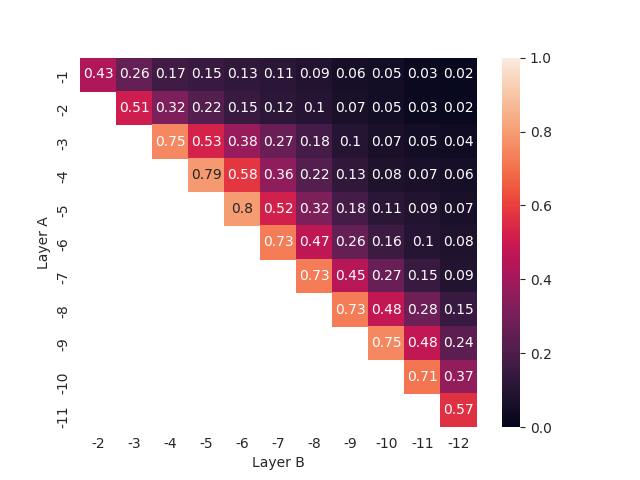
\includegraphics[width=0.5\linewidth]{figures/appendix/A4_rsa_intra_cls_ra} }\subfloat[PWCCA distance, CLS token\label{fig:intra-ra-2}]{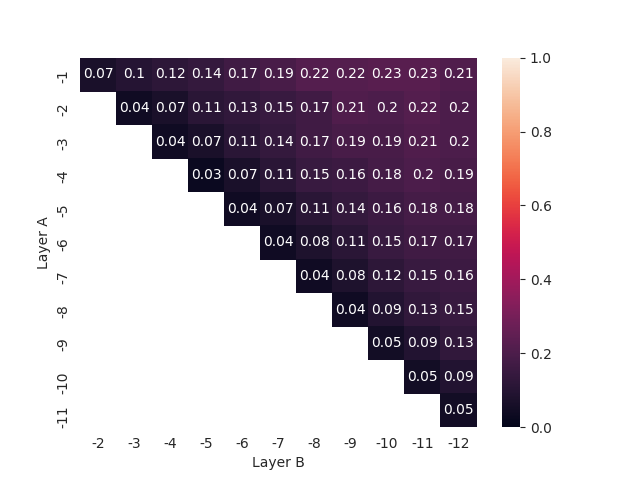
\includegraphics[width=0.5\linewidth]{figures/appendix/A4_pwcca_intra_cls_ra} }\newline\subfloat[RSA score, tokens' average\label{fig:intra-ra-3}]{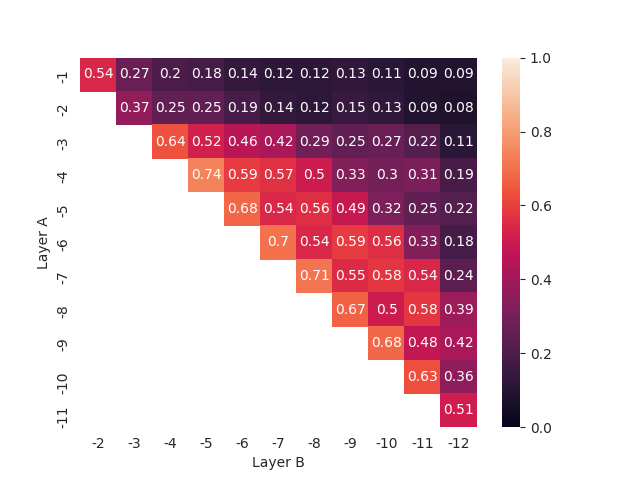
\includegraphics[width=0.5\linewidth]{figures/appendix/A4_rsa_intra_mean_ra} }\subfloat[PWCCA distance, tokens' average\label{fig:intra-ra-4}]{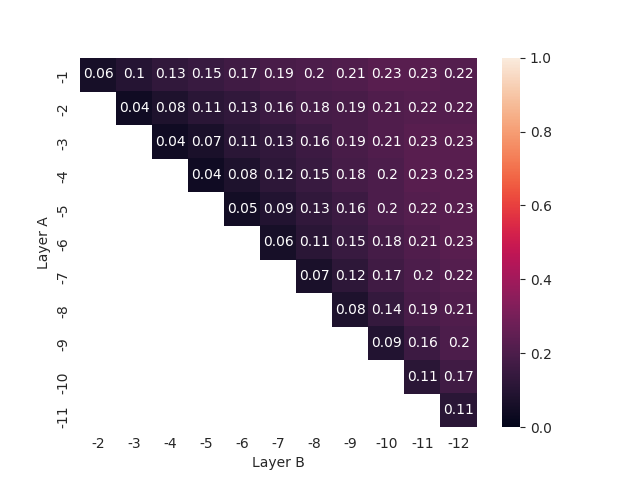
\includegraphics[width=0.5\linewidth]{figures/appendix/A4_pwcca_intra_mean_ra} }\newline\subfloat[RSA score, all tokens\label{fig:intra-ra-5}]{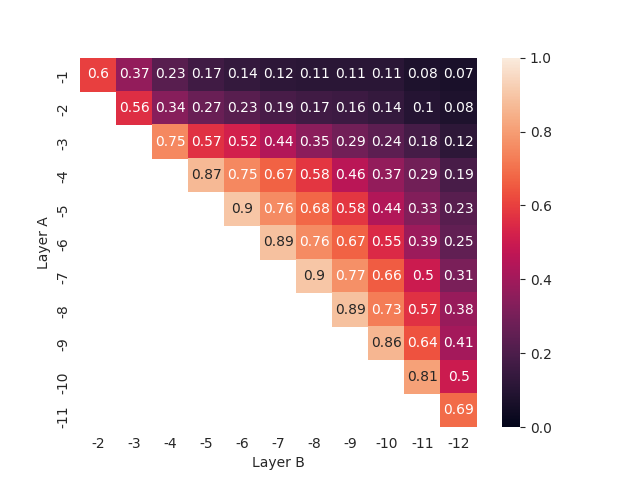
\includegraphics[width=0.5\linewidth]{figures/appendix/A4_rsa_intra_tokens_ra} }\subfloat[PWCCA distance, all tokens\label{fig:intra-ra-6}]{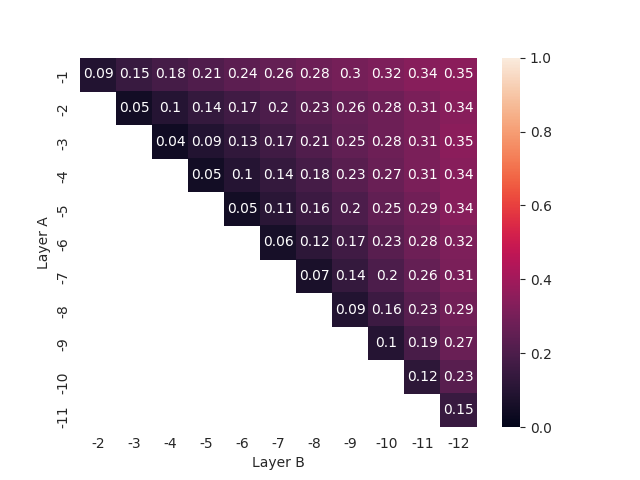
\includegraphics[width=0.5\linewidth]{figures/appendix/A4_pwcca_intra_tokens_ra} }

}

\caption{Intra-model RSA and PWCCA scores across layers' combinations for the ALBERT model fine-tuned on readability assessment annotations (\textbf{RA}). Layer -1 corresponds to the last layer before prediction heads.}\label{fig:intra-ra}
\end{figure}

\hypertarget{app:garden-paths-et}{%
\chapter{Gaze Metrics Predictions for Garden Path Sentences}\label{app:garden-paths-et}}



\begin{figure}[H]

{\centering 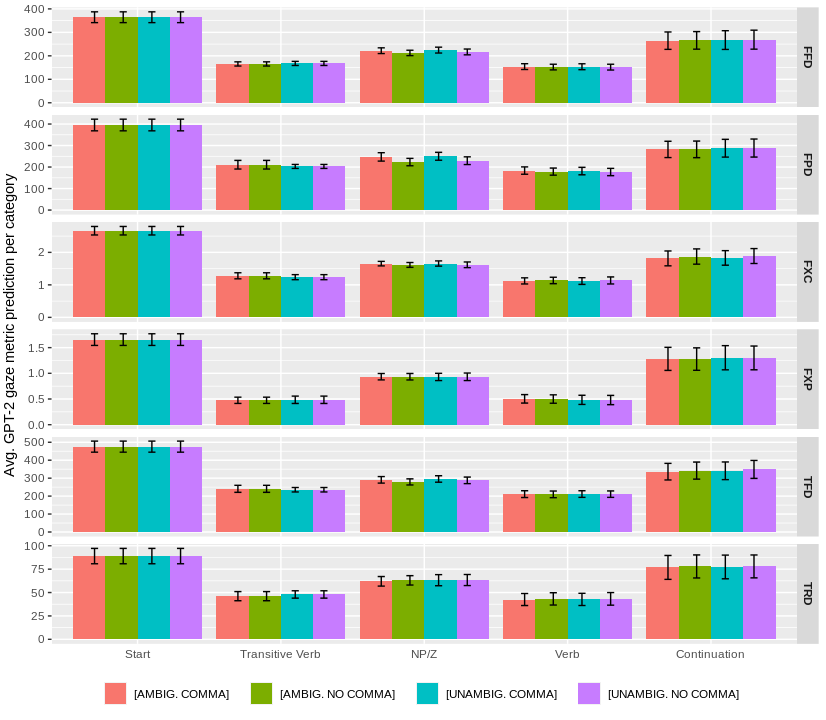
\includegraphics[width=1\linewidth]{figures/appendix/A5_gpt2_npz_ambig_et} 

}

\caption{Average GPT2-ET gaze metrics predictions for the ``NP/Z Ambiguity with Verb Transitivity'' SyntaxGym test suite. Bars show 95\% confidence intervals. Units are in ms for durations, \% for FXP, and raw counts for FXC.}\label{fig:gpt2-npz-ambig-et}
\end{figure}



\begin{figure}

{\centering 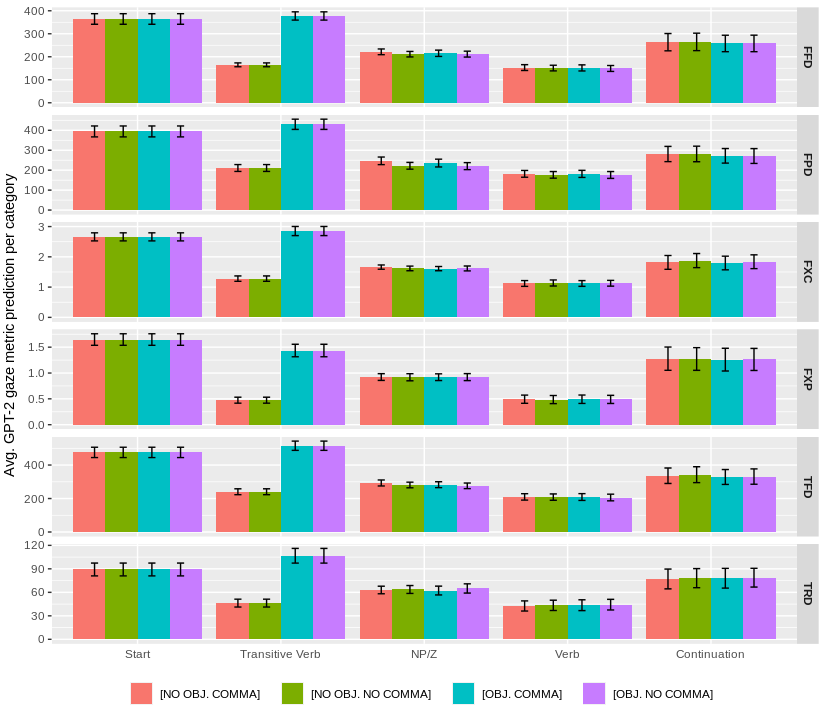
\includegraphics[width=1\linewidth]{figures/appendix/A5_gpt2_npz_obj_et} 

}

\caption{Average GPT2-ET gaze metrics predictions for the ``NP/Z Ambiguity with Overt Object'' SyntaxGym test suite. Bars show 95\% confidence intervals. Units are in ms for durations, \% for FXP, and raw counts for FXC.}\label{fig:gpt2-npz-obj-et}
\end{figure}



\begin{figure}

{\centering 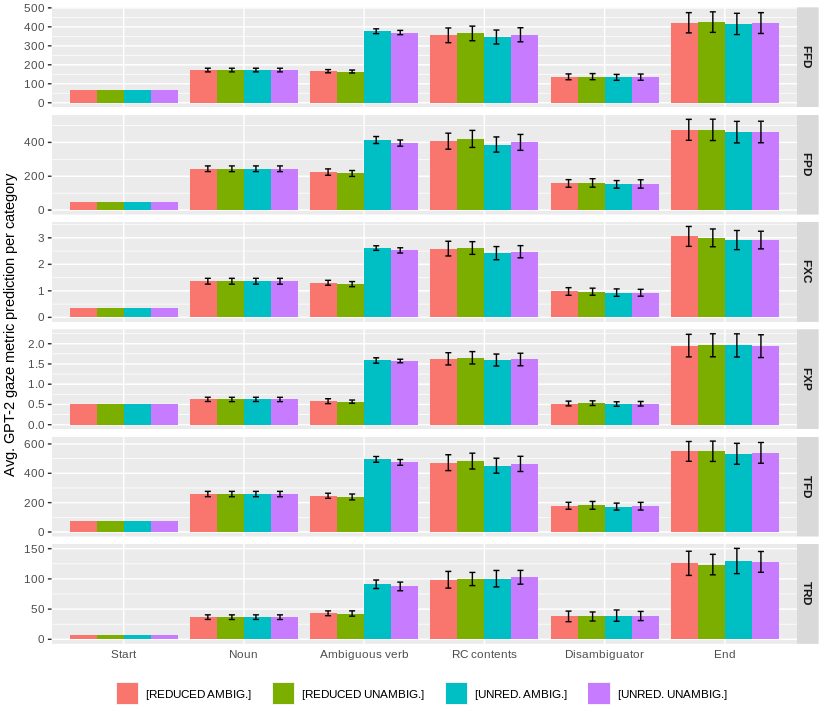
\includegraphics[width=1\linewidth]{figures/appendix/A5_gpt2_mvrr_et} 

}

\caption{Average GPT2-ET gaze metrics predictions for the ``MV/RR Ambiguity'' SyntaxGym test suite. Bars show 95\% confidence intervals. Units are in ms for durations, \% for FXP, and raw counts for FXC.}\label{fig:gpt2-mvrr-et}
\end{figure}

\hypertarget{app:params}{%
\chapter{Reproducibility and Environmental Impact}\label{app:params}}

\begin{table}[!h]

\caption{\label{tab:train-params}Variable training parameters used in the experiments of this study. MTL stands for multitask learning.}
\centering
\fontsize{11}{13}\selectfont
\begin{tabular}[t]{lcc>{}c|cc>{}c|cc}
\toprule
\multicolumn{1}{c}{\textbf{ }} & \multicolumn{3}{c}{\textbf{Chapter 3}} & \multicolumn{3}{c}{\textbf{Chapter 4}} & \multicolumn{2}{c}{\textbf{Chapter 5}} \\
\cmidrule(l{3pt}r{3pt}){2-4} \cmidrule(l{3pt}r{3pt}){5-7} \cmidrule(l{3pt}r{3pt}){8-9}
 & PC & ET & Probes & PC & ET & RA & ALBERT & GPT-2\\
\midrule
fine-tuning & standard & MTL & MTL & standard & MTL & standard & MTL & MTL\\
granularity & sent. & sent. & sent. & sent. & word & sent. & word & word\\
freeze LM $w$ & ❌ & ❌ & ✅ & ❌ & ❌ & ❌ & ❌ & ❌\\
weighted loss & - & ✅ & ❌ & - & ❌ & - & ❌ & ❌\\
CV folds & 5 & 5 & 5 & - & - & - & - & -\\
early stopping & ✅ & ✅ & ❌ & ✅ & ✅ & ✅ & ✅ & ✅\\
training epochs & 15 & 15 & 5 & 15 & 15 & 15 & 15 & 15\\
patience & 5 & 5 & - & 5 & 5 & 5 & 5 & 5\\
evaluation steps & 20 & 40 & - & 20 & 100 & 80 & 100 & 100\\
\bottomrule
\end{tabular}
\end{table}

\paragraph{Tools} Experiments were executed on a Ubuntu 18.04 LTS server, using a NVIDIA K40 GPU with 12GB RAM and CUDA 10.1. Relevant Python libraries used throughout the study with their respective versions are: 🤗 \texttt{transformers\ 2.11.0} for accessing pre-trained Transformer language models, \texttt{farm\ 0.4.5} for multitask learning, \texttt{torch\ 1.3.0} as a backed for deep learning, and \texttt{syntaxgym\ 0.5.3} for Chapter \ref{chap:ex3} experiments. Python 3.6.3 was used for all training scripts. A custom adaptation of the Oxforddown template was used for this thesis.\footnote{\url{https://github.com/AI-Student-Society/thesisdown-it}} Code for reproducibility purposes is available at the address \url{https://github.com/gsarti/interpreting-complexity}.

\paragraph{Model Training} Table \ref{tab:train-params} present the set of variable training parameters used in all the experiments of this study. Besides those, a set of fixed parameters was also used: all experiments were performed using a batch size of 32 observations, a maximum sequence length of 128 tokens, a linear training schedule with one-tenth of total steps used as warmup steps, the \emph{AdamW} optimizer \autocite{loshchilov-hutter-2019-decoupled} with weight decay equal to \(0.01\), and a learning rate of \(10^{-5}\). No hyperparameter search was performed due to time limitations.

\paragraph{Tokenization} All tokenizers used in the experiments used cased text and were based respectively on the SentencePiece approach \autocite{kudo-richardson-2018-sentencepiece} for ALBERT and a custom version of Byte-Pair Encoding tokenization \autocite{sennrich-etal-2016-neural} with token-like whitespaces for GPT-2. Default \texttt{AlbertTokenizer} and \texttt{GPT2Tokenizer} classes available in the 🤗 \texttt{transformers} library with pretrained tokenizers were used for this purpose. The vocabulary used by those had size 30'000 for ALBERT and 50'257 for GPT-2, including special tokens.

\paragraph{Architecture} The default parameters for the 🤗 \texttt{transformers} checkpoints of ALBERT and GPT-2 (specifically, \texttt{albert-base-v2} and \texttt{gpt2} in the Model Hub) were used for this study. Concretely, this means embeddings and hidden sizes of 128 and 3072 for ALBERT and tied embedding-hidden size of 768 for GPT-2, 12 transformer blocks using 12 heads for multi-head self-attention each, and a smoothed variant of the Gaussian Error Linear Unit (GELU) as nonlinearity \autocite{hendrycks-gimpel-2016-gaussian}. GPT-2 has an embedding and attention dropout rate of 0.1 and a layer normalization \autocite{ba-etal-2016-layer} epsilon of \(10^{-5}\), while ALBERT employs a classifier dropout rate of 0.1 and a layer normalization epsilon of \(10^{-12}\).

\paragraph{CO2 Emissions Related to Experiments} Experiments were conducted using the private infrastructure of the ItaliaNLP Lab\footnote{\url{https://www.italianlp.it}} at the Institute for Computational Linguistics ``A. Zampolli'' (ILC-CNR) in Pisa, which has an estimated carbon efficiency of 0.321 kgCO\(_2\)eq/kWh \autocite{moro2018electricity}. A cumulative of roughly 100 hours of computation was performed on a Tesla K40 GPU (TDP of 245W). Total emissions are estimated to be 7.86 kgCO\(_2\)eq. Estimations were conducted using the Machine Learning Impact Calculator\footnote{\url{https://mlco2.github.io/impact\#compute}} presented in \textcite{lacoste2019quantifying}.

In-detail reports of all experimental runsre produced automatically using the MLFlow\footnote{\url{https://mlflow.org/}} tool and are available at the following address: \url{https://public-mlflow.deepset.ai/\#/experiments/99}.


%%%%% REFERENCES

% JEM: Quote for the top of references (just like a chapter quote if you're using them).  Comment to skip.
% \begin{savequote}[8cm]
% The first kind of intellectual and artistic personality belongs to the hedgehogs, the second to the foxes \dots
%   \qauthor{--- Sir Isaiah Berlin \cite{berlin_hedgehog_2013}}
% \end{savequote}

\setlength{\baselineskip}{0pt} % JEM: Single-space References

{\renewcommand*\MakeUppercase[1]{#1}%
\printbibliography[heading=bibintoc,title={\bibtitle}]}

\end{document}
